\chapterillustration{abertura-afim}{abertura-afim-professor}

\chapterwhat{Funções linear e afim e suas representações algébrica e gráfica, taxa de variação, proporcionalidade direta, funções afins de domínio discreto (Progressões Aritméticas), Aplicações.}

\chapterbecause{O modelo de variação constante é um dos modelos mais presentes em observações científicas e até mesmo em nosso cotidiano. Ele pode ser identificado por exemplo, em relações que modelam a compra/consumo e venda, o esvaziamento de um recipiente por um ralo em função do tempo ou na relação entre distância e tempo do “movimento uniforme” estudado pela Cinemática, entre tantos outros. Um caso particularmente importante é aquele em que há proporcionalidade entre as grandezas envolvidas na modelagem. As ide ias desenvolvidas neste capítulo servem como base para aplicações em diversas áreas.}

\chapter{Função Afim}

%%%% Página de créditos

\autorum{Gladson Antunes (UNIRIO)}
\autordois{Michel Cambrainha (UNIRIO)}
\autortres{Bruno Vianna (Colégio Pedro II)}

\revisorum{Cydara Ripoll}
\revisordois{Letícia Rangel}

\versao{1.2}

\graficos{Beatriz Cabral e Tarso Caldas}
\ilustracao{Miller  Guglielmo}

\autordacapa{Scott Webb}{Unsplash}{https://unsplash.com/photos/fMUIVein7Ng}

%Licença cc-by-sa
\ccbysa

% Link para versão digital:
\versaodigital{https://www.umlivroaberto.org/BookCloud/Volume_1/master/view/AF107.html}

\creditos


\mainmatter

\begin{apresentacao}{Introdução}

\subsection{Habilidades e pré-requsitos}

Neste capítulo contemplam-se as seguintes habilidades da segunda versão da \href{http://historiadabncc.mec.gov.br/documentos/bncc-2versao.revista.pdf}{Base Nacional Comum Curricular (BNCC):}

\begin{habilities}{EM11MT07}

Reconhecer função afim e suas representações algébrica e gráfica, identificar o modelo de variação e a taxa de variação, incluindo os casos em que a variação é proporcional (linear), e utilizar essas noções para representar e resolver problemas como os de Movimento Uniforme, entre outros.
\end{habilities}

Os pré-requisitos para este capítulo são:

\begin{habilities}{EF07MA13} Resolver e elaborar problemas que envolvam variação de proporcionalidade direta e de proporcionalidade inversa entre duas grandezas, utilizando sentença algébrica para expressar a relação entre elas.

\tcbsubtitle{EF07MA14} Resolver e elaborar problemas que possam ser representados por equações polinomiais de 1º grau, redutíveis à forma \(ax+b=c\), fazendo uso das propriedades da igualdade.
\end{habilities}

Além disso há outras habilidades que se relacionam com os conceitos abordados nesse capítulo, a saber,

\begin{habilities}{EF09MA05} Resolver e elaborar problemas que envolvam porcentagens, com a ideia de aplicação de percentuais sucessivos e a determinação das taxas percentuais, preferencialmente com o uso de tecnologias digitais, no contexto da educação financeira.

\tcbsubtitle{EF09MA07} Resolver problemas que envolvam a razão entre duas grandezas de espécies diferentes, como velocidade e densidade demográfica.

\tcbsubtitle{EF09MA08} Resolver e elaborar problemas que envolvam relações de proporcionalidade direta e inversa entre duas ou mais grandezas, inclusive escalas, divisão em partes proporcionais e taxa de variação, em contextos socioculturais, ambientais e de outras áreas.

\end{habilities}

Prezado colega, o presente capítulo foi concebido a partir de uma abordagem de função afim não usual. Deixamos a cargo do aluno levantar conjecturas a respeito dos conceitos, definições e propriedades da função afim. Essas conjecturas ou indagações são provocadas por meio de atividades que abordam os conceitos a serem trabalhados.
\columnbreak

Iniciamos o capítulo resgatando a ideia de grandezas proporcionais e relacionando-a com o conceito de função linear. É comum que a noção de proporcionalidade, mais especificamente a de proporcionalidade direta, amplamente vinculada à “regra de três”, seja associada pelos estudantes a qualquer variação entre grandezas. Ainda que, de fato, a proporcionalidade tenha um papel de destaque em modelos da física e da química, nem toda variação entre grandezas é um modelo desse tipo. Portanto acreditamos que, na condução das atividades seja natural para o professor (e recomendamos que o faça) chamar a atenção dos estudantes para o fato que existem grandezas cuja relação não é de proporcionalidade.

Busque com seus estudantes desenvolver as atividades, de maneira a deixá-los livres para criar conjecturas ou até mesmo a chegar a conclusões, por meio de argumentos diversos, sejam eles visuais, geométricos, algébricos, lógicos ou até mesmo dissertativos.

Vale ressaltar alguns pontos:
\begin{itemize}
\item {} 
Boa parte das atividades tem como objetivo apontar para os estudantes a importância da análise da taxa de variação para inferirmos se uma função é afim ou não. Neste capítulo, resolvemos não fazer uso do termo \textbf{coeficiente angular} da reta. Essa decisão se pauta em dois aspectos: (i) Dependendo da escolha da unidade para as grandezas envolvidas, a imagem da representação gráfica pode sugerir um ângulo cuja a tangente não correspnde ao coeficiente angular da reta determinada pela função, e assim levar ao equívoco. (ii) Além disso, acreditamos que a compreensão de taxa de variação pode ser mais fácil se dotada de significado. Assim, por exemplo, é mais fácil compreender a taxa de variação entre temperatura e altitude ou entre velocidade e tempo do que associar essa ideia a um conceito essencialmente numérico, que é o caso do coeficiente angular de uma reta. O ângulo tem apelo visual independente das escalas escolhidas para os eixos, e assim, chamar a taxa de variação de coeficiente angular pode trazer confusão. Portanto, neste texto, optamos por destacar a especificidade de cada conceito associando o termo taxa de variação à função afim e coeficiente angular a retas (desde que estejam em um sistema de coordenadas cujos eixos apresentam-se na mesma escala).

\item {} 
Também não achamos adequado o termo \emph{coeficiente linear} para o \(b\) em \(f(x)=ax+b\). Primeiramente porque, quando ele é não nulo a função deixa de ser “linear”, então ele funciona mais como uma medida da “não-linearidade” da função. Em alguns livros ele também é chamado de \emph{intercepto}. Também optamos por não utilizar essa nomenclatura por ela ser restringir apenas aos casos em que os eixos estão na posição tradicional (isto é, se cruzando no \((0,0)\)) e além disso, \(0\) deve pertencer ao domínio da função em questão. Por essas razões, resolvemos não dar um nome para o “\(b\)”, apenas lhe dar um significado geométrico que serve em qualquer situação: a medida da translação vertical que se faz no gráfico da função linear \(\ell(x)=ax\) para se obter o gráfico da função \(f(x)=ax+b\).

\item {} 
Em alguns livros o capítulo tem o nome de “Função do 1° grau”. Também acreditamos que esse termo é equivocado pois função não tem grau, o que tem grau é polinômio. No entanto, podemos dizer que toda função afim pode ser expressa por um polinômio do 1° grau.

\clearpage
\item {} 
Também é comum, apresentarmos uma função afim da forma \(f(x)=ax+b\), sem nos preocuparmos se o seu domínio é toda real ou não. Algumas atividades abordam funções com domínios discretos, outras cujos domínios são intervalos reais. Sendo assim, ressalte para seus estudantes a importância do domínio da função, como por exemplo: \(f:\mathbb{R}\to\mathbb{R}\) onde \(f(x)=2x+1\) ; \(g:[0,2]\to \mathbb{R}\) onde \(g(x) = -2x\)   e  \(h:\mathbb{N}\to\mathbb{R}\) onde \(h(n)=3n-5\); de maneira que o gráfico de \(f\) é uma reta; de \(g\) é um segmento de reta e de \(h\) é um conjunto de pontos colineares.

\item {} 
Pode ocorrer que algum estudante tente associar uma reta de inclinação negativa a uma relação de proporcionalidade inversa. Caso essa questão seja levantada durante a execução das atividades, mostre a seus estudantes, com um exemplo simples, como é a curva que representa a variação de proporcionalidade inversa (hipérbole). Decidimos não discutir esse assunto nesse capítulo para que não ficasse demasiadamente extenso.

\item {} 
Sempre que possível, utilize recursos computacionais para desenvolver o discutir as atividades propostas ou para gerar novas atividades. Isso torna o estudo mais dinâmico.  São propostas duas atividades que apresentam versões digitais criadas no Geogebra. Caso não consiga trabalhá-las em sala de aula, estimule seus estudantes a acessarem os respectivos links.

\item {} 
As habilidades que estão listadas como pré-requisitos são retomadas pelas atividades e eventualmente aprofundadas em relação à maneira como elas são tradicionalmente exploradas no Ensino Fundamental.

\end{itemize}

\textbf{Alguns distratores} (apontados pela literatura de pesquisa)
\begin{itemize}
\item {} 
A repetida confirmação da validade da proporcionalidade - juntamente com o status intuitivo que o conceito recebe gradualmente - pode conduzir a uma ideia errada: se houver uma relação entre duas variáveis, essa relação provavelmente é proporcional. Estudos mostram que existe uma tendência generalizada entre os estudantes americanos com idade de \(12\) a \(16\) anos de que, se uma figura aumentar de \(k\) vezes, a área e o volume dessa figura serão ampliados também de \(k\) vezes. \citep{Dooren-et-al-2005}

\item {} 
A pesquisa tem documentado dificuldades dos estudantes com o conceito de inclinação. Há confusões associadas ao cálculo da inclinação e à interpretação de funções lineares e seus gráficos. Os estudantes também apresentam dificuldades em relacionar gráficos a equações lineares e à noção de taxa de variação. Eles têm dificuldade em perceber a inclinação como uma razão e conectar tal razão ao modelo físico. \citep{Stump-1999}

\item {} 
Nem toda razão pode ser expressa por números racionais, o que vincula, por meio da proporcionalidade, a apresentação dos números irracionais. Isso sinaliza que nem todas as situações podem ser resolvidas recorrendo-se apenas aos números racionais. \citep{Silva-et-al-2013}

\end{itemize}
\end{apresentacao}

\def\currentcolor{session1}
\clearmargin
\begin{objectives}{Na piscina}
{
\begin{itemize}
\item Reconhecer uma relação de proporcionalidade entre grandezas a partir da análise gráfica e da construção e análise dos dados em uma tabela;

\item Conjecturar sobre a representação gráfica de grandezas diretamente proporcionais, associando-a a um conjunto de pontos colineares
\end{itemize}
}{1}{2}
\end{objectives}
\begin{sugestions}{Na piscina}
{
\begin{itemize}
\item Como primeira atividade do capítulo, priorize as ideias em detrimento do rigor matemático. Ajude seus estudantes a transcreverem suas ideias de maneira precisa, ainda que informais.
No item (b), podem surgir respostas como: a primeira coluna aumenta de “uma em uma hora” enquanto a segunda aumenta de “200 em 200 litros”; a segunda coluna é obtida multiplicando a primeira por 200; tabela gerada pela função f(n)=200⋅n com domínio {0,1,2,3,4,5}. Apesar de não serem consequências diretas da definição, estão corretas e serão tratadas ao longo do capítulo.
\end{itemize}
}{1}{2}
\end{sugestions}
\clearmargin
\begin{answer}{Na piscina}
{
\begin{enumerate}
\item Piscina 1

\adjustbox{valign=t}
{
\begin{tabular}{|c|c|}
\hline
\tcolor{Tempo ($h$)} & \tcolor{Volume (litros)} \\
\hline
0 & 0 \\
\hline
1 & 200 \\
\hline
2 & 400 \\
\hline
3 & 600 \\
\hline
4 & 800 \\
\hline
5 & 1000 \\
\hline
\end{tabular}
}

\vspace{2em}

Piscina 2

\adjustbox{valign=t}
{
\begin{tabular}{|c|c|}
\hline
\tcolor{Tempo ($h$)} & \tcolor{Volume (litros)} \\
\hline
0 & 0 \\
\hline
1 & 150 \\
\hline
2 & 200 \\
\hline
3 & 300 \\
\hline
4 & 500 \\
\hline
5 & 800 \\
\hline
6 & 900 \\
\hline 
7 & 950 \\
\hline
8 & 1000 \\
\hline
\end{tabular}
}

\vspace{2em}


\item Sim, pois para $k\in\{0,2,3,4,5\}$ tempo
\[\begin{array}{ccc}
x\quad &\overline{\quad \quad \quad}& \quad y \\
k\cdot 1 \quad &\overline{\quad \quad \quad}& \quad k\cdot 200
\end{array}\]

\item Não, pois ao final da primeira hora o volume total de água aumentou 150 litros e na hora seguinte aumentou apenas 50 litros. Para haver proporcionalidade direta, deveria ter aumentado também 150 litros na segunda hora, totalizando 300 litros.
\end{enumerate}
}{1}
\end{answer}
\begin{sugestions}{Para refletir}
{
  Este é um convite à uma primeira reflexão sobre as propriedades geométricas de pontos colineares e sua relação com grandezas proporcionais. Conduza os seus estudantes a fazerem conjecturas sobre como deve ser a representação gráfica de grandezas diretamente proporcionais.
}{1}{1}
\end{sugestions}
\explore{Função Linear}\label{funcaolinear}
No capítulo de Funções, você foi apresentado ao conceito de função, uma relação entre duas grandezas que atende determinadas condições. Neste capítulo, pretendemos colocá-lo em contato com um dos modelos mais presentes em observações científicas e até mesmo em nosso cotidiano, o modelo de variação constante, aqui representado pelo conceito de função afim. Este modelo pode ser identificado por exemplo, em relações que modelam a compra/consumo e venda, o esvaziamento de um recipiente por um ralo em função do tempo ou na relação entre distância e tempo do “movimento uniforme” estudado pela Cinemática, entre tantos outros. Antes de estudarmos a função afim propriamente dita, vamos entender um de seus casos particulares, a função linear.

Comecemos analisando os seguintes problemas:

\begin{figure}[H]
\centering
\noindent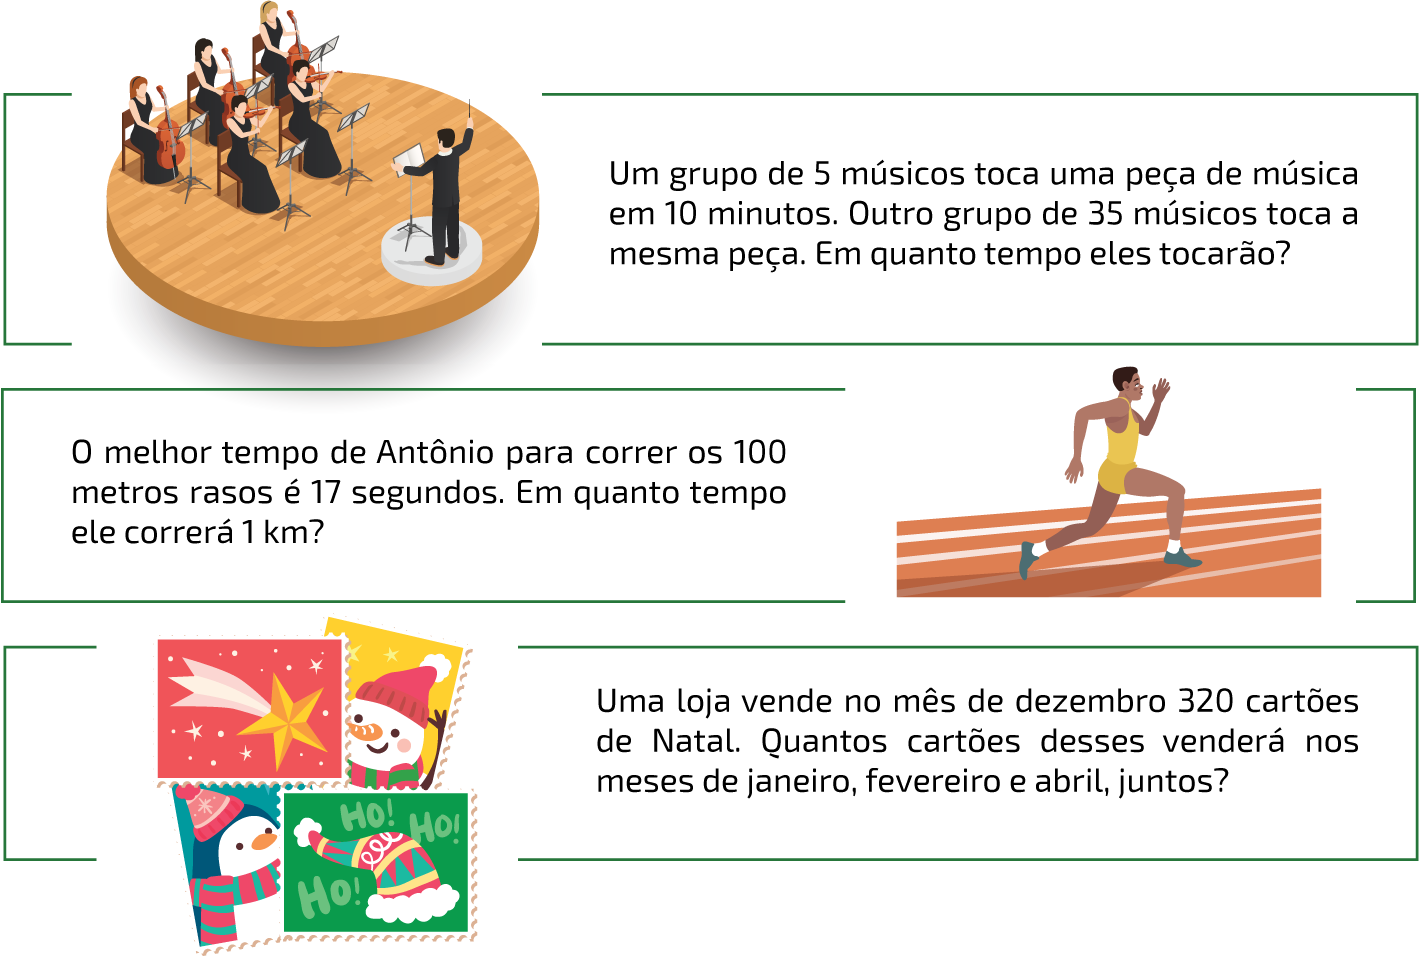
\includegraphics[width=400bp]{naoprop.png}
\end{figure}


Os três problemas acima fornecem três informações e propõem que, a partir delas, determinemos uma quarta informação. Esse é o enunciado típico de problemas cujo método de solução é conhecido como “regra de três”. Entretanto, nenhum dos problemas apresentados, como você deve ter percebido, pode ser resolvido aplicando a tal regra. Você consegue imaginar por quê?

Isso se deve ao fato de que as grandezas relacionadas não são proporcionais entre si. Não é verdade que se \(5\) músicos tocam uma peça de música em \(10\) minutos, \(35\) músicos (que é \(7 \times 5\)) tocarão a peça em \(7 \times 10\) minutos, afinal trata-se da mesma música, logo \(35\), \(45\) ou \(179\) músicos tocarão a tal peça nos mesmos \(10\) minutos. Isto é, o tempo de execução não é diretamente proporcional ao número de músicos que executam a música.

\begin{description}
\item[Teorema]
\leavevmode\phantomsection\label{\detokenize{AF107-0:term-grandezas-diretamente-proporcionais}}
Diz-se que \textbf{duas grandezas são diretamente proporcionais} quando elas se correspondem de tal modo que, multiplicando-se uma quantidade de uma delas por um número real, a quantidade correspondente da outra fica multiplicada pelo mesmo número, sempre que os resultados dessas multiplicações fizerem sentido no contexto observado.
\[\begin{array}{ccc}
X\quad &\overline{\quad \quad \quad}& \quad Y \\
k\cdot X \quad &\overline{\quad \quad \quad}& \quad k\cdot Y
\end{array}\]
\end{description}

É muito comum encontrarmos situações no nosso dia a dia em que as grandezas envolvidas são diretamente proporcionais, e você certamente já resolveu muitos problemas, na escola e fora dela, usando a “regra de três”.

\begin{task}{Na piscina}
\label{ativ-na-piscina}

Duas piscinas de 1000 litros cada estão sendo enchidas simultaneamente. A piscina 1 leva 5 horas para ficar completamente cheia e a piscina 2, 8 horas. A cada hora, o volume total de água em cada piscina foi sendo registrado em dois gráficos


\begin{figure}[H]
\centering

\begin{tikzpicture}[scale=1.5, every node/.style={scale=1}]
\tikzstyle{ponto}=[circle, minimum size=3pt, inner sep=0, draw=\currentcolor!80, fill=\currentcolor!80, shift only]
\begin{scope}[yscale=.5]
\draw[lightgray](0,0)grid[xstep=.25,ystep=.25](6,10);
\draw[gray](0,0)grid(6,10);
\draw[thick, ->](0,0)--(6,0)node [below, shift={(-0.55,-0.2)}]{tempo(horas)};
\draw[thick, ->](-0,0)--(0,10);
\node[right, rotate=90]at (-.9,6){capacidade(litros)};
\foreach \x in{0,1, 2, 3, 4, 5}
\node[ponto]at(\x,2*\x){};
\foreach\x in{0,1, 2, 3, 4, 5, 6}
\node[below] at(\x, 0){ \x};
\foreach\y in{100, 200, 300, ..., 1000}
\node[left]at(0,.01*\y){ \y};
\end{scope}
\end{tikzpicture}
\caption{Piscina 1}
\label{piscina1}
\end{figure}
\begin{figure}[H]
\centering

\begin{tikzpicture}[scale=1.5, every node/.style={scale=1}]
\tikzstyle{ponto}=[circle, minimum size=3pt, inner sep=0, draw=\currentcolor!80, fill=\currentcolor!80, shift only]
\begin{scope}[yscale=.5]
\draw[lightgray](0,0)grid[xstep=.25,ystep=.25](8,10);
\draw[gray](0,0)grid(8,10);
\draw[thick, ->](0,0)--(8,0)node [below, shift={(-0.55,-0.3)}]{tempo(horas)};
\draw[thick, ->](-0,0)--(0,10);
\node[right, rotate=90]at (-.9,6){ capacidade(litros)};
\node[ponto]at(0,0){};
\node[ponto]at(1,1.5){};
\node[ponto]at(2,2){};
\node[ponto]at(3,3){};
\node[ponto]at(4,5){};
\node[ponto]at(5,8){};
\node[ponto]at(6,9){};
\node[ponto]at(7,9.5){};
\node[ponto]at(8,10){};
\foreach\x in{0,1, 2, 3, 4, 5, 6, 7, 8}
\node[below] at(\x, 0){\x};
\foreach\y in{100, 200, 300, ..., 1000}
\node[left]at(0,.01*\y){\y};
\end{scope}
\end{tikzpicture}
\caption{Piscina 2}
\label{piscina2}

\end{figure}

\begin{enumerate}
\item {} 
Construa uma tabela com os dados de cada gráfico.

\item {} 
As grandezas volume total de água e tempo de enchimento da piscina 1 são diretamente proporcionais? Explique.

\item {} 
As grandezas volume total de água e tempo de enchimento da piscina 2 são diretamente proporcionais? Explique.

\end{enumerate}
\end{task}

\begin{reflection}

Suponha que os dados numéricos fossem omitidos dos eixos nos dois gráficos. Ainda assim seria possível determinar a proporcionalidade ou não entre as grandezas? Como?
\end{reflection}

\clearpage
\def\currentcolor{session4}
\begin{sugestions}{Para refletir}
{
  Até o presente momento, apenas argumentamos que se duas grandezas são proporcionais então elas se relacionam de maneira que uma delas é uma função linear da outra. Essa reflexão vai no sentido da afirmação recíproca. E ainda faz uma provocação, sem ter o intuito de formalizar, no sentido de intuir que a função inversa de uma função linear é também uma função linear.
}{1}{2}
\end{sugestions}

\arrange{Função Linear}
\label{\detokenize{AF107-1::doc}}\label{\detokenize{AF107-1:organizando-as-ideias-funcao-linear}}
Considere duas grandezas diretamente proporcionais que podem assumir quaisquer valores reais e vamos representá-las pelas letras \(x\) e \(y\). Então, sempre que multiplicarmos \(x\) por qualquer número real \(k\), o valor correspondente da grandeza \(y\) também fica multiplicado pelo mesmo valor. Isto é
\[\begin{array}{ccc}
x\quad &\overline{\quad \quad \quad}& \quad y \\
k\cdot x \quad &\overline{\quad \quad \quad}& \quad k\cdot y
  \end{array}\]
Vamos agora, traduzir a propriedade acima para a linguagem de função. Consideremos que a grandeza \(y\) é expressa como função da grandeza \(x\), isto é, \(y=f(x)\). Vamos supor que quando a variável $x$ vale 1, o valor correspondente de $y$ é $a$, ou seja, $f(1)=a$. Assim, teremos

\[\begin{array}{ccc}
x\quad &\overline{\quad \quad \quad}& \quad f(x) \\
1 \quad &\overline{\quad \quad \quad}& \quad a \\
2 \quad &\overline{\quad \quad \quad}& \quad 2a \\
3 \quad &\overline{\quad \quad \quad}& \quad 3a \\
\vdots \quad &\overline{\quad \quad \quad}& \quad \vdots\\
  \end{array}\]

\begin{observation}
Usando a ``regra de três'' nas duas primeiras linhas fica assim
\[\begin{array}{ccc}
x \quad &\overline{\quad \quad \quad}& \quad f(x)\\
1\quad &\overline{\quad \quad \quad}& \quad a \end{array}\]
O que nos leva a
\[\dfrac x1 = \dfrac {f(x)}a \Longrightarrow f(x) = a\cdot x\]
\end{observation}

Toda função real que pode ser expressa na forma $f(x)=ax$ para algum número real $a$, é chamada de \textbf{função linear}. Neste caso, as grandezas representadas pelas variáveis $x$ e $y=f(x)$ são diretamente proporcionais. O número $a=f(1)$ é chamado de \textbf{constante de proporcionalidade} entre as grandezas.


Na \DUrole{xref,std,std-ref}{Atividade Na piscina} você deve ter percebido que as grandezas relacionadas eram diretamente proporcionais apenas no caso da piscina 1. Naquele caso, a função que fornece o volume de água na piscina em função do tempo é dada por \(V:\{1,2,3,4,5\}\to \mathbb{R}\),   \(V(t)=V(1)\cdot t=200\cdot t\).

\begin{reflection}

Suponha que duas grandezas \(x\) e \(y\) se relacionem de maneira que \(y\) seja uma função linear de \(x\).
\begin{enumerate}
\item {} 
Essas duas grandezas são proporcionais?

\item {} 
Podemos afirmar também que \(x\) é uma função linear de \(y\)?

\end{enumerate}
\end{reflection}

\needspace{.2\textheight}
\def\currentcolor{session2}
\begin{objectives}{Taxa de Câmbio}
{
\begin{itemize}
\item Utilizar a taxa de câmbio fornecida para realizar a conversão do valor dado em moeda estrangeira para o valor correspondente em reais.

\item Obter a partir das informações fornecidas a função linear que converte dólar americano em reais.

\end{itemize}
}{1}{1}
\end{objectives}
\begin{sugestions}{Taxa de Câmbio}
{
\begin{itemize}
\item É bastante provável que no item \titem{c)} os estudantes apresentem o seguinte raciocínio: se 1 dólar americano equivale a R\$ $3{,}20$ reais então $x$ dólares americanos irão corresponder a $y$ reais, isto é, $y=3,20\cdot x$. Em analogia ao que foi feito anteriormente, é importante chamar atenção de que se $y=f(x)$ é a função que fornece a quantia equivalente em reais a x dólares americanos, como as grandezas envolvidas são diretamente proporcionais e $f(1)=3{,}20$, então $f(x)=x\cdot f(1)$ e portanto $f(x)=3{,}20{,}x$.

\item Ainda no item \titem{c)} o questionamente apresentado sobre o domínio da função tem como objetivo levar a uma reflexão de que na prática não faz sentido, por exemplo, converter $\sqrt{5}$ dólares americanaos para reais.
\end{itemize}
}{1}{1}
\end{sugestions}
\begin{answer}{Taxa de Câmbio}
{
\begin{enumerate}

\item A partir da taxa de câmbio fornecida sabemos que 1 dólar americano é equivalente a R\$ $320{,}00$, e portanto, para comprar 100 dólares americanos serão necessários R\$ $320{,}00$. 

\item Como nesse dia 1 euro é equivalente a R\$ $4{,}00$, então será necessário desembolsar R\$ $800{,}00$ para a compra de $200$ euros.

\item Vamos chamar de $y=f(x)$ a função que fornece a quantia equivalente em reais a x dólares americanos. Como as grandezas envolvidas são diretamente proporcionais e $f(1)=3{,}20$ (veja que isso é a tradução, usando a linguagem de função, de que 1 dólar americano equivale a R\$ $3{,}20$), então $f(x)=x\cdot f(1)$ e portanto $f(x)=3{,}20\cdot x$. Como na prática não existem quantias irracionais de dólares americanos e de reais, devemos considerar $f:\Q\rightarrow\Q$.

\item Utilizando a função obtida no item anterior vemos que R\$ $2000,00$ equivalem a $x\displaystyle=\frac{2000}{3}{,}20=625$ reais. Raciocinando de forma análoga obtemos que com R\$ $2000{,}00$ poderão ser adquiridos $\displaystyle\frac{2000}{4}=500$ euros.
\end{enumerate}
}{0}
\end{answer}
\begin{objectives}{Proporcionalidade na construção de retângulos}
{
\begin{itemize}
\item Levar o estudante a relacionar os conceitos de proporcionalidade e semelhança de figuras e função linear.

\item Construir retângulos que sejam semelhantes a um retângulo dado.

\end{itemize}
}{1}{1}
\end{objectives}
\clearmargin
\marginpar{\vspace{.5em}}
\begin{answer}{Proporcionalidade na construção de retângulos}
{
\begin{enumerate}
\item Não, pois a medida da base dobrou e a altura se manteve.

\item $3$, pois se a medida da base dobrou a altura deve dobrar $1{,}5\cdot2=3$. Os retângulos se relacionam por meio da função linear $f(x)=2\cdot x$.

\item $2{,}5$, pois em todos os retângulos a razão de semelhança, entre a base e a altura é de $12$, portando a altura deve ser a metade da base. Neste caso os retângulos se relacionam por meio da função linear $f(x)=53\cdot x$.

\item $8$, pelo mesmo motivo citado anteriormente, a base deve ser o dobro a altura.

\item Não, pois a razão entre base e altura não é de $12$.

\item $\sqrt{33}$, pois a altura de um triângulo equilátero de lado $3$ é $\frac{3\sqrt{33}}{2}$, ao assumir essa medida como altura do retângulo, sua base deve ser o dobro dessa medida.

\end{enumerate}
}{1}
\end{answer}
\clearmargin
\begin{objectives}{Qual é a área?}
{
\begin{itemize}
\item Em um círculo dado, reconhecer a relação de dependência entre a medida do ângulo central e a medida da área do setor circular.

\item Inferir que a medida da área do setor é diretamente proporcional a medida do ângulo central.

\item Determinar a medida da área do setor circular dada a medida do ângulo central e vice-versa.

\end{itemize}
}{1}{1}
\end{objectives}
\marginpar{\vspace{-1em}}
\begin{sugestions}{Qual é a área?}
{
\begin{itemize}
\item Nos dois primeiros itens procure incentivar os alunos a resolver o problema utilizando apenas processos mentais, ou ao menos na hora de discutir a solução, utilize argumentações que valorizem a estimativa, tais como:

\begin{itemize}
\item Como $\frac{1}{4}$ de $20$ é $5$, e $14$ é um valor um pouco menor que $34$ de $20$ então o setor circular de área $14$ tem que ser menor do que $34$ do círculo.

\item Ao analisar as opções descartamos a opção “2” por ser uma região menor que $34$ da área do círculo, descartamos também a opção “3” por se tratar de um valor entre $15$ e $20$ mais próximo de $15$, logo a resposta correta está representada pela opção “1”.
\end{itemize}

\item Nos itens \titem{c)} e \titem{d)}, discuta com a turma a importância de ter sido apresentado a medida do ângulo.
\end{itemize}
}{1}{1}
\end{sugestions}
\begin{answer}{Qual é a área?}
{
\begin{enumerate}\setcounter{enumi}{4}
\item 2)
\item 1)
\item Uma possível resposta seria: sendo a área total do círculo igual a $20$, então $14$ do círculo equivale a uma área 5. No entanto, como as áreas destacadas nos itens apresentados estão muito próximas esse critério não nos permite concluir com exatidão qual seria a resposta correta, que no caso é o item 2).
\item 2)
\end{enumerate}
}{1}
\end{answer}
\clearmargin
\begin{answer}{Qual é a área}
{
  \begin{enumerate}\setcounter{enumi}{4}
  \item Fazendo uma regra de três, item 1).
  \item $S:[0,360]\rightarrow\R$ em que $S(x)=\frac{x}{18}$
  \end{enumerate}
}{1}
\end{answer}

\practice{Função Linear}
\label{\detokenize{AF107-1:praticando}}

\begin{task}{Taxa de câmbio}
\label{ativ-cambio}



Segundo o \href{http://www.bcb.gov.br/pre/bc\_atende/port/taxCam.asp}{site do Banco Central do Brasil}, a \emph{taxa de câmbio} é o preço de uma moeda estrangeira medido em unidades ou frações (centavos) da moeda nacional. Em um determinado dia as taxas de câmbio do dólar americano e do euro eram respectivamente R\$ $3{,}20$ e R\$ $4{,}00$.
\begin{enumerate}
\item {} 
Nesse mesmo dia você deseja comprar \(100\) dólares. Qual seria o valor em reais necessário para realizar essa compra?

\item {} 
Para adquirir nesse mesmo dia \(200\) euros, qual o valor em reais deverá ser desembolsado?

\item {} 
A partir da taxa praticada nesse dia, apresente uma função que converta dólar americano para reais. Qual o conjunto domínio mais adequado a ser considerado para essa função? Justifique.

\item {} 
Com a taxa de câmbio que está sendo praticada nesse dia, quantos dólares americanos podem ser comprados com R\$ $2000{,}00$. Com os mesmos R\$ $2000{,}00$, quantos euros podem ser adquiridos?

\end{enumerate}
\end{task}



\begin{task}{Proporcionalidade na construção de retângulos}
\label{ativ-prop-retangulo}

Considere o retângulo \(R\) abaixo, de lados \(3\) e \(1{,}5\), e responda as questões propostas.

\begin{figure}[H]
\centering

\begin{tikzpicture}
\tikzstyle{ponto}=[circle, minimum size=2pt, inner sep=0, draw=black, fill=black, shift only]
\draw[thick,black,fill=\currentcolor!80] (0.,0.) -- (3.,0.) -- (3.,1.5) -- (0.,1.5) -- cycle;
\draw (0.2,0.) -- (0.2,0.2) -- (0.,0.2) -- (0.,0.);
\draw (0.,1.3) -- (0.2,1.3) -- (0.2,1.5) -- (0.,1.5);
\draw (2.8,1.5) -- (2.8,1.3) -- (3.,1.3) -- (3.,1.5);
\draw(3.,0.2) -- (2.8,0.2) -- (2.8,0.) -- (3.,0.);
\node[ponto]at(0,0){};
\node[ponto]at(3,0){};
\node[ponto]at(3,1.5){};
\node[ponto]at(0,1.5){};
\node[below ]at(0,0){$$};
\node[below ]at(3,0){$$};
\node[above ]at(3,1.5){$$};
\node[above ]at(0,1.5){$$};
\node[above]at(1.7,-.7){$3$};
\node[right]at(3,.75){$1{,}5$};
\end{tikzpicture}

\end{figure}

\begin{enumerate}
\item {} 
Observe o retângulo da figura a seguir e determine se ele é semelhante ou não ao retângulo \(R\).

\begin{figure}[H]
\centering

\begin{tikzpicture}
\tikzstyle{ponto}=[circle, minimum size=2pt, inner sep=0, draw=black, fill=black, shift only]
\draw[thick,black,fill=\currentcolor!80] (0.,0.) -- (6.,0.) -- (6.,1) -- (0.,1.)-- cycle;
\draw (0.2,0.) -- (0.2,0.2) -- (0.,0.2) -- (0.,0.);
\draw (0.,.8) -- (0.2,.8) -- (0.2,1) -- (0.,1);
\draw (5.8,1) -- (5.8,.8) -- (6.,.8) -- (6.,1);
\draw(6.,0.2) -- (5.8,0.2) -- (5.8,0.) -- (6.,0.);
\node[ponto]at(0,0){};
\node[ponto]at(6,0){};
\node[ponto]at(6,1){};
\node[ponto]at(0,1){};
\node[below ]at(0,0){$$};
\node[below ]at(6,0){$$};
\node[above ]at(6,1){$$};
\node[above ]at(0,1){$$};
\node[above]at(3,-.7){$6$};
\node[right]at(6,.5){$1{,}5$};
\end{tikzpicture}

\end{figure}

\item {} 
Na figura a seguir temos a medida base de um retângulo em destaque, qual deve ser a medida de sua altura para que o retângulo gerado seja semelhante a \(R\)? Qual a função linear que relaciona esses dois retângulos?

\begin{figure}[H]
\centering


\begin{tikzpicture}
\tikzstyle{ponto}=[circle, minimum size=2pt, inner sep=0, draw=black, fill=black, shift only]
\fill[bottom color=\currentcolor!80,top color =white] (0.,0.) -- (6.,0.) -- (6.,.5) -- (0.,.5) -- cycle;
\draw (0.2,0.) -- (0.2,0.2) -- (0.,0.2) -- (0.,0.);
\draw(6.,0.2) -- (5.8,0.2) -- (5.8,0.) -- (6.,0.);
\draw(0.,.5)--(0.,0.) -- (6.,0.) -- (6.,.5);
\node[ponto]at(0,0){};
\draw[fill](0,.6)circle(.5pt);
\draw[fill](0,.7)circle(.5pt);
\draw[fill](0,.8)circle(.5pt);
\node[ponto]at(6,0){};
\draw[fill](6,.6)circle(.5pt);
\draw[fill](6,.7)circle(.5pt);
\draw[fill](6,.8)circle(.5pt);
\node[below ]at(0,0){$$};
\node[below ]at(6,0){$$};
\node[above ]at(6,1.5){$$};
\node[above ]at(0,1.5){$$};
\node[above]at(3,-.7){$6$};
\end{tikzpicture}

\end{figure}
\item {} 
Seguindo a mesma ideia do item anterior, qual deve ser a medida da altura desse novo retângulo de base \(5\), para que ele seja semelhante a \(R\)? E neste caso, qual a função linear entre os retângulos?

\begin{figure}[H]
\centering


\begin{tikzpicture}
\tikzstyle{ponto}=[circle, minimum size=2pt, inner sep=0,   draw=black, fill=black, shift only]
\fill[bottom color=\currentcolor!80,top color =white] (0.,0.) -- (5.,0.) -- (5.,.5) -- (0.,.5) -- cycle;
\draw (0.2,0.) -- (0.2,0.2) -- (0.,0.2) -- (0.,0.);
\draw(5.,0.2) -- (4.8,0.2) -- (4.8,0.) -- (5.,0.);
\draw(0.,.5)--(0.,0.) -- (5.,0.) -- (5.,.5);
\node[ponto]at(0,0){};
\draw[fill](0,.6)circle(.5pt);
\draw[fill](0,.7)circle(.5pt);
\draw[fill](0,.8)circle(.5pt);
\node[ponto]at(5,0){};
\draw[fill](5,.6)circle(.5pt);
\draw[fill](5,.7)circle(.5pt);
\draw[fill](5,.8)circle(.5pt);
\node[below ]at(0,0){$$};
\node[below ]at(5,0){$$};
\node[above ]at(5,1.5){$$};
\node[above ]at(0,1.5){$$};
\node[above]at(2.5,-.7){$5$};
\end{tikzpicture}

\end{figure}
\item {} 
Já na figura a seguir, apresentamos um retângulo de altura \(4\), qual deve ser a medida da base desse novo retângulo, para que ele seja semelhante a \(R\)?

\begin{figure}[H]
\centering

\begin{tikzpicture}
\tikzstyle{ponto}=[circle, minimum size=2pt, inner sep=0, draw=black, fill=black, shift only]
\fill[left color = white, right color =\currentcolor!80,] (2.,0.) -- (3.,0.) -- (3.,2.5) -- (2.,2.5) -- cycle;
\draw[thick] (2.,0.) -- (3.,0.) -- (3.,2.5) -- (2.,2.5) ;
\draw (2.8,2.5) -- (2.8,2.3) -- (3.,2.3) -- (3.,2.5);
\draw(3.,0.2) -- (2.8,0.2) -- (2.8,0.) -- (3.,0.);
\node[ponto]at(0,0){};
\node[ponto]at(3,0){};
\node[ponto]at(3,2.5){};
\node[ponto]at(0,2.5){};
\node[below ]at(0,0){$$};
\node[below ]at(3,0){$$};
\node[above ]at(3,2.5){$$};
\node[above ]at(0,2.5){$$};
\node[right]at(3,1.25){$4$};
\draw[fill](1.7,0)circle(.5pt);
\draw[fill](1.8,0)circle(.5pt);
\draw[fill](1.9,0)circle(.5pt);
\draw[fill](1.7,2.5)circle(.5pt);
\draw[fill](1.8,2.5)circle(.5pt);
\draw[fill](1.9,2.5)circle(.5pt);
\end{tikzpicture}

\end{figure}
\item {} 
Na figura a seguir, apresentamos um retângulo cuja base tem a mesma medida da base de \(R\) (igual a \(3\)), e cuja altura coincide com a de um triângulo equilátero de lado medindo \(3\). Esse retângulo é semelhante a \(R\)?

\begin{figure}[H]
\centering


\begin{tikzpicture}
\tikzstyle{ponto}=[circle, minimum size=2pt, inner sep=0, draw=black, fill=black, shift only]
\draw[fill=\currentcolor!80,very thick](0,0)--(4,0)--(4,3.46)--(0,3.46)--cycle;
\draw[fill=terciario,very thick](0,0)--(4,0)--(2,3.46)--cycle;
\node[ponto]at(0,0){};
\node[ponto]at(4,0){};
\node[ponto]at(4,3.46){};
\node[ponto]at(0,3.46){};
\node[ponto]at(2,3.46){};
\node[below]at(0,0){$$};
\node[below]at(4,0){$$};
\node[above]at(4,3.46){$$};
\node[above]at(0,3.46){$$};
\node[above]at(2,3.46){$$};
\node[above]at(2,-.8){$3$};
\end{tikzpicture}

\end{figure}
\item {} 
Se utlizarmos a altura do retângulo da figura anterior na construção de um novo retângulo, qual deve ser a medida de sua base para que seja semelhante a \(R\)?

\end{enumerate}
\end{task}


\begin{task}{Qual é a área?}
\label{ativ-qual-area}

Caso tenha disponibilidade, sugerimos o uso da construção GeoGebra disponível \href{https://www.geogebra.org/m/Xjjym4e7}{neste link}, que é a versão eletrônica dessa atividade.

\begin{figure}[H]
\centering

\noindent\includegraphics[width=100bp]{{codigo}.png}
\end{figure}



\begin{enumerate}
\item {}
Cada círculo representado a seguir tem área total \(20\). Um   dos setores circulares destacados em verde nesses círculos tem área \(14\). Qual é esse setor?

\begin{figure}[H]
\centering


  \begin{tikzpicture}
    \draw(0,0)circle(1);
    \draw[fill=\currentcolor!80] (1,0)--(0,0) --(210:1) arc (210:0:1);
    \node at(-1,1){(a)};
\end{tikzpicture}\quad\quad\quad
 \begin{tikzpicture}
    \draw(0,0)circle(1);
    \draw[fill=\currentcolor!80] (1,0)--(0,0) --(250:1) arc (250:0:1);
    \node at(-1,1){(b)};
 \end{tikzpicture}\quad\quad\quad
      \begin{tikzpicture}
    \draw(0,0)circle(1);
    \draw[fill=\currentcolor!80] (1,0)--(0,0) --(270:1) arc (270:0:1);
    \node at(-1,1){(c)};
 \end{tikzpicture}
\end{figure}

\item{}
Agora, um dos setores circulares em verde tem área \(18\). Qual é esse setor?

\begin{figure}[H]
\centering


\begin{tikzpicture}
  \draw(0,0)circle(1);
  \draw[fill=\currentcolor!80] (1,0)--(0,0) --(330:1) arc (330:0:1);
  \node at(-1,1){(a)};
 \end{tikzpicture}\quad\quad\quad
      \begin{tikzpicture}
  \draw(0,0)circle(1);
  \draw[fill=\currentcolor!80] (1,0)--(0,0) --(250:1) arc (250:0:1);
  \node at(-1,1){(b)};
 \end{tikzpicture}\quad\quad\quad
      \begin{tikzpicture}
  \draw(0,0)circle(1);
  \draw[fill=\currentcolor!80] (1,0)--(0,0) --(300:1) arc (300:0:1);
  \node at(-1,1){(c)};
\end{tikzpicture}

\end{figure}

 \item{}
Explique a estratégia matemática que você utilizou para resolver os itens anteriores? Dentre os setores circulares apresentados a seguir, um deles tem área \(7\). Aplique sua estratégia para determinar qual é esse setor.

\begin{figure}[H]
\centering


 \begin{tikzpicture}

   \draw(0,0)circle(1);
   \draw[fill=\currentcolor!80] (1,0)--(0,0) --(110:1) arc (110:0:1);
   \node at(-1,1){(a)};
 \end{tikzpicture}\quad\quad\quad
      \begin{tikzpicture}
        \draw(0,0)circle(1);\draw[fill=\currentcolor!80] (1,0)--(0,0) --(126:1) arc (126:0:1);\node at((-1,1){(b)};
         \end{tikzpicture}\quad\quad\quad
      \begin{tikzpicture}
        \draw(0,0)circle(1);
        \draw[fill=\currentcolor!80] (1,0)--(0,0) --(142:1) arc (142:0:1);
        \node at(-1,1){(c)};
      \end{tikzpicture}
 \end{figure}
      
\item{}
Possivelmente você encontrou alguma dificuldade para determinar a resposta correta no item anterior. Que tal acrescentarmos uma informação a mais para ajudar na decisão?

\begin{figure}[H]
\centering


\begin{tikzpicture}
  \draw(0,0)circle(1);
  \draw[fill=\currentcolor!80] (1,0)--(0,0) --(110:1) arc (110:0:1);
  \node at(-1,1){(a)};
  \draw[atento] (.2,0) arc (0:110:.2);
  \node at(.4,.3){\tiny $ 110^\circ$};
   \end{tikzpicture}\quad\quad\quad
      \begin{tikzpicture}
        \draw(0,0)circle(1);
        \draw[fill=\currentcolor!80] (1,0)--(0,0) --(126:1) arc (126:0:1);
        \node at(-1,1){(b)};\draw[atento] (.2,0) arc (0:126:.2);
        \node at(.4,.3){\tiny $126^\circ$};
 \end{tikzpicture}\quad\quad\quad
      \begin{tikzpicture}
        \draw(0,0)circle(1);
        \draw[fill=\currentcolor!80] (1,0)--(0,0) --(142:1) arc (142:0:1);
        \node at(-1,1){(c)};
        \draw[atento] (.2,0) arc (0:142:.2);
        \node at(.4,.3){\tiny $ 142^\circ$};
 \end{tikzpicture}
 \end{figure}

\item{}
E agora? Como você usou a medida do ângulo que determina o setor circular para ajudar no cálculo da área? Vamos fazer mais uma vez! Um dos setores apresentados a seguir tem área \(4\). Determine esse setor.

\begin{figure}[H]
\centering


 \begin{tikzpicture}
\draw(0,0)circle(1);\draw[fill=\currentcolor!80] (1,0)--(0,0) --(72:1) arc (72:0:1);\node at(-1,1){(a)}; \draw[atento] (.2,0) arc (0:72:.2);\node at(.4,.2){\tiny $ 72^\circ$}; \end{tikzpicture}\quad\quad\quad
      \begin{tikzpicture}
\draw(0,0)circle(1);\draw[fill=\currentcolor!80] (1,0)--(0,0) --(60:1) arc (60:0:1);\node at(-1,1){(b)};\draw[atento] (.2,0) arc (0:60:.2);\node at(.5,.2){\tiny $ 60^\circ$}; \end{tikzpicture}\quad\quad\quad
      \begin{tikzpicture}
\draw(0,0)circle(1);\draw[fill=\currentcolor!80] (1,0)--(0,0) --(45:1) arc (45:0:1);\node at(-1,1){(c)};\draw[atento] (.2,0) arc (0:45:.2);\node at(.5,.2){\tiny $ 45^\circ$};
 \end{tikzpicture}%\label{fig-setor5}
\end{figure}

\item{}
Determine a função que relaciona a área do setor circular com o seu ângulo central, especificando seu domínio.

\end{enumerate}
\end{task}

\begin{reflection}

Em uma circunferência, podemos relacionar a área \(A\) e o raio \(r\) por meio da função\linebreak \(A(r)=\pi r^2\). Aumentando o raio da circunferência, sua área também aumenta. Isso nos indica que a função \(A\) é crescente. Reflita um pouco e responda: Essa função é linear? Ou seja, a área de um círculo é proporcional ao seu raio?

\textbf{Pense no seguinte caso:} A área de um círculo de raio \(2r\) é igual ao dobro da área de um círculo de raio \(r\)? Ou ainda, é possível encontrar um número real (fixo) tal que \(A(r)=k\cdot r\)?


\begin{figure}[H]
\centering

\begin{tikzpicture}
\fill[\currentcolor!80](-2,0)circle(2cm);
\node[right]at(0.2,0){\Huge =};
\fill[\currentcolor!80](2,0)circle(1cm);
\node[right]at(3.2,0){\Huge +};
\fill[\currentcolor!80](5,0)circle(1cm);
\node[right]at(6.2,0){\Huge ?};
\draw(-2,0)--+(50:2);
\node[left]at(-1.4,.8){$2r$};
\draw(2,0)--+(50:1);
\node[left]at(2.4,.5){$r$};
\draw(5,0)--+(50:1);
\node[left]at(5.4,.5){$r$};
\end{tikzpicture}

\end{figure}
\end{reflection}

\clearpage
\def\currentcolor{session1}
\begin{objectives}{Teor de álcool sanguíneo}
{
\begin{itemize}
\item Conjecturar que taxa de variação média de uma função linear qualquer é a mesma para qualquer intervalo.
\end{itemize}
}{1}{1}
\end{objectives}
\begin{sugestions}{Teor de álcool sanguíneo}
{
\begin{itemize}
\item A atividade aborda assuntos relacionados a temas transversais, como saúde e consumo de álcool. Sugerimos que procure fazer um trabalho colaborativo com os professores de Biologia, Química e de Geografia para ampliar a discussão com os alunos em questões como os processos bioquímicos do metabolismo do álcool, ou mesmo em questões sobre o a relação entre álcool e direção. No site referenciado há informações adicionais que podem enriquecer a discussão.

\item Caso necessário, faça uma revisão sobre taxa de variação média, vista no capítulo de funções.
\end{itemize}
}{1}{1}
\end{sugestions}
\begin{answer}{Teor de álcool sanguíneo}
{
\begin{enumerate}
\item \adjustbox{valign=t}
{
\begin{tabular}{|>{$}c<{$}|>{$}c<{$}|>{$}c<{$}|}
\hline
\tmat{\bm{x}} & \tmat{\bm{h(x)}} & \tmat{\bm{m(x)}} \tabularnewline
\hline
0 & 0 & 0 \tabularnewline
\hline
1 & 0{,}0205 & 0{,}3075 \tabularnewline
\hline
2 & 0{,}041 & 0{,}615 \tabularnewline
\hline
3 & 0{,}615 & 0{,}9225 \tabularnewline
\hline
4 & 0{,}082 & 1{,}23 \tabularnewline
\hline
5 & 0{,}1025 &1{,}5375 \tabularnewline
\hline
\end{tabular}

}

\item 
\begin{enumerate}
\item $0{,}0205$
\item $0{,}0205$
\item $0{,}0205$
\end{enumerate}
\item
\begin{enumerate}
\item $0{,}3075$
\item $0{,}3075$
\item $0{,}3075$
\end{enumerate}

\item A conjectura é que a taxa de variação média de uma função linear qualquer deve ser constante.
\end{enumerate}
}{1}
\end{answer}
\cleardoublepage
\begin{objectives}{Câmara frigorífica}
{
\begin{enumerate}
\item Perceber com o auxílio da representação gráfica a relação entre taxa de variação média negativa e função linear decrescente.
\end{enumerate}
}{1}{2}
\end{objectives}
\begin{sugestions}{Câmara frigorífica}
{
É possível que os estudantes utilizem regra de três para responder as questões propostas no item a). A seguir iremos construir a representação gráfica da função linear, por isso é importante fazer a conexão da regra de três com sua interpretação geométrica, destacando o uso da semelhança de triângulos.

\begin{figure}[H]
\centering

\begin{tikzpicture}[yscale=.5]
\tikzstyle{ponto}=[circle, minimum size=3pt, inner sep=0,    draw=black, fill=black, shift only]
\draw[->, thick](-1,0)--(5,0);
\draw[->, thick](0,-13)--(0,2);
\draw[\currentcolor!80, thick](0,0)--(4,-12);
\draw[dashed](0,-12)--(4,-12)--(4,0);
\node[ponto]at (0,0){};
\node[ponto]at (4,-12){};
\node[above,rotate=90] at(-1,-10){Temperatura $^\circ$C};
\node[above] at(5,0){Tempo (h)};
\node[above] at(4,0){8};
\node[left] at(0,-12){$-24$};
\node[above] at(2,0){$t$};
\node[left] at(0,-6){$f(t)$};
\draw[dashed](2,0)--(2,-6)--(0,-6);
\node[ponto]at (2,-6){};
\end{tikzpicture}
\end{figure}
}{1}{2}
\end{sugestions}
\begin{answer}{Câmara frigorífica}
{
\begin{enumerate}
\item Após 1 hora desde a primeira observaço, a temperatura será de $-3^{\circ}$ C. Após 5 horas, a temperatura será de $-15^{\circ}$, e $t$ horas após a primeira observação, a temperatura 'será de $-3t^{\circ}$ C

\item $-3^{\circ}$ C/h

\item $f:[0,8]\rightarrow\R, f(t)=-3t$ é uma função decrescente, pois à medida que o tempo aumenta, a temperatura correspendente diminui. Ou ainda, para quaisquer tempos $t_1$ e $t_2$ tais que $t_1<t_2$ tem-se que $-3t_1>-3t_2$, isto é $f(t_1)>f(t_2)$.

\item A expressão da função é $f(t)=1{,}5\cdot t$. É uma função crescente, pois à medida que o tempo aumenta, a temperatura correspendente também aumenta.

\begin{tikzpicture}
\tikzstyle{ponto}=[circle, minimum size=2pt, inner sep=0, draw=black, fill=black, shift only]
\draw[->, thick](-1,0)--(6,0)node[above, xshift=-.5cm]{Tempo (h)};
\draw[->, thick](0,-1)--(0,7)node[left,xshift=-.7cm, rotate=90]{Temperatura ($^\circ$C)};
\draw[\currentcolor!80, domain=0:4.4]plot(\x, 1.5*\x);
\node[below]at (1,0){1};
\node[below]at (4,0){8};
\node[left]at (0,1.5){1.5};
\node[left]at (0,6){12};
\draw[dashed](0,1.5)--(1,1.5)--(1,0);
\draw[dashed](0,6)--(4,6)--(4,0);
\end{tikzpicture}

\item Quando a taxa de variação média de uma função linear é um número real \textit{positivo}, a função é \textit{crescente} e quando a taxa é um número real \textit{negativo}, a função é \textit{descrescente}.
\end{enumerate}
}{0}
\end{answer}
\clearmargin
\begin{objectives}{Hora de carregar o celular}
{
\begin{itemize}
\item Perceber, a partir da taxa de variação média constante, que o gráfico de uma função linear está contido em uma reta.
\end{itemize}
}{1}{1}
\end{objectives}
\begin{sugestions}{Hora de carregar o celular}
{
\begin{itemize}
\item No item d) é possível que os estudantes façam direto a “regra de três”; o que está correto. Contudo, peça para que justifiquem o procedimento usando alguma justificativa geométrica envolvendo os pontos do gráfico. A ideia é que, nesse item eles percebam os triângulos semelhantes que podem ser considerados para a solução.
\end{itemize}
}{1}{1}
\end{sugestions}
\begin{answer}{Hora de carregar o celular}
{
\begin{enumerate}

\item \adjustbox{valign=t}
{
\begin{tabular}{|c|c|}
\hline
\tcolor{$t$ (min)} & \tcolor{Porcentagem de recarga} \\
\hline
0 & 0 \\
25 & 20 \\
\hline
50 & 40 \\
\hline 
75 & 60 \\
\hline 
100 & 80 \\
\hline
125 & 100 \\
\hline
\end{tabular}
}

\item\adjustbox{valign=t}
{
\begin{tikzpicture}
\tikzstyle{ponto}=[circle, minimum size=2pt, inner sep=0, draw=black, fill=black, shift only]         
\draw[->, thick](-1,0)--(6,0) node[below right]{tempo(min)};
\draw[->, thick](0,-1)--(0,6);
\foreach \x/\y in{25/20, 50/40, 75/60, 100/80, 125/100}
\node[ponto]at(.04*\x, .05*\y){};
\foreach \x/\y in{25/20, 50/40, 75/60, 100/80, 125/100}
\draw[dashed](.04*\x,0)--(.04*\x,.05*\y)--(0,.05*\y) node[left]{\y} node[below] at(.04*\x,0){\x};
\node[ponto]at(0,0){};
\node[below left]at(0,0){0};
\end{tikzpicture}
}

\item A partir da representação dos pontos no plano cartesiano pode-se concluir, usando semelhança de triângulos, que se em 25 minutos a carga na bateria é de $20\%$ então em 40 minutos a carga será de $32\%$.

\item $f(t)=\displaystyle\frac{45}{t}=0{,}8t$, com domínio sendo o conjunto ${0,1,2,...,125}$ e a imagem o conjunto ${0,1,2,...,100}$.

\item A bateria carrega a uma taxa de 0{,}8\% a cada minuto, isto é, $0{,}8$/min.
\end{enumerate}
}{0}
\end{answer}

\clearpage
\explore{Taxa de Variação Média}
% \label{\detokenize{AF107-2:explorando-taxa-de-variacao-media}}\label{\detokenize{AF107-2::doc}}
\phantom{M}
\vspace{-1em}
\vspace{-2\parskip}
\begin{task}{Teor de álcool sanguíneo}
\label{ativ-alcool}

De acordo com o site \href{https://pt.wikihow.com/Calcular-o-N\%C3\%ADvel-de-\%C3\%81lcool-no-Sangue}{wikiHow} o Teor Alcoólico Sanguíneo, ou TAS, é a medida da proporção de álcool no sangue de uma pessoa. Um TAS de \(0{,}08\) indica que há \(80\) mg de álcool por \(100\) ml de sangue. O álcool é absorvido de forma diferente pelos homens e pelas mulheres. O corpo masculino geralmente tem mais água (\(61\%\) \emph{versus} \(52\%\)) e, portanto, dilui melhor o álcool, gerando TAS mais baixos.

O TAS é proporcional ao número de doses de bebida consumidas, de maneira que para um homem de \(75\) kg, a função linear \(h(x)\) que relaciona o TAS com o número de doses \(x\) de bebida é dada pela expressão
\begin{equation*}
\begin{split}h(x)=0{,}0205 \cdot x.\end{split}
\end{equation*}
Para uma mulher que pesa \(60\) kg, a mesma relação é dada pela função linear
\begin{equation*}
\begin{split}m(x)=0{,}0307 \cdot x.\end{split}
\end{equation*}\begin{enumerate}
\item {} 
Complete a tabela a seguir que relaciona os valores de \(h(x)\) e de \(m(x)\) correspondentes a valores inteiros de \(x\), de \(0\) a \(5\).

\begin{table}[H]
\centering
\begin{tabular}{|l|c|c|}
\hline
\tcolor{\(\bm{x}\)} & \tcolor{\(\bm{h(x)}\)} & \tcolor{\(\bm{m(x)}\)} \\
\hline
0 & & \\
\hline
1 & & \\
\hline
2 & & \\
\hline
3 & & \\
\hline
4 & & \\
\hline
5 & & \\
\hline
\end{tabular}
\end{table}

\item {} 
Calcule, para a função \(h(x)\), as taxas de variação médias nos seguintes intervalos de valores de \(x\):

\begin{enumerate}
\item entre \(x=0\) e \(x=1\);

\item entre \(x=1\) e \(x=3\);

\item entre \(x=2\) e \(x=5\);
\end{enumerate}

\item {} 
Repita o item anterior para a função \(m(x)\) nos intervalos:

\begin{enumerate}
\item entre \(x=2\) e \(x=3\);

\item entre \(x=1\) e \(x=4\);

\item entre \(x=0\) e \(x=5\);
\end{enumerate}

\item {} 
A partir dos itens anteriores, faça uma conjectura sobre as taxas de variação médias de uma função linear qualquer.

\end{enumerate}
\end{task}

\begin{task}{Câmara frigorífica}
\label{ativ-camara}


Uma câmara frigorífica está programada para diminuir sua temperatura segundo uma taxa constante em \(^\circ\)C por hora. Na primeira observação constata-se que ela está a \(0^\circ\) C. Após \(8\) horas, realiza-se uma nova observação e seu visor mostra a temperatura de \(-24^\circ\) e também o seguinte gráfico para a evolução da temperatura em função do tempo.

\begin{figure}[H]
\centering

\begin{tikzpicture}[yscale=.6, xscale=1]
\tikzstyle{ponto}=[circle, minimum size=3pt, inner sep=0, draw=black, fill=black, shift only]
\draw(-3,-.05) grid(5,.05);
\draw(-.05,-12) grid(.05,2);
\draw[->, thick](-3,0)--(5,0);
\draw[->, thick](0,-12)--(0,2);
\draw[\currentcolor!80, thick](0,0)--(4,-12);
\draw[dashed](0,-12)--(4,-12)--(4,0);
\node[ponto]at (0,0){};
\node[ponto]at (4,-12){};
\node[above,rotate=90] at(-1,-10){Temperatura $^\circ$C};
\node[above] at(4,0){Tempo (h)};
\foreach\x in{-4, -2, 0, 2, 4, 6, 8}
\node[below left] at (.5*\x, 0){\x};
\foreach \y in{-24, -22, -20, ..., -2}
\node[left]at(0,.5*\y){\y};
\node[left]at(0,1){2};
\node[left]at(0,2){4};
\end{tikzpicture}
\end{figure}
\begin{enumerate}
\item {} 
Qual a temperatura da câmara \(1\) hora após a primeira observação? E \(5\) horas após a primeira observação? E \(t\) horas após a primeira observação?

\item {} 
Qual o valor da taxa (de variação média) constante segundo a qual a temperatura diminui?

\item {} 
Determine a função que relaciona temperatura e tempo nesse contexto, considerando para seu domínio o intervalo de números reais \([0,8]\). Ela é uma função crescente ou decrescente? Por que?

\item {} 
Como seria o gráfico se a temperatura, no mesmo intervalo de tempo, ao invés de diminuir, estivesse aumentando \(1{,}5^\circ\)C/h? Qual seria a expressão da função, nesse caso? Teríamos uma função crescente ou decrescente? Por que?

\item {} 
Complete as lacunas da sentença abaixo para formular uma conjectura que relacione a taxa de variação média da função linear com o crescimento ou decrescimento da função.

“Quando a taxa de variação média de uma função linear é um número real \makebox[6em]{\hrulefill}, a função é \makebox[8em]{\hrulefill} e quando a taxa é um número real \makebox[8em]{\hrulefill}, a função é \makebox[8em]{\hrulefill}.”

\end{enumerate}
\end{task}

\begin{task}{Hora de carregar o celular}
\label{ativ-celular}

\begin{figure}[H]
\centering

\noindent\includegraphics[width=100bp]{{celular}.jpg}
\end{figure}

O tempo total de recarga da bateria (de \(0\%\) a \(100\%\)) de um determinado modelo de telefone celular é  de \(2\) horas e \(5\) minutos. Supondo que o carregamento ocorre segundo uma taxa constante:

\begin{enumerate}
\item {} 
Faça uma tabela que forneça o percentual de carga na bateria a cada \(25\) minutos, a partir de zero.

\item {} 
Represente em um plano cartesiano os pontos da tabela do item anterior.

\item {} 
Descreva uma estratégia que permita, a partir da representação gráfica obtida no item anterior, determinar o percentual de carga na bateria após \(40\) minutos de carregamento.

\item {} 
Determine a função que modela o carregamento desse modelo de telefone, especificando seus domínio e conjunto imagem.

\item {} 
Qual é a taxa de carregamento desse modelo de telefone celular.
\end{enumerate}
\end{task}

\clearpage
\def\currentcolor{session4}
\begin{sugestions}{Para refletir}
{
  Essa ideia será trabalhada mais adiante na seção dedicada a função afim. Por enquanto, deixe que criem suas próprias jutificativas e contra-exemplos
}{1}{2}
\end{sugestions}
\arrange{Taxa de Variação Média}
\label{\detokenize{AF107-2:organizando-as-ideias-taxa-de-variacao-media}}
No capítulo de Taxa de variação, você aprendeu a calcular a taxa de variação média de uma função em um determinado intervalo. É um número expresso em forma de uma razão que fornece diversas informações sobre o comportamento da função no intervalo considerado.

Relembrando, se um intervalo \([x_1,x_2]\) está contido no domínio de uma função \(f\), então a taxa de variação média dessa função nesse intervalo é a razão
\begin{equation*}
\begin{split}\dfrac{f(x_2)-f(x_1)}{x_2-x_1}\end{split}.
\end{equation*}
Como você deve ter percebido na \DUrole{xref,std,std-ref}{Atividade Teor de álcool sanguíneo}, o valor obtido para as taxas de variação médias nos diversos intervalos foi sempre o mesmo para cada função considerada. Essa é uma propriedade importante das funções lineares, que provaremos agora.

Considere uma função linear \(\ell:\mathbb{R}\to\mathbb{R}\), dada por \(\ell(x)=a\cdot x\), e também dois números reais distintos \(x_1<x_2\). A taxa de variação média de \(\ell\) no intervalo  \([x_1,x_2]\) pode ser calculada assim
\begin{equation*}
\begin{split}\dfrac{\ell(x_2)-\ell(x_1)}{x_2-x_1}=\dfrac{a x_2- a x_1}{x_2-x_1}=\dfrac{a(x_2-x_1)}{x_2-x_1}=a.\end{split}
\end{equation*}
Podemos destacar duas coisas sobre a conclusão deste último cálculo:
\begin{itemize}
\item {} 
o valor final para a taxa de variação média não depende dos valores de \(x_1\) e \(x_2\). Isso significa que podemos escolher qualquer intervalo  de números reais e chegaremos ao mesmo resultado.

\item {} 
o resultado coincide com o coeficiente de \(x\) na expressão da função, e também pode ser obtido calculando-se a imagem de \(x=1\). Sendo assim, podemos afirmar que a função \(y=7x\) tem taxa de variação média constante igual a \(7\), enquanto que a função \(y=-\dfrac {3x}5\) tem taxa de variação média constante igual a \(-\dfrac {3}5\).

\end{itemize}

\begin{description}
\item[Teorema]
Toda função linear \(f\) tem taxa de variação média constante igual a \(f(1)\), e pode ser representada pela expressão \(f(x)=f(1)\cdot x\).
\end{description}

\begin{reflection}
É verdade que se uma função tem taxa de variação média constante então ela é uma função linear? Pense em exemplos com taxas de variação médias constantes e verifique se há ou não proporcionalidade nesses casos.
\end{reflection}

Usando essas ideias no contexto da \DUrole{xref,std,std-ref}{Atividade Câmara frigorífica}, podemos afirmar que a expressão da temperatura em função do tempo, mostrada pelo gráfico pode ser dada por \(f(t)=-3t\), uma vez que \(f(1)=-3\). A cada hora a temperatura decresce \(3^\circ\)C, gerando portanto uma função decrescente.

De uma maneira geral, se a taxa de variação média \(a\) de uma função linear é um número real \textbf{negativo}, então essa função é decrescente, pois, para \(a<0\)
\begin{equation*}
\begin{split}x_1<x_2 \Longleftrightarrow ax_1>ax_2 \Longleftrightarrow f(x_1)>f(x_2).\end{split}
\end{equation*}
Por outro lado, se a taxa de variação média \(a\) de uma função linear é um número real \textbf{positivo}, então essa função é crescente, pois, nesse caso \(a>0\) e
\begin{equation*}
\begin{split}x_1<x_2 \Longleftrightarrow ax_1<ax_2 \Longleftrightarrow f(x_1)<f(x_2).\end{split}
\end{equation*}
Vamos agora entender como é a representação gráfica de uma função com taxa de variação média constante. Para isso, consideremos uma função \(f:\mathbb{R}\to\mathbb{R}\) que tenha essa propriedade, isto é, para qualquer intervalo a taxa de variação média de \(f\) neste intervalo é igual a \(a\).

Na figura a seguir, os pontos \(A=(x_1,f(x_1))\) e \(B=(x_2,f(x_2))\) pertencem ao gráfico da função \(f\). O segmento \(BC\) mede \(f(x_2)-f(x_1)\) e o segmento \(AC\) mede \(x_2-x_1\). Dessa forma o quociente \(\dfrac{\overline{BC}}{\overline{AC}}\) é igual à taxa de variação média da função nesse intervalo, e portanto podemos conluir que \(\overline{BC}=a\cdot \overline{AC}\).

\begin{figure}[H]
\centering


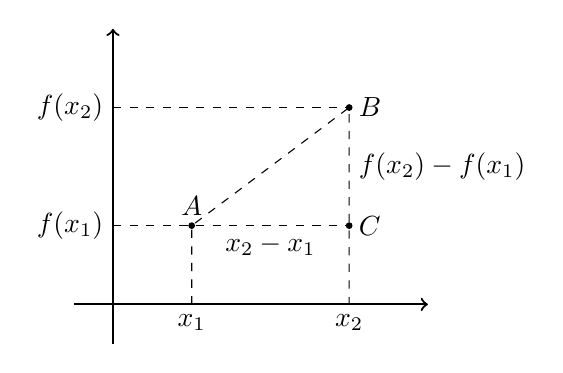
\begin{tikzpicture}
\tikzstyle{ponto}=[circle, minimum size=2pt, inner sep=0, draw=black, fill=black, shift only]
\draw[->, thick](-.5,0)--(4,0);
\draw[->, thick](0,-.5)--(0,3.5);
\draw[dashed](0,1)--(3,1);
\draw[dashed](0,2.5)--(3,2.5);
\draw[dashed](1,0)--(1,1)--(3,2.5)--(3,0);
\node[below] at(1,0){$x_1$};
\node[below] at(3,0){$x_2$};
\node[below] at(2,1){$x_2-x_1$};
\node[right, rotate=0] at(3,1.75){$f(x_2)-f(x_1)$};
\node[left] at(0,1){$f(x_1)$};
\node[left] at(0,2.5){$f(x_2)$};
\node[ponto]at(1,1){};
\node[above]at(1,1){$A$};
\node[ponto]at(3,1){};
\node[right]at(3,1){$C$};
\node[ponto]at(3,2.5){};
\node[right]at(3,2.5){$B$};
\end{tikzpicture}
\end{figure}

\begin{equation*}
\begin{split}\dfrac{\overline{BC}}{\overline{AC}}= \dfrac{f(x_2)-f(x_1)}{x_2-x_1}=a \Longrightarrow \overline{BC}=a\cdot \overline{AC}.\end{split}
\end{equation*}
Por isso, quaisquer dois pontos do gráfico de \(f\), sempre serão extremidades da hipotenusa de um triângulo retângulo cujos catetos são paralelos aos eixos e suas medidas se relacionam conforme a seguinte figura.

\begin{figure}[H]
\centering

\begin{tikzpicture}
\tikzstyle{ponto}=[circle, minimum size=2pt, inner sep=0, draw=black, fill=black, shift only]
\draw[->, thick](-.5,0)--(4,0);
\draw[->, thick](0,-.5)--(0,3.5);
\draw[dashed](1,1)--(3,1);
\draw[dashed](1,1)--(3,2.5)--(3,1);
\node[below] at(2,1){$d$};
\node[right, rotate=0] at(3,1.75){$a\cdot d$};
\node[ponto]at(1,1){};
\node[ponto]at(3,1){};
\node[ponto]at(3,2.5){};
\end{tikzpicture}
\end{figure}

Consideremos agora três pontos do gráfico de \(f\) com os respectivos triângulos retângulos da construção anterior.
\begin{figure}[H]
\centering

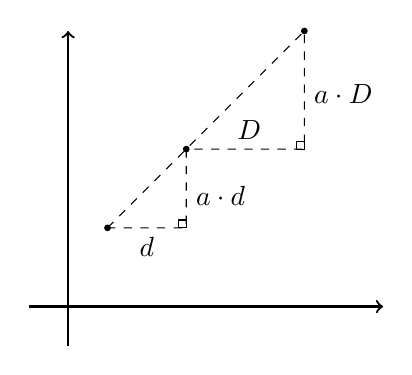
\begin{tikzpicture}
\tikzstyle{ponto}=[circle, minimum size=2pt, inner sep=0, draw=black, fill=black, shift only]
\draw[->, thick](-.5,0)--(4,0);
\draw[->, thick](0,-.5)--(0,3.5);
\draw[dashed](.5,1)--(3,3.5)--(3,2)--(1.5,2)--(1.5,1)--cycle;
\node[ponto]at(.5,1){};
\node[ponto]at(1.5,2){};
\node[ponto]at(3,3.5){};
\node[below]at(1,1){$d$};
\node[right]at(1.5,1.4){$a\cdot d$};
\node[above]at(2.3,2){$D$};
\node[right]at(3,2.7){$a\cdot D$};
\draw(1.5,1)rectangle++(-1mm, 1mm);
\draw(3,2)rectangle++(-1mm, 1mm);
\end{tikzpicture}
\end{figure}
Como os triângulos são semelhantes e têm um ponto em comum, podemos concluir que os três pontos pertencem a uma mesma reta. A conclusão é válida quaisquer que sejam os três pontos considerados, logo acabamos de justificar a seguinte propriedade.

\begin{description}
\item[Teorema]

Se uma função tem taxa de variação média constante então seu gráfico está contido em uma reta.

Em particular, como a função linear tem taxa de variação média constante, seu gráfico está contido em uma reta.
\end{description}


\begin{observation}{Algumas propriedades da função linear}


\begin{itemize}
\item {} 
Sempre que fizer sentido calcular a imagem de \(x=0\), teremos \(f(0)=a \cdot 0 = 0\), isto é, a origem \((0,0)\) do plano cartesiano pertencerá ao gráfico de \(f\). Em qualquer caso, o gráfico de uma função linear está contido em uma reta que passa pela origem (mesmo quando não fizer sentido calcular a imagem de \(x=0\)).

\item {} 
A taxa de variação da função linear \(f(x)=ax\) também pode ser calculada fazendo-se a diferença entre as imagens de dois valores que distam \(1\) entre si da seguinte maneira:

\end{itemize}
\begin{equation*}
\begin{split}f(x+1)-f(x)=a(x+1)-ax=ax+a-ax=a\end{split}
\end{equation*}

\begin{figure}[H]
\centering

\begin{tikzpicture}
\tikzstyle{ponto}=[circle, minimum size=2pt, inner sep=0, draw=black, fill=black, shift only]
\draw[thick,->](-1,0)--(4,0);
\draw[thick,->](0,-1)--(0,4);
\draw[domain=-.5:2, thick, \currentcolor!80]plot(\x,2*\x);
\draw[dashed, thick](.5,0)--(.5,1)--(0,1);
\draw[dashed, thick](1.5,0)--(1.5,3)--(0,3);
\draw[dashed, thick](.5,1)--(1.5,1);
\node[ponto] at(.5,1){};
\node[ponto] at(1.5,3){};
\node[right] at(1.5,2){$a$};
\node[below] at(1,1){$1$};
\node[below] at(1.5,.1){$x+1$};
\node[below] at(.5,0){$x$};
\node[left] at(0,3){$f(x+1)$};
\node[left] at(0,1){$f(x)$};
\end{tikzpicture}
\end{figure}

\begin{itemize}
\item {} 
%Para taxas de variação médias positivas, quanto maior for o valor de \(a\), mais inclinada será a reta que contém o gráfico da função linear associada.
A função linear $f(x)=x$ é chamada \textbf{função identidade}.

\begin{figure}[H]
\centering

\begin{tikzpicture}[scale=0.5, every node/.style={scale=0.7}]

\draw [gray!50](-6.5,-6.5) grid (6.5,6.5);
\draw [->] (-6.5,0) -- (6.5,0);
\draw [->] (0,-6.5) -- (0,6.5);
\foreach \x in {-6,...,-1,1,2,...,6}{
\node [below] at (\x,0) {\x};
\node [left] at (0,\x) {\x};
}

\draw [very thick, \currentcolor!80] (-6.5,-6.5) -- (6.5,6.5);
\node [above left] at (0,0) {0};
\end{tikzpicture}
\end{figure}

\end{itemize}

% \begin{figure}[H]
% \centering

% \noindent\includegraphics[width=400bp]{{aumenta_a}.png}
% \end{figure}

Para uma visualização do comportamento da representação gráfica com taxa de variação média também negativa, sugerimos o uso da construção GeoGebra disponível \href{https://www.geogebra.org/m/FSnzt9vC}{neste link} .

\begin{figure}[H]
\centering

\noindent\includegraphics[width=100bp]{{codigo2_2}.png}
\end{figure}

%\begin{figure}[H]
%\centering
%
%\noindent\includegraphics[width=400bp]{{taxa_linear}.png}
%\end{figure}
\begin{itemize}
\item {} 
Se uma reta contém a origem do plano cartesiano e o ponto \((x_0,y_0)\) com \(x_0\neq 0\), então ela é o gráfico da função linear \(f:\mathbb{R}\to\mathbb{R}\), dada por \(f(x)=ax\), em que \(a=\dfrac{y_0}{x_0}\).

\end{itemize}

Para verificar isso, basta observarmos uma reta nas condições dadas e os dois  triângulos retângulos destacados da figura a seguir a partir da origem e dos pontos \((x_0,y_0)\) e \((x,y)\). Observe que, qualquer que seja o ponto \((x,y)\) escolhido diferente da origem, esses triângulos são semelhantes, portanto,
\begin{equation*}
\begin{split}\dfrac{f(x)}{x}=\dfrac{y_0}{x_0} \Longrightarrow f(x)=\dfrac{y_0}{x_0} \cdot x\end{split}
\end{equation*}

\begin{figure}[H]
\centering

\begin{tikzpicture}
\tikzstyle{ponto}=[circle, minimum size=2pt, inner sep=0, draw=black, fill=black, shift only]
\usetikzlibrary[patterns]
\fill[color=terciario](2,0)--(2,1.5)--(0,0)-- cycle;
\fill[pattern color=secundario, pattern =north east lines](3,0)--(3,2.25)--(0,0)-- cycle;
\draw[dashed](2,0)--(2,1.5)--(0,1.5);
\draw[dashed](3,0)--(3,2.25)--(0,2.25);
\draw[thick, ->](-1.5,0)--(3.5,0);
\draw[thick, ->] (0,-1.5)--(0,3.5);
\draw[thick,\currentcolor!80,domain=-1.5:4]plot(\x,.75*\x);
\node[ponto]at(2, 1.5){};
\node[ponto]at(3, 2.25){};
\node[below] at(2,0){$x$};
\node[below] at(3,0){$x_0$};
\node[left] at(0,1.5){$f(x)$};
\node[left] at(0,2.25){$y_0$};
\end{tikzpicture}

\end{figure}
Assim, por exemplo, a reta que contém a origem e o ponto \((3,8)\) é o gráfico da função \(f(x)=\dfrac 83 x\). Se a reta contém a origem e o ponto \((-5,2)\) ela será o gráfico da função \(g(x)=\dfrac{2}{-5} x=-\dfrac{2}{5}x\).
\begin{figure}[H]
\centering

\begin{tikzpicture}
\tikzstyle{ponto}=[circle, minimum size=2pt, inner sep=0, draw=black, fill=black, shift only]
\draw[thick, ->](-2,0)--(2.5,0);
\draw[thick, ->] (0,-1.5)--(0,3.5);
\draw[thick,\currentcolor!80,samples=100,domain=-.5:1.15]plot(\x, 3*\x);
\draw[dashed](.5,0)--(.5,1.5)--(0,1.5);
\node[ponto]at(.5,1.5){};
\node[right]at(.5,1.5){$(3,8)$};
\node[below]at(.5,0){$3$};
\node[left]at(0,1.5){$8$};
\end{tikzpicture}

\end{figure}
Gráfico da função \(f(x)=\dfrac 83 x\)
\begin{figure}[H]
\centering

\begin{tikzpicture}[scale=1.5]
\tikzstyle{ponto}=[circle, minimum size=2pt, inner sep=0, draw=black, fill=black, shift only]
\draw[thick, ->](-3,0)--(3,0);
\draw[thick, ->] (0,-1.5)--(0,2);
\draw[dashed](-1.5,0)--(-1.5,.5)--(0,.5);
\node[above] at(-1.5,.5){$(-5,2)$};
\node[below] at(-1.5,0){$-5$};
\node[right] at(0,.5){$2$};
\draw[domain=-3:3,thick,\currentcolor!80,samples=100]plot(\x,{-\x/3});
\node[ponto] at(-1.5,.5){};
\end{tikzpicture}
\end{figure}
Gráfico da função \(g(x)=-\dfrac{2}{5}x\).

Concluímos, assim, que toda reta não vertical que contém a origem é o gráfico de uma função linear.
\end{observation}

\clearpage
\def\currentcolor{session2}
\begin{objectives}{Quando trocar o filtro do purificador?}
{
\begin{itemize}
\item Identificar num conjunto de grandezas distintas e apresentadas em um quadro, duas grandezas que atendem as especificações da situação problema.
\item Perceber a relação da razão entre as grandezas com a taxa de variação da função linear.
\item Aplicar os conceitos de função linear com o intuito de resolver a situação problema.
\end{itemize}
}{1}{1}
\end{objectives}
\begin{sugestions}{Quando trocar o filtro do purificador?}
{
\begin{itemize}
\item No item \titem{d)}, explore com seus alunos o motivo pelo qual o resultado é o mesmo em ambos os casos.
\item Utilize o fato que a atividade anterior também aborda o conceito de função linear e faça um comparativo com os gráficos das duas atividades.
\item Se possível, consulte seu diretor ou responsável direto, como anda a troca dos filtros dos bebedouros da sua escola. Caso consiga o manual dos fabricantes, simule a mesma atividade com os dados da realidade de sua escola.
\item Conduza seus estudantes a perceber a diferença entre a resposta do item e) que é uma razão: $9$ litros/dia, e as respostas dadas aos dois itens anteriores em que tratam do consumo em litros para cada intervalo de tempo.
\end{itemize}
}{1}{1}
\end{sugestions}
\clearmargin
\begin{answer}{Quando trocar o filtro do purificador?}
{
\begin{enumerate}
\item Vida útil do elemento filtrante e vazão máxima recomendada.
\item A cada minuto sai 0,75 litro de água do purificador.
\item $0,75\times12=9$ litros.
\item $9$ litros em ambos os casos.
\item $9$ litros.
\item A vida útil do filtro interno, nas condições descritas, será de aproximadamente 14 meses e meio. A troca do filtro interno deverá ser realizada daqui a dois meses e meio.
\item $f(t)=9t$.

\begin{figure}[H]
\centering


\begin{tikzpicture}[yscale=.5,scale=1.25]
\tikzstyle{ponto}=[circle, minimum size=2pt, inner sep=0, draw=black, fill=black, shift only]   
\draw[thick,->](-3,0)--(3,0)node[ right]{$t$};
\draw[thick,->](0,-2)--(0,10)node[right]{$f(t)$};
\draw[lightgray!50](-3,-2) grid[step=.5](3,10);
\draw[gray](-3,-2) grid(3,10);
\foreach \x in { -3, -2,-1}
\node at  (\x ,-.3)  {\x};
\foreach \x in {3, 2,1}
\node at  (\x ,-.3)  {\x};
\foreach \x in { -2,-1}
\node at  (-.3 ,\x)  {\x};
\foreach \x in {1, 2, 3, ..., 10}
\node at  (-.3 ,\x)  {\x};
\draw[domain=-.2:1.1, \currentcolor!80,very thick, samples=100]plot(\x,9*\x);
\end{tikzpicture}
\end{figure}
\end{enumerate}
}{1}
\end{answer}

\practice{Taxa de Variação Média}
\label{\detokenize{AF107-3::doc}}\label{\detokenize{AF107-3:praticando}}

\begin{task}{Quando trocar o filtro do purificador?}
\label{quando-trocar-o-filtro-do-purificador}

Há \(1\) ano você adquiriu um purificador de água com capacidade de refrigeração, e deseja saber quanto tempo falta para realizar a troca do filtro interno. No manual do fabricante do seu purificador, você encontra o seguinte quadro:


\begin{longtable}{|e{3cm}|e{2cm}|e{2cm}|e{2cm}|e{2cm}|e{2cm}|}
\hline\endfirsthead

\tcolor{} & \tcolor{FIT} & \tcolor{FLAT}& \tcolor{PLUS} & \tcolor{SLIM} & \tcolor{STAR} \\
\hline
\makecell{Dimensões \\ Altura \\ Largura \\ Profundidade} &\makecell{ 27cm \\ 29cm \\ 36cm} & \makecell{29cm \\ 36cm \\36cm} & \makecell{40cm \\ 30cm \\ 45cm} & \makecell{36cm \\ 25cm \\ 41cm} & \makecell{40cm \\ 30cm \\ 36cm}\\
\hline
Peso bruto & 13kg & 12kg &14kg & 13kg & 13kg \\
\hline
Capacidade de refrigeração com ambiente a $32^{\circ}$C e água a $27^{\circ}$C & 1,1 litros/hora (atende até 15 pessoas) & 1,5 litros/hora (atende até 10 pessoas) & 4,4 litros/hora (atende até 30 pessoas) & 1,5 litros/hora (atende até 10 pessoas) & 2,2 litros/hora (atende até 15 pessoas)\\ 
\hline 
Capacidade de armazenamento de águal gelada & 1,2 litros & 1.5 litros & 2 litros & 1.5 litros & 2 litros \\
\hline
\makecell{Gás \\ refrigerante} & R134a & R134a & R134a & R134a & R134a \\
\hline
Carga de gás & 36g & 32g & 32g & 32g & 36g \\
\hline
Tensão & 127V ou 220V-60Hz & 127V ou 220V-60Hz & 127V ou 220V-60Hz &  127V ou 220V-60Hz &  127V ou 220V-60Hz \\
\hline 
Potência & 100W & 100W & 100W & 100W & 100W \\
\hline
Pressão nominal & \multicolumn{5}{c|}{0,196MPa (30 metros de coluna de água)} \\
\hline
Temperatura min/max de rede hidráulica & \multicolumn{5}{c|}{0,29MPa a 0,392MPa (3 a 40 metros de coluna de água)}\\
\hline
Temperatura min/max de trabalho & \multicolumn{5}{c|}{$5^{\circ}$C a $42^{\circ}$C}\\
\hline
Vazão elemento filtrante & \multicolumn{5}{c|}{4.000 litros} \\
\hline
Vazão máxima recomendada & \multicolumn{5}{c|}{0,75 litros/minuto} \\
\hline
Volume interno do aparelho & 1,6 litros & 2 litros & 2,5 litros & 2 litros & 2,5 litros \\
\hline
Volume de referência para ensio de particulado & \multicolumn{5}{c|}{4.000 litros}\\
\hline
\end{longtable}
\begin{enumerate}
\item Quais informações do quadro são relevantes para responder à sua dúvida?

\item Explique com suas palavras o significado da vazão 0,75 litros/minuto.

\item Para calcular a vida útil do seu filtro interno, é necessário estimar a quantidade de água consumida diariamente na sua casa. Suponha, então, que você observou que o purificador é acionado ao longo de um dia o equivalente ao tempo total de 12 minutos. Quantos litros de água são consumidos em um dia, nessas condições? (assuma que o purificador foi regulado para funcionar com a vazão máxima recomendada pelo fabricante)

\item Assumindo que o consumo estimado no item anterior seja o mesmo para todos os dias, qual foi o consumo de água do purificador ao final do primeiro dia de uso? E entre o 10º e o 11º dias de uso?

\item Qual o aumento do consumo de água observado para cada dia de uso do purificador?

\item Calcule a vida útil do filtro interno do seu aparelho e, supondo que você tenha utilizado o seu purificador todos os dias desde a instalação, determine em quanto tempo você deverá solicitar a troca do seu filtro interno.

\item Com base nas informações que você possui, encontre uma expressão matemática que relacione o consumo de água do purificador em função do tempo de uso em dias e represente-a graficamente.
\end{enumerate}

\end{task}

\clearpage
\def\currentcolor{session1}
\begin{objectives}{Distância $\times$ tempo}
{
\begin{enumerate}

\item Interpretar uma situação que envolve movimento retilíneo uniforme a partir do gráfico que representa a relação entre distância e tempo.
\item Compreender o modelo de variação que se estabelece entre as variáveis distância e tempo.
\item Constatar que a distância percorrida sempre será a mesma em intervalos de tempo iguais.
\item Identificar que mesmo a taxa de variação sendo constante, as grandezas envolvidas não são proporcionais.
\end{enumerate}
}{1}{1}
\end{objectives}
\begin{sugestions}{Distância $\times$ tempo}
{
\begin{itemize}
\item Já no item a) é comum boa parte dos alunos não identificarem a posição do ponto de referência, principalmente por criar associações equivocadas entre o gráfico e a situação real. Para isso utilize algum modelo que deixe claro que a reta apresentada do gráfico não é o “caminho” percorrido pela pessoa. Por exemplo:

\begin{figure}[H]
\centering

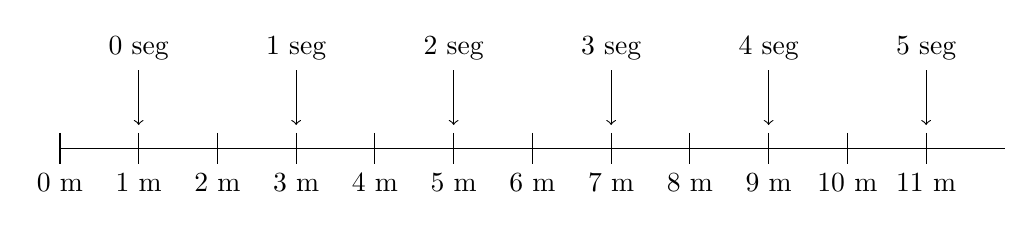
\begin{tikzpicture}
\draw (0,0) -- (12,0);
\foreach \x/\y/\z in {0/1/0,2/3/1,4/5/2,6/7/3,8/9/4,10/11/5}{
  \draw (\x,.2) -- (\x,-.2);
1 \draw (\y,.2) -- (\y,-.2);
  \node [below] at (\x,-.2) {$\x$ m};
  \node [below] at (\y,-.2) {$\y$ m};
  \draw [<-] (\y,.3) -- (\y,1) node [above] {$\z$ seg};
  
}
\end{tikzpicture}
\end{figure}

\item Recomendamos que, se possível, discuta com seus alunos uma variante do problema. O caso em que, mesmo que a pessoa não ande em linha reta, o gráfico continua representando a relação entre a distância percorrida e o tempo de percurso. Apresente por exemplo percursos diferentes, refazendo as perguntas, como por exemplo:

\begin{figure}[H]
\centering
\usetikzlibrary{arrows.meta}


\begin{tikzpicture}[scale=.75]
\draw circle (2cm);
\node at (0:2) {$\times$} node at (0:2) [right, overlay] {Ponto de partida}; 
\node at (300:2) {$\times$} node at (300:2) [below right, overlay] {Ponto de referência}; 

\draw [-{>[length=2mm,width=3mm]},  samples=1000] (2,0) arc (0:30:2);
\draw [-{>[length=2mm,width=3mm]}, samples=1000] (2,0) arc (0:60:2);

\begin{scope}[scale=2,shift={(3.5,.25)}]
\draw (0,0) -- (2,0) -- (.2,-1) -- (-.2,-.2);
\node at (0,0) {$\times$};
\node [above] at (0,0) {Ponto de referência};
\node at (2,0) {$\times$};
\node [right,] at (2,0) {Ponto de partida};
\end{scope}
\end{tikzpicture}

\end{figure}


\item Discuta com seus alunos o motivo da função não ser linear e consequentemente, nesta situação, a relação entre as grandezas não ser proporcional. Utilize o fato de não atender o Teorema Fundamental da Proporcionalidade.

\item Caso seus alunos já tenham estudado esse conteúdo em Física, aproveite para relacionar a função $f(t)=at+b$ com a equação tradicional do Movimento Uniforme: $S=S+Vt$, associando S com $f(t)$ ; $S_0$ com $b$ e $V$ com $a$.
 
\end{itemize}
}{0}{2}
\end{sugestions}
\marginpar{\vspace{.5em}}
\begin{answer}{Distância $\times$ tempo}
{
\begin{enumerate}
\item $1$ metro. $9$ metros.
\item $8$ metros.
\item Sim, ela está se afastando. A medida que o tempo aumenta a distância até o ponto de referência também aumenta. Isto é, a função é crescente.
\item A velocidade média é $V=9−14−0=2$ m/s.
\item $3$ metros. $2$ metros.
\item $3$ metros em ambos os intervalos de tempo.
\item A cada segundo a pessoa se afasta $2$ metros do ponto de referência.
\item Não, pois a distância até o ponto de referência em $2$ segundos é $5$ metros e em $1$ segundo é $3$ metros, ou basta ver que o gráfico não passa pela origem do plano cartesiano .
\end{enumerate}
}{1}
\end{answer}
\explore{Função Afim}
\label{\detokenize{AF107-4:sec-funcao-afim}}\label{\detokenize{AF107-4::doc}}\label{\detokenize{AF107-4:explorando-funcao-afim}}

\begin{task}{distância x tempo}
\label{ativ-dist-tempo}

O gráfico a seguir mostra a variação da distância a um ponto de referência de uma pessoa que caminha em linha reta durante \(4\) segundos. Algumas informações sobre o movimento podem ser extraídas diretamente dessa representação gráfica.
\phantomsection\label{\detokenize{AF107-4:fig-tempo-distancia}}
\begin{figure}[H]
\centering

\begin{tikzpicture}[yscale=.75]

\draw [dashed, help lines, thin] (0,0) grid (4.5,9.5);
\draw [->] (-1,0) -- (4.5,0);
\draw [->] (0,-1) -- (0,9.5);

\draw [\currentcolor, very thick] (0,1) -- (4,9) node [above right] {$f$};
\draw [thick, dashed] (0,1) -- (4.5,1);
\draw [thick, dashed] (4,0) -- (4,9);
\draw [thick, dashed] (0,9) -- (4,9);

\foreach \x in {1,...,4}{
\draw [ thick] (\x,-.1) -- (\x,.1);
\node [below] at (\x,-.1) {\x};}

\foreach \x in {2,4,...,8} \node [left] at (-.1,\x) {\x};
\foreach \x in {1,...,9} \draw [thick] (-.1,\x) -- (.1,\x);

\node [below] at (2,1) {tempo decorrido};
\node [left] at (0,1) {início};
\node [rotate=90, above] at (-.5,8) {distância ($m$)};
\node [rotate=90, below] at (4.5,5) {distância percorrida};
\node [right] at (4.5,0) {tempo ($s$)};
\end{tikzpicture}


\label{\detokenize{AF107-4:fig-tempo-distancia}}\end{figure}
\begin{enumerate}
\item {} 
A que distância do ponto de referência estava a pessoa no início da contagem do tempo? E ao final de \(4\) segundos?

\item {} 
Qual a distância total percorrida?

\item {} 
É possível saber se ele está se afastando ou se aproximando do ponto de referência? Como?

\item {} 
Qual a velocidade média da pessoa no intervalo de tempo de \(0\) a \(4\) segundos?

\item {} 
A que distância a pessoa estava do ponto de referência após \(1\) segundo do início da caminhada? Qual a distância percorrida por ela nesse intervalo de tempo?

\item {} 
Qual a distância percorrida pela pessoa entre \(1\) e \(2\) segundos? E entre \(3\) e \(4\) segundos?

\item {} 
O que se pode concluir, a partir das suas respostas nos itens (e) e (f), sobre a variação da distância percorrida a cada minuto de caminhada?

\item {} 
As grandezas relacionadas pelo gráfico são proporcionais? Porque?

\end{enumerate}

\end{task}

\clearpage
\def\currentcolor{session4}
\begin{sugestions}{}
{
\begin{figure}[H]
\centering

\noindent\includegraphics[width=100bp]{{codigo3_3}.png}
\end{figure}

Sugerimos o uso da construção GeoGebra disponível no endereço \url{https://www.geogebra.org/m/NFAmT23H}. Nela os estudantes poderão experimentar dinamicamente propriedades de crescimento, decrescimento e interseção com os eixos coordenados associadas à função afim \(f(x)=ax+b\), em que \(a\) e \(b\) variam no intervalo \([-5,5]\).
}{1}{2}
\end{sugestions}

\arrange{Função Afim}
\label{\detokenize{AF107-4:organizando-as-ideias-funcao-afim}}
O gráfico da atividade \hyperref[ativ-dist-tempo]{distância x tempo} apresenta a distância até o ponto de referência como uma função do tempo. Como a ação acontece no intervalo de tempo de \(0\) a \(4\) segundos, podemos modelar essa relação com uma função \(f\) cujo domínio é o intervalo \([0,4]\), isto é, \(f:[0,4] \to \mathbb{R}\). Vamos juntos determinar uma expressão para \(f\)?

Apesar do gráfico ser um segmento de reta, \(f\) não pode ser uma função linear, pois a reta não contém a origem do plano cartesiano. Como no início da contagem do tempo a pessoa estava na posição \(1\), devemos ter \(f(0)=1\). Em particular, as grandezas posição e tempo, nesse caso, não são proporcionais.

Vamos considerar, como na atividade, a relação de outra grandeza com o tempo: a distância percorrida do início até o instante $ t $. Nesse caso temos proporcionalidade e vamos ver por quê.

\begin{minipage}{0.6\textwidth}
Para facilitar a discussão, chamemos essa função de $ d(t) $. Seu domínio coincide com o domínio de $ f $ e podemos dizer que \(d(t)\) é a distância percorrida no intervalo de tempo \([0,t]\). Por exemplo, como fazemos para calcular \(d(2)\) ? Basta saber em que posições a pessoa estava nos tempos \(t=0\) e \(t=2\) e fazer a diferença. Neste caso \(d(2)=f(2)-f(0)=5-1=4\). Isso nos dá a dica de como calcular \(d(t)\) para qualquer \(t\in[0,4]\).
\end{minipage}
\begin{minipage}{0.3\textwidth}
\begin{table}[H]
\centering
\begin{tabular}{|l|c|}
\hline
\tcolor{$t$} & \tcolor{$d(t)$} \\ 
\hline 
$0$ & $ 1-1=0 $ \\ 
\hline 
$1$ & $ 3-1=2 $ \\ 
\hline 
$2$ & $ 5-1=4 $ \\ 
\hline 
$3$ & $ 7-1=6 $ \\ 
\hline 
$4$ & $ 9-1=8 $ \\ 
\hline
\end{tabular}
\end{table}
\end{minipage}

\[
d(t)=f(t)-f(0) \Longrightarrow d(t)= f(t)-1.
\]

Por causa dessa última relação, o gráfico de $ d $ será exatamente igual ao gráfico de $ f $, deslocado uma unidade para baixo. Ou seja, uma reta paralela a que é o gráfico de $ f $ e que passa pela origem. Conclusão, $d(t)$ é uma função linear, e, como $ d(1)=2 $, podemos afirmar que $ d(t)=2t $.
\begin{figure}[H]
	\centering
\begin{tikzpicture}[yscale=.75]

\draw [dashed, help lines, thin] (0,0) grid (4.5,9.5);
\draw [->] (-1,0) -- (4.5,0);
\draw [->] (0,-1) -- (0,9.5);

\draw [dashed, very thick] (0,1) -- (4,9) node [above right] {$f$};
\draw [\currentcolor, very thick] (0,0) -- (4,8) [above right] node {$d$};

\fill (2.5,5) circle (2.pt);
\fill (2.5,6) circle (2pt);
\draw [dashed, thick] (2.5,5) -- (2.5,6);

\foreach \x in {1,...,4}{
\draw [ thick] (\x,-.1) -- (\x,.1);
\node [below] at (\x,-.1) {\x};}

\foreach \x in {2,4,...,8} \node [left] at (-.1,\x) {\x};
\foreach \x in {1,...,9} \draw [thick] (-.1,\x) -- (.1,\x);

\node [below] at (2,1) {tempo decorrido};
\node [left] at (0,1) {início};
\node [rotate=90, above] at (-.5,8) {distância ($m$)};
\node [rotate=90, below] at (4.5,5) {distância percorrida};
\node [right] at (4.5,0) {tempo ($s$)};
\end{tikzpicture}
\end{figure}

Pelo que tínhamos visto, $ d(t)=f(t)-1 $, o que nos leva à expressão
\[
f(t)=2t+1
\]

\begin{observation}
Chamamos qualquer função que pode ser escrita dessa forma de uma \textbf{função afim}, isto é, toda função real que pode ser escrita da forma
\[
f(x)=ax+b
\]
para quaisquer números reais $ a\neq 0 $ e $ b$. O gráfico de uma função afim é sempre uma reta, paralela à reta gráfico da função linear $ \ell(x)=ax $ deslocada $b$ unidades na vertical.

O número $ a $ é a \textbf{taxa de variação média} da função afim $ f $ (e da função linear também) em qualquer intervalo.
\[
\dfrac{\Delta f}{\Delta x}= \dfrac{f(x_2)-f(x_1)}{x_2-x_1}= \dfrac{ax_2+b-(ax_1+b)}{x_2-x_1}= \dfrac{a(x_2-x_1)}{x_2-x_1}=a.
\]


\begin{figure}[H]
\centering

\begin{tikzpicture}[scale=.8]

\draw [->] (-2,0) -- (5,0);
\draw [->,thick] (0,-1) -- (0,6);
\draw [|-|, thick] (1,1) -- (1,3.5) node [midway, left] {$b$};
\draw [domain=-1:5, very thick, dashed] plot (\x,{\x}) node [rotate=45, above, shift={(-1.5,0)}] {$\ell(x)=ax$};
\draw [domain= -2:3.5, \currentcolor!80, very thick] plot (\x,{\x+2.5}) node [rotate=45, above, shift={(-1.5,0)}] {$f(x)=ax+b$} ;

\end{tikzpicture}

\end{figure}

\end{observation}

\begin{example}{}

\begin{figure}[H]
\centering
\capstart

\begin{tikzpicture}[scale=.6]

\draw [ thin, step=2, dashed, gray!50] (-4.5,-4.5) grid (8.5,7.5);
\draw [->] (-4.5,0) -- (8.5,0);
\draw [->] (0,-4.5) -- (0,7.5);
\clip (-4.5,-4.5) rectangle (8.5,7.5);

\foreach \x in {-3,...,-1,1,2,...,8} \node [below, scale=.75] at (\x,0) {\x};
\foreach \x in {-4,...,-1,1,2,...,7} \node [left, scale=.75] at (0,\x) {\x};
\node [above left, scale=.75] at (0,0) {0};

\draw [destacado, very thick] plot (\x,{2*\x+5}) node [rotate =63.43494, pos=0.7, shift={(2,2.1)}] {$f(x)=2x +5$};;; 
\draw [very thick, dashed] plot (\x,{2*\x}) node [rotate =63.43494, pos=0.7, shift={(5,0)}, above] {$\ell(x)=2x$};
\draw [domain=-5: 12, \currentcolor, very thick] plot (\x,{2*\x-3}) node [rotate =63.43494, pos=0.7, shift={(5,-1.7)}, above] {$g(x)=2x -3$};;

\end{tikzpicture}

\caption{Exemplos: \(\ell(x)=2x\), \(f(x)=2x+5\) e \(g(x)=2x-3\)}\label{\detokenize{AF107-4:id1}}\end{figure}

\begin{figure}[H]
\centering
\capstart

\begin{tikzpicture}[scale=.7]

\draw [ thin, step=2, dashed, gray!50] (-4.5,-4.5) grid (8.5,7.5);
\draw [->] (-4.5,0) -- (8.5,0);
\draw [->] (0,-4.5) -- (0,7.5);
\clip (-4.5,-4.5) rectangle (8.5,7.5);

\foreach \x in {-3,...,-1,1,2,...,8} \node [below, scale=.75] at (\x,0) {\x};
\foreach \x in {-4,...,-1,1,2,...,7} \node [left, scale=.75] at (0,\x) {\x};
\node [above left,scale=.75] at (0,0) {0};

\draw [destacado, very thick, domain=-2:8.5] plot (\x,{-\x+6}) node [rotate =-45, pos=0.7, shift={(1,3.3)}, above] {$g(x)=-x+6$};

\draw [very thick, dashed] plot (\x,{-\x}) node [rotate =-45, pos=0.7, shift={(-3,0)}, above] {$\ell(x)=-x$};

\draw [domain=-5: 12, \currentcolor, very thick] plot (\x,{-\x-2}) node [rotate =-45, pos=0.7, shift={(0,-2)}, above] {$f(x)=-x-2$};;

\end{tikzpicture}

\caption{Exemplos: \(\ell(x)=-x\), \(f(x)=-x-2\) e \(g(x)=-x+6\)}\label{\detokenize{AF107-4:id2}}\end{figure}
\end{example}

\subsection{A inclinação de uma reta e a taxa de variação média}

\begin{figure}[H]
\centering
\capstart

\noindent\includegraphics[width=250bp]{{1024px-Planalto_Palace_ramp_and_parlatorium}.jpg}
\caption{Flickr: \href{https://commons.wikimedia.org/w/index.php?curid=18864847}{Palácio do Planalto, Brasília, Brasil}}\label{\detokenize{AF107-4:id3}}\end{figure}

Em muitas construções, quando se deseja fazer o acesso entre dois espaços que estão em níveis diferentes, usa-se a rampa como recurso. A rampa é uma superfície, em geral plana, que liga dois níveis diferentes. Uma característica importante de uma rampa é a sua inclinação (ou declive). Rampas muito íngremes podem se tornar obstáculos intransponíveis para cadeirantes, por exemplo. Como medir, então, a inclinação de uma rampa?
A inclinação de uma rampa é o número obtido quando dividimos a altura (diferença entre os níveis) pelo deslocamento horizontal
\begin{figure}[H]
\centering

\noindent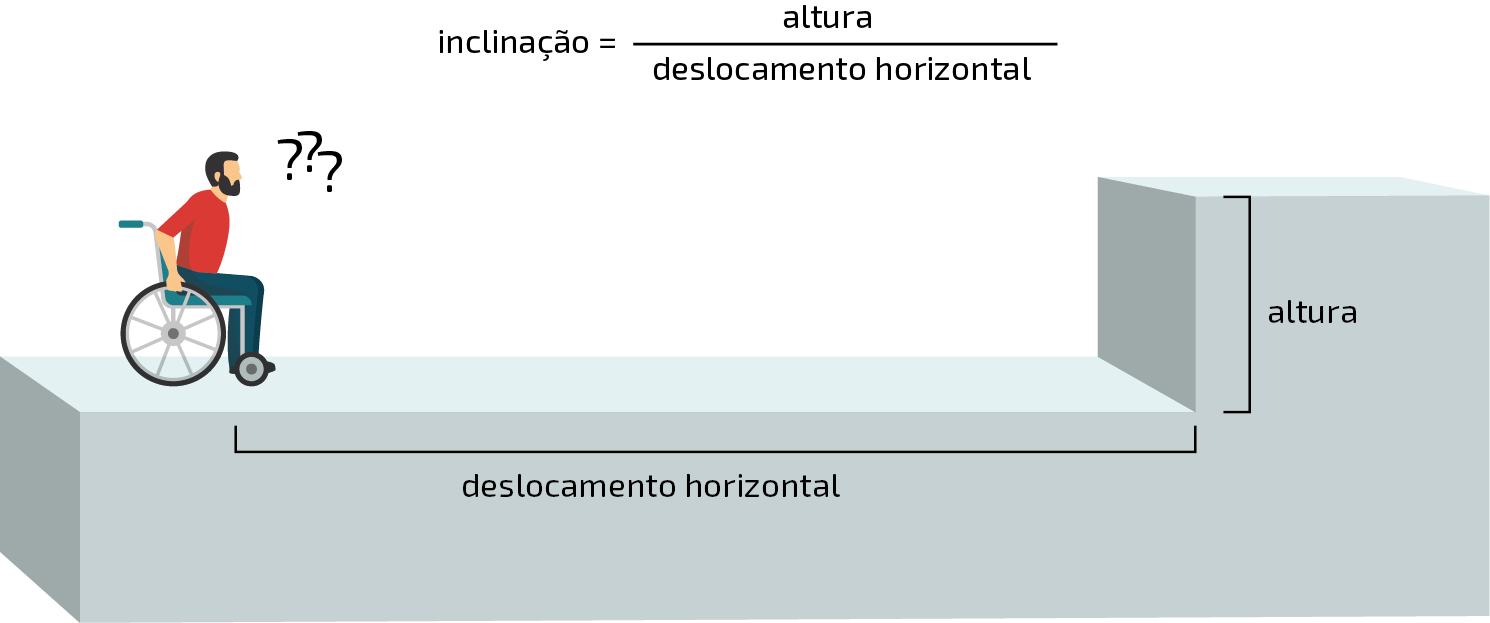
\includegraphics[width=\linewidth]{rampa.png}
\end{figure}
Uma rampa que tem o deslocamento horizontal muito menor que a altura, terá pela fórmula uma inclinação grande, enquanto uma rampa em que o deslocamento horizontal é bem maior que a altura, terá uma inclinação pequena. Rampas de inclinação pequena são as mais desejáveis.

A Associação Brasileira de Normas Técnicas (ABNT) tem normas para a construção de rampas (a NBR 9050:2015 que pode ser acessada \href{http://www.ufpb.br/cia/contents/manuais/abnt-nbr9050-edicao-2015.pdf}{neste link}) que contém o seguinte artigo:


\begin{quote}
6.6.2.1 As rampas devem ter inclinação de acordo com os limites estabelecidos na Tabela. Para inclinação entre $6{,}25\%$ e $8{,}33\%$ é recomendado criar áreas de descanso (6.5.) nos patamares, a cada $50$m de percurso. Excetuam-se deste requisito as rampas citadas em 10.4 (plateia e palcos), 10.12 (piscinas) e 10.14 (praias).
\end{quote}

\begin{table}[H]
\centering
\begin{tabular}{|c|c|c|}
\hline
\tcolor{\parbox[1cm]{3.5cm}{\centering\vspace{.3em} Desníveis máximos de cada segmento de rampa\newline$h$}} & \tcolor{\parbox[1cm]{3.5cm}{\centering\vspace{.3em} Inclinação admissível em cada segmento de rampa $i$}} & \tcolor{\parbox{4cm}{\centering Número máximo de segmentos de rampa}} \\[.25cm]
\hline
$1{,}50$ & $5{,}00 (1:20)$ & Sem limite \\
\hline
$1{,}00$ & $5{,}00 (1:20) < i \leq 6{,}25 (1:16)$ & Sem limite \\
\hline
$0{,}80$ & $6{,}25 (1:16) < i \leq 8{,}33 (1:12)$ & 15\\
\hline
\end{tabular}
\end{table}

Por exemplo, para uma rampa ter inclinação \(5\% (1:20)\) ela precisa de \(20\) metros de deslocamento horizontal para cada metro de subida, ou dito de outra forma, para cada metro de deslocamento horizontal, a rampa “sobe” \(0,05\) metros. Veja se as rampas ilustradas abaixo estão dentro das especificações da ABNT.

Da mesma forma, a inclinação de uma reta é a medida do quão íngreme ela é em relação ao sistema de coordenadas onde ela está inserida. Dada uma reta em um plano cartesiano, para determinarmos sua inclinação basta fazer a divisão entre a variação das ordenadas e a variação das abscissas para quaisquer dois pontos da reta
\begin{equation*}
\begin{split}\text{inclinação}=\dfrac{y_2-y_1}{x_2-x_1}\end{split}
\end{equation*}
\begin{figure}[H]
\centering
\capstart

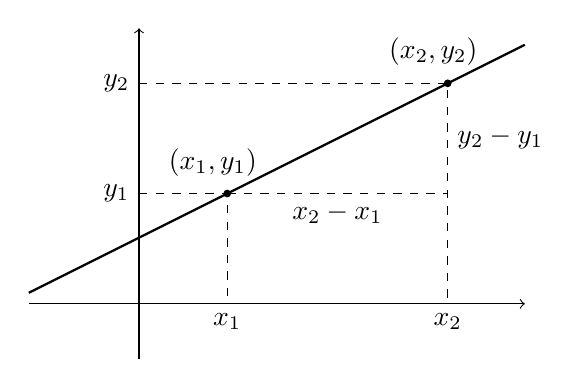
\begin{tikzpicture}[scale=.7, every node/.style={scale=1}]

\draw [->] (-2,0) -- (7,0);
\draw [->] (0,-1) -- (0,5);

\draw [dashed] (0,2) -- (1.6,2) -- (1.6,0);
\draw [dashed] (0,4) -- (5.6,4) -- (5.6,0);
\draw [dashed] (1.6,2) -- (5.6,2);

\draw [domain=-2:7, thick] plot (\x,{.5*\x+1.2});

\fill (1.6,2) circle (2pt);
\fill (5.6,4) circle (2pt);

\node [left] at (0,2) {$y_1$};
\node [left] at (0,4) {$y_2$};

\node [below] at (1.6,0) {$x_1$};
\node [below] at (5.6,0) {$x_2$};

\node [above left, shift={(.5,.1)}] at (1.6,2) {$(x_1,y_1)$};
\node [above left, shift={(.5,.1)}] at (5.6,4) {$(x_2,y_2)$};

\node [right] at (5.6,3) {$y_2-y_1$};
\node [below] at (3.6,2) {$x_2-x_1$};
\end{tikzpicture}
\caption{Inclinação de uma reta}\label{\detokenize{AF107-4:fig-inclina}}\label{\detokenize{AF107-4:id4}}\end{figure}

Por exemplo, a reta que contém os pontos \((1,2)\) e \((5,7)\) tem inclinação \(\dfrac{7-2}{5-1}=\dfrac 54\), enquanto a reta que contém os pontos \((-1,3)\) e \((2,-6)\) tem inclinação \(\dfrac{-6-3}{2-(-1)}=\dfrac{-9}{3}=-3\).

\begin{figure}[H]
\centering
\capstart

\begin{tikzpicture}[scale=.6, every node/.style={scale=1}]

\draw [->] (-2,0) -- (7,0);
\draw [->] (0,-1) -- (0,8);

\draw [dashed] (0,2) -- (1,2) -- (1,0);
\draw [dashed] (0,7) -- (5,7) -- (5,0);
\draw [dashed] (1,2) -- (5,2);

\draw [domain=-1:5.5, thick] plot (\x,{(5/4)*\x+0.75});

\fill (1,2) circle (2pt);
\fill (5,7) circle (2pt);

\node [left] at (0,2) {$2$};
\node [left] at (0,7) {$7$};

\node [below] at (1,0) {$1$};
\node [below] at (5,0) {$5$};

\node [right, scale=1] at (5.5,4.5) {$\displaystyle \frac{7-2}{5-1}=\frac{5}{4}$};
\end{tikzpicture}

\caption{Inclinação da reta que contém os pontos \((1,2)\) e \((5,7)\)}\label{\detokenize{AF107-4:fig-inclina-1}}\label{\detokenize{AF107-4:id5}}\end{figure}

\begin{figure}[H]
\centering
\capstart

\begin{tikzpicture}[scale=.5,remember picture, shift={(1,0)}]

\draw [->] (-2.5,0) -- (3.5,0);
\draw [->] (0,-7.5) -- (0,4.5);

\draw [dashed] (0,3) -- (-1,3) -- (-1,0);
\draw [dashed] (0,-6) -- (2,-6) -- (2,0);
\draw [dashed] (-1,3) -- (2,3) -- (2,0);

\draw [domain=-1.5:2.5, thick] plot (\x,{-3*\x});

\fill (-1,3) circle (2pt);
\fill (2,-6) circle (2pt);

\node [above left] at (0,3) {$3$};
\node [left] at (0,-6) {$-6$};

\node [below] at (-1,0) {$-1$};
\node [below right] at (2,0) {$2$};

\node [right, scale=1] at (2.5,1.5) {$\displaystyle \frac{-6-3}{2-(-1)}=-3$};
\end{tikzpicture}
\caption{Inclinação da reta que contém os pontos \((-1,3)\) e \((2,-6)\)}\label{\detokenize{AF107-4:fig-inclina-2}}\label{\detokenize{AF107-4:id6}}\end{figure}

Se considerarmos uma reta no plano e a função afim \(f\) que a tem como gráfico, a inclinação da reta coincide com a taxa de variação da função \(f\).

Por exemplo, a reta da \hyperref[AF107-4:fig-inclina-1]{Figura \ref{AF107-4:fig-inclina-1}} acima é o gráfico da função afim \(f(x)=\dfrac 54 x +b\). Para determinarmos o valor de \(b\), basta substituirmos um dos pontos que estão sobre a reta. Como \((1,2)\) pertence ao gráfico de \(f\), podemos afirmar que \(f(1)=2\), logo
\begin{equation*}
\begin{split}2=\dfrac 54 \cdot 1 + b \Longrightarrow b=2-\dfrac 54 = \dfrac 34\end{split}
\end{equation*}
Isto é, a função \(f\) é dada pela expressão \(f(x)=\dfrac 54 x + \dfrac 34\).

Já a reta da \hyperref[AF107-4:fig-inclina-2]{Figura \ref{AF107-4:fig-inclina-2}} tem expressão \(f(x)=-3x\).

Retas horizontais não possuem inclinação, de fato não há deslocamento vertical quando nos deslocamos horizontalmente sobre a reta, ou seja, sua inclinação será igual a zero.

\clearpage
\def\currentcolor{session2}
\begin{objectives}{Antecipando o pagamento de uma dívida}
{
\begin{itemize}
\item Relacionar função afim de domínio discreto com progressões aritméticas.
\item Perceber nas sequências apresentadas que a diferença entre termos consecutivos é constante, e portanto elas formam uma P.A.
\end{itemize}
}{1}{2}
\end{objectives}
\begin{sugestions}{Antecipando o pagamento de uma dívida}
{
\begin{itemize}
\item Questione seus estudantes sobre o fato de, apesar da variação ser sempre de \textit{250} reais, em um caso a primeira função (valor a pagar) é decrescente e a segunda função (desconto) é crescente, relacionando com as expressões obtidas no item f).
\item No item d) espera-se que a resposta seja em forma de porcentagem. Caso julgue necessário, aproveite o momento para fazer uma rápida revisão sobre o assunto.
\item Possivelmente os estudantes não estão familizarizados com alguns dos termos apresentados nessa atividade: \textit{\textbf{antecipação de uma dívida, desconto comercial, tempo de antecipação}}. Antes de iniciar a atividade esclareça para eles o significado de cada um desses termos.
\end{itemize}
}{1}{2}
\end{sugestions}
\begin{answer}{Antecipando o pagamento de uma dívida}
{
\begin{enumerate}
\item \adjustbox{valign=t}
{
\begin{tabular}{|l|c|c|c|c|}
\hline
\tcolor{Antecipação (meses)} & \tcolor{5} & \tcolor{6} & \tcolor{7} & \tcolor{8} \\
\hline
Valor a pagar (R\$) & 3.750 & 3.500 & 3.250 & 3.000 \\
\hline
\end{tabular}
}

\item A medida que o tempo aumenta, o valor a pagar diminui. Entre dois meses consecutivos a variação do valor a pagar é de R\$ $250,00$.

\item A medida que o tempo aumenta, o valor do desconto aumenta. Entre dois meses consecutivos a variação do desconto é de R\$ $250,00$.

\item $5\%$ do valor da dívida.

\item \adjustbox{valign=t}
{
\begin{tikzpicture}[xscale=2, scale=.5]
\draw [help lines, ystep=.5] (0,0) grid (9,11);
\draw [-{>[length=2mm,width=3mm]},thick] (0,0) -- (9,0);
\draw [-{>[length=2mm,width=3mm]},thick] (0,0) -- (0,11);
\foreach \x in {1,...,8}
{
\node [below,scale=.75] at (\x,0) {\x};
};
\node [below,left,scale=.75] at (0,0) {0};

\foreach \x/\y in {1/500,2/1000,3/1500,4/2000,5/2500,6/3000,7/3500,8/4000,9/4500,10/5000}
{
\node [left,scale=.75] at (0,\x) {\y};
};

\foreach \x in {0,1,2,3,4,5,6,7,8}{
  \node [fill, circle, inner sep=1pt] at (\x,\x*.5) {};
  \node [fill, circle, inner sep=1pt] at (\x,10-\x*.5) {};
};

\end{tikzpicture}
}

\end{enumerate}
}{2}
\end{answer}
\begin{objectives}{Abastecendo a caixa}
{
\begin{itemize}
\item Identificar a taxa de variação gerada por duas razões distintas.
\item Reconhecer que a taxa de variação é negativa na situação descrita.
\item Relacionar o preenchimento do quadro com a expressão algébrica que modela a situação, sem a necessidade da representação gráfica.
\end{itemize}
}{1}{2}
\end{objectives}
\begin{sugestions}{Abastecendo a caixa}
{
\begin{itemize}
\item Discuta com seus alunos a importância da utilização dos conceitos trabalhados no processo de controle do desperdício de água potável. E como ações simples, pautadas em dados quantitativos podem influenciar na economia de água.
\item Durante a aplicação da atividade, conduza as discussões para que seus alunos argumentem à respeito do sinal da taxa de variação.
\item Possibilite à seus alunos a oportunidade de apresentar soluções diferentes das usuais, seja utilizando conceitos de Progressões aritméticas ou até mesmo de proporcionalidade (fazendo os ajustes necessários, já que $V(0)$ não é zero).
\end{itemize}
}{1}{1}
\end{sugestions}
\begin{answer}{Abastecendo a caixa}
{
\begin{enumerate}
\item $V(t)=−5t+100$.
\item Diminuem.
\item Reduzem $5$ litros em ambos os casos.
\item Em $5$ litros.

\end{enumerate}
}{1}
\end{answer}
\begin{objectives}{Temperatura controlada}
{
\begin{itemize}
\item Obter a expressão algébrica de uma função afim a partir de dois pontos dados no plano cartesiano.
\item Interpretar o ponto de interseção entre as funções que modelam a situação apresentada
\end{itemize}
}{1}{1}
\end{objectives}
\begin{answer}{Temperatura controlada}
{
\begin{enumerate}

\item Como $f$ intersecta o eixo das ordenadas no ponto $A=(0,−4)$ temos que $b=−4$; substituindo o ponto $B=(4,0)$, ou seja, fazendo $f(4)=0$ encontramos $a=1$. Do mesmo modo, $g$ intersecta o eixo das ordenadas no ponto $C=(0,2)$, logo temos que $n=2$; substituindo o ponto $D=(2,0)$, ou seja, fazendo $f(2)=0$ encontramos $m=−1$.

\item Observando os gráficos temos que: a temperatura do composto associado à função $f$ está aumentando, e a temperatura do composto associado à função g está diminuindo.
\begin{enumerate}
\item Fazendo $f(t)=1$ encontramos $t=5$, ou seja o composto associado à função afim $f$, atinge $1$ $^{\circ}$C após $5$ minutos. E fazendo $g(t)=1$ encontramos $t=1$, ou seja o composto associado à função afim $g$, atinge $1$ $^{\circ}$C após $1$ minuto.

\item Fazendo $f(t)=−3$ encontramos $t=1$, ou seja o composto associado à função afim $f$, atinge $−3$ $^{\circ}$C após $1$ minuto. E fazendo $g(t)=−3$ encontramos $t=5$, ou seja o composto associado à função afim $g$, atinge $−3$ $^{\circ}$C após $5$ minutos.

\item Fazendo $f(t)=−8$ encontramos $t=−4$, ou seja o composto associado à função afim $f$, nunca atingirá essa temperatura, já que $f$ é sempre maior ou igual a $−4$ $^{\circ}$C. E fazendo $g(t)=−8$ encontramos $t=10$, ou seja o composto associado à função afim $g$, atinge $−8$ $^{\circ}$C após $10$ minutos.

\item Fazendo $f(t)=10$ encontramos $t=14$, ou seja o composto associado à função afim $f$, atinge $10$ $^{\circ}$C após $14$ minutos. E fazendo $g(t)=10$ encontramos $t=−8$, ou seja o composto associado à função afim $g$, nunca atingirá ess a temperatura, já que $g$ é sempre menor ou igual a $2$ $^{\circ}$C.

\end{enumerate}
\item Basta fazermos $f(t)=g(t)$, ou seja $t−4=−t+2$, resolvendo encontramos $t=3$ minutos, e a temperatura é igual a $f(3)=g(3)=−1$ $^{\circ}$C. Portanto, os dois compostos atigem $−1$ $^{\circ}$C após $3$ minutos de observação.

\end{enumerate}
}{9}
\end{answer}
\clearmargin
\begin{objectives}{Frio nas alturas}
{
\begin{itemize}
\item Explorar o zero da função afim.
\item Compreender em um contexto específico a importância da determinação do zero da função.
\item Perceber que a altitude de acionamento do sistema anti-gelo (o zero da função) se obtém dividindo o valor da temperatura pelo valor absoluto da taxa de variação.
\end{itemize}
}{1}{2}
\end{objectives}
\begin{sugestions}{Frio nas alturas}
{
\begin{itemize}
\item É possível responder à pergunta e) pensando como um problema de progressão aritmética: Se a temperatura local é $30$ $^{\circ}$C e ela diminui $2$ $^{\circ}$C a cada $1.000$ pés, para chegar a zero devemos subtrair $2$ de $30$, um total de $15$ vezes, logo, a altitude é $15.000$ pés.
\item Os itens f) e g) pretendem dar uma ideia de como se obtem a expressão geral do zero da função afim. Caso julgue pertinente, estimule-os a pensar em situações hipotéticas em que as taxas de variação da temperatura em função da altitude sejam diferentem.
\end{itemize}
}{1}{2}
\end{sugestions}
\begin{answer}{Frio nas alturas}
{
\begin{enumerate}

\item $−0{,}002$ $^{\circ}$C/pé
\item $T$ é decrescente, portanto a taxa de variação é negativa.
\item $T(h)=30−0{,}002h$
\item $T(37.200)=−44{,}4$ $^{\circ}$C
\item $15.000$ pés
\item $12.500$ pés
\item Nesse caso, $T(h)=T0−0,{,}02h$. Para determinar a altitude, basta calcular $h$ para o qual se tem $T(h)=0$, isto é, $h=\displaystyle\frac{T_0}{0{,}002}=500T_0$
\end{enumerate}
}{1}
\end{answer}
\clearmargin
\clearmargin
\begin{objectives}{Qual a frequência?}
{
\begin{itemize}
\item Utilizar a ideia de progressão aritmética para resolver um problema.
\end{itemize}
}{1}{2}
\end{objectives}
\begin{sugestions}{Qual a frequência?}
{
\begin{itemize}
\item Evite usar a fórmula $a_n=a_1+(n−1)r$ como único recurso para resolver problemas de P.A. Ela, apesar de parecer prática, pode esconder as ideias simples dos problemas de progressão aritmética. Por exemplo, da 1ª para 70ª frequencia, somamos $69$ vezes a razão. E depois da 70ª para a 86ª, somamos 16 vezes a razão. Isso é mais simples do que escrever $a_70=a_1+(70−1)r$ e $a_86=a_1+(86−1)r$.
\end{itemize}
}{1}{2}
\end{sugestions}
\begin{answer}{Qual a frequência?}
{
\begin{enumerate}

\item 101,7 a 104,9.
\item 101 emissoras FM.
\item Resposta individual.

\end{enumerate}
}{1}
\end{answer}

\practice{Função Afim}
\label{\detokenize{AF107-6::doc}}\label{\detokenize{AF107-6:praticando}}

\begin{task}{Antecipando o pagamento de uma dívida}
\label{\detokenize{AF107-6:atividade-antecipando-o-pagamento-de-uma-divida}}\label{\detokenize{AF107-6:ativ-titulo-da-atividade}}


O cliente de um banco foi à sua agência de relacionamento para negociar a antecipação de uma dívida no valor de R\$ \( 5.000,00\), que venceria no prazo de 8 meses. Lá, foi informado pelo gerente que a modalidade praticada era a de desconto comercial, no qual o valor a ser descontado é calculado a partir do valor da dívida e é proporcional ao tempo de antecipação. Para o caso em questão, o gerente gerou a seguinte quadro:

\begin{table}[H]
\centering
\begin{tabular}{|l|c|c|c|c|c|}
\hline
\tcolor{Antecipação (meses)} & \tcolor{0} & \tcolor{1} & \tcolor{2} & \tcolor{3} & \tcolor{4} \\
\hline
Valor a pagar (R\$) & 5.000 & 4.750 & 4.500 & 4.250 & 4.000 \\
\hline
\end{tabular}
\end{table}

\begin{enumerate}
\item {} 
Observando o padrão de desconto, complete a tabela até o 8º mês de antecipação.

\item {} 
Descreva a variação sofrida pelo valor a pagar à medida que aumenta o tempo de antecipação. O que se pode afirmar sobre a variação observada no valor a pagar entre dois meses consecutivos?

\item {} 
Descreva a variação sofrida pelo valor do desconto à medida que aumenta o tempo de antecipação. O que se pode afirmar sobre a variação observada no valor de desconto entre dois meses consecutivos?

\item {} 
Qual é, então, a taxa mensal de desconto comercial praticada pelo banco?

\item {} 
No plano cartesiano a seguir estão representados os pares ordenados \((n,D(n))\) em que \(n\) é o tempo de antecipação e \(D(n)\) o valor do desconto correspondente. Represente nele os pontos que correspondem aos pares ordenados \((n,V(n))\) em que \(V(n)\) é o valor a pagar no tempo \(n\).

\end{enumerate}
\end{task}


\begin{task}{Abastecendo a caixa}
\label{\detokenize{AF107-6:atividade-abastecendo-a-caixa}}\label{\detokenize{AF107-6:id1}}

Uma caixa de água é abastecida por uma torneira cujo fluxo de água é constante e igual a \(10\) litros por minuto e, simultaneamente, seu conteúdo escoa, por um ralo, cujo fluxo de água é controlado à razão constante de \(15\) litros por minuto. Em certo instante, o volume de água dentro da caixa é de \(100\) litros, estando a torneira e o ralo ambos abertos.
\begin{enumerate}
\item {} 
Sendo $V(t)$ o volume de água na caixa após t minutos do instante citado. Exiba uma sentença matemática para $V(t)$.

\item {} 
Complete a tabela abaixo com os valores correspondentes ao volume de água na caixa.

\begin{table}[H]
\centering
\begin{tabular}{|l|c|c|c|c|c|c|c|c|}
\hline
\tcolor{Tempo (minutos)} & \tcolor{0} & \tcolor{1} & \tcolor{2} & \tcolor{3} & \tcolor{4} & \tcolor{5} & \tcolor{10} & \tcolor{20} \\
\hline
Volume (litros) & & 4 & & & & & & \\
\hline
\end{tabular}
\end{table}

\item {} 
À medida que os valores do tempo aumentam, o que ocorre com os valores correspondentes ao volume de água da caixa?

\item {} 
Quando os valores do tempo aumentam de \(t=1\) a \(t=2\), o quanto variam os valores correspondentes ao volume de água da caixa? E quando estes valores aumentam de \(t=12\) a \(t=13\)?

\item {} 
Quando os valores do tempo aumentam em uma unidade, a partir de um instante qualquer, o quanto variam os valores correspondentes ao volume de água da caixa?

\end{enumerate}
\end{task}


\begin{task}{Temperatura Controlada}
\label{\detokenize{AF107-6:atividade-temperatura-controlada}}\label{\detokenize{AF107-6:id2}}
Num laboratório, um químico conseguiu controlar a variação de temperatura de dois compostos. A variação de ambos está associada às funções afins \(f\) e \(g\), de maneira que a taxa de variação das temperaturas de cada um dos compostos seja constante. Observe o gráfico, onde o eixo das ordenadas indica a temperatura (em graus Celsius) de cada composto em função do tempo \(t\), em minutos. O gráfico da figura a seguir modela a situação:

O gráfico da função \(f\) passa pelos pontos \(A=(0,-4)\) e \(B=(4,0)\), indicando que o composto associado à \(f\) está com uma temperatura de \(-4\,^{\circ}\mathrm{C}\) no início da medição e após \(4\) minutos a temperatura atinge \(0\,^{\circ}\mathrm{C}\).

O gráfico da função \(g\) passa pelos pontos \(C=(0,2)\) e \(D=(2,0)\), indicando que o composto associado à \(g\) está com uma temperatura de \(2\,^{\circ}\mathrm{C}\) no início da medição e após \(2\) minutos a temperatura atinge \(0\,^{\circ}\mathrm{C}\).

Com base nas informações do texto responda as perguntas a seguir:
\begin{enumerate}
\item {} 
Determine as expressões das funções afins \(f\) e \(g\).

\item {} 
A temperatura do composto associado à função \(f\) estão aumentando ou diminuindo? E do composto associado à função \(g\)?

\item {} 
Em quanto tempo cada composto atinge a temperatura de

\begin{enumerate}
\item \(1\,^{\circ}\mathrm{C}\)?

\item \(-3\,^{\circ}\mathrm{C}\)?

\item \(-8\,^{\circ}\mathrm{C}\)?

\item \(10\,^{\circ}\mathrm{C}\)?
\end{enumerate}
\item {} 
Após quantos minutos os dois compostos terão a mesma temperatura? E que temperatura é essa?

\end{enumerate}
\end{task}


\begin{task}{Frio nas alturas}
\label{\detokenize{AF107-6:atividade-frio-nas-alturas}}\label{\detokenize{AF107-6:id3}}

Mesmo em pleno verão um avião, precisa lidar com temperaturas muito baixas. Quando uma aeronave opera em baixas temperaturas, com umidade presente, há a possibilidade de formação de gelo que virá a se acumular na sua estrutura ou em seu grupo moto-propulsor. O gelo se forma quando um avião voa através de uma nuvem ou de um ambiente contendo gotículas de água super-resfriadas. O principal problema causado pela formação de gelo é a modificação do fluxo de ar sobre as superfícies das asas, prejudicando assim o desempenho da nave e acarretando, eventualmente, em mais gastos de combustível. Para evitar problemas como esses as aeronaves contam com um sistema anti-gelo que diminui a formação de camadas de gelo em sua fuselagem, produzindo os chamados “rastros de condensação” como na imagem.

\begin{figure}[H]
\centering

\noindent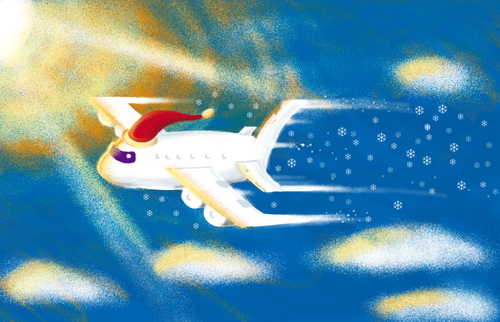
\includegraphics[width=300bp]{frio-aviao.png}
\end{figure}

A temperatura na troposfera (primeira camada da atmosfera que tem aproximadamente \(40.000\) pés de altitude) diminui \(2^\circ\)C a cada aumento de \(1.000\) pés na altitude. Suponha que, em um determinado dia, a temperatura em um aeroporto seja de \(30^\circ\)C, e que a água congela a \(0^\circ\)C.
\begin{enumerate}
\item {} 
Qual a taxa de variação, em \(^\circ C/\text{pé}\), da temperatura da atmosfera, \(T\), em função da altitude, \(h\).

\item {} 
A função \(T(h)\) é crescente ou decrescente? Como isso se reflete na taxa de variação?

\item {} 
Determine uma expressão para \(T(h)\) e represente seu gráfico.

\item {} 
Qual a temperatura a \(37.200\) pés de altitude?

\item {} 
A partir de que altitude o piloto deverá acionar o sistema anti-gelo da aeronave?

\item {} 
Em outro dia, a temperatura no mesmo aeroporto era de \(25^\circ\)C. Qual a altitude de acionamento do sistema anti-gelo, nesse caso?

\item {} 
Estabeleça uma maneira de calcular a altitude de acionamento do sistema anti-gelo quando a temperatura do aeroporto é igual a \(T_0\).

\end{enumerate}
\end{task}

\begin{observation}

Seja \(f:\mathbb{R}\to\mathbb{R}\) uma função afim, \(f(x)=ax+b\), cuja taxa de variação não é nula (isto é, o gráfico de \(f\) não é uma reta horizontal).

A reta que é o gráfico de \(f\), certamente terá interseção com o eixo das abscissas. O valor de \(x\) onde ocorre essa interseção é o zero da função afim.

Seu valor pode ser calculado de duas formas:
\begin{itemize}
\item {} 
Diretamente pela expressão de \(f\):

\end{itemize}
\begin{equation*}
\begin{split}f(k)=0 \Longleftrightarrow ak+b=0 \Longleftrightarrow ak=-b \Longleftrightarrow k=-\dfrac ba\end{split}
\end{equation*}\begin{itemize}
\item {} 
Pelo gráfico, usando semelhança de triângulos:

\end{itemize}

\begin{figure}[H]
\centering

\begin{tikzpicture}
\filldraw [pattern color=\currentcolor!80, pattern=north west lines] (-1.5,0) -- (0,0) -- (0,3);
\filldraw [pattern color=\currentcolor!80, pattern=north west lines] (0,3) -- (1,3) -- (1,5) -- cycle;
\draw [->] (-3,0) -- (3,0);
\draw [->] (0,-2) -- (0,6);

\draw [domain=-2.5:1.3, thick] plot (\x,{2*\x+3});
\fill (0,3) circle (2pt) node [above left] {$(0,b)$};
\fill (-1.5,0) circle (2pt) node [above left] {$(k,0$)};

\node [below] at (-0.75,0) {$-k$};
\node [right] at (0,1.5) {$b$};
\node [below] at (0.5,3) {1};
\node [right] at (1,4) {$a$};

\node [left] at (-.5,5) {$\displaystyle \frac{-k}{1}=\frac{b}{a}\Longrightarrow k=\frac{-b}{a}$};
\end{tikzpicture}
\end{figure}

Por exemplo, o zero da função \(f(x)=5x-21\) é o valor \(k=\dfrac{-(-21)}5\).

Já o zero da função \(g(x)=7-\dfrac x2\) é \(k=\dfrac{-7}{-\frac 12}=14\) .
\end{observation}

\clearpage
\begin{task}{Qual a frequência?}
\label{\detokenize{AF107-6:atividade-qual-a-frequencia}}\label{\detokenize{AF107-6:id4}}

A Agência Nacional de Telecomunicações (ANATEL) determina que as emissoras de rádio FM utilizem as frequências de 87,9 a 107,9MHz, e que haja uma diferença de 0,2MHz entre emissoras com frequências vizinhas.
\begin{enumerate}
\item {} 
Em uma determinada região as frequências entre a 70ª e 86ª são reservadas rádios comunitárias. Determine a frequência mínima e máxima para uma rádio comunitária.

\item {} 
Determine quantas emissoras FM podem funcionar em uma mesma região.

\item {} 
Lembre-se da frequência da rádio que você costuma ouvir e determine a posição dela na sequência das frequências do problema.

\end{enumerate}
\end{task}
\clearpage
\def\currentcolor{session1}
\begin{objectives}{Quadros na parede}
{
\begin{itemize}
\item Introduzir o conceito de Progressão Aritmética.
\item  Fazer medições e criar estratégias para resolver um problema prático.
\item  Obter uma expressão que relacione a distância do gancho até a lateral da parede com o número do gancho.

\end{itemize}
}{1}{1}
\end{objectives}
\begin{sugestions}{Quadros na parede}
{
\begin{itemize}
\item Compartilhe com a turma algumas das soluções encontradas. Estimule que os estudantes descrevam suas estratégias e critiquem o raciocínio uns dos outros.
\item  Considere escrever um resumo dos valores bem-sucedidos no quadro, em
forma de lista.
\item  Não é exigido que os quadros sejam distribuídos de modo que as distâncias do primeiro e último quadros até as paredes laterais sejam iguais. Ou seja, os ganchos podem ser dispostos de modo que o conjunto de quadros fique mais próximo da parede da esquerda ou da direita.
\end{itemize}
}{1}{1}
\end{sugestions}
\begin{answer}{Quadros na parede}
{
\begin{enumerate}
\item Resposta individual;
\item Resposta individual;
\end{enumerate}
}{1}
\end{answer}
\clearmargin
\begin{answer}{Quadros na parede}
{
\begin{enumerate}\setcounter{enumi}{2}
\item Os valores que estão faltando são, nesta ordem, $7$, $15$ e $19$.
\item Uma possibilidade é desenvolver a sequência até o décimo termo que é $43$. Outra possibilidade é utilizar uma expressão que relacione a distância com o número n que indica a posição do quadro na parede, como por exemplo $d(n)=7+4(n-1)$.
\item $d(n)=7+4(n-1).$
\item $d(1)=5m$, $d(6)=15m$, $d(13)$ representa a distância do gancho $13$ até a parede.
\item Ambas se expressaram corretamente, uma vez que as expressões são equivalentes, isto é, $d(n)=10+3(n-1)=7+3n$.  
\end{enumerate}
}{1}
\end{answer}

\explore{Domínios Discretos}

\begin{task}{quadros na parede}
Caso tenha disponibilidade, sugerimos o uso da versão digital desta atividade disponível neste \href{https://teacher.desmos.com/activitybuilder/custom/5e7ba1a876309d7f9879af12}{link}
\begin{figure}[H]
\centering

\includegraphics[width=75bp]{qr_code_quadros}

\end{figure}
Você deseja pedurar três quadros que têm as mesmas dimensões na parede acima do seu sofá. A linha tracejada da figura indica a altura que você deve pedurar os ganhchos. Sem auxílio de instrumentos de medição marque as posições aproximadas dos ganchos sobre a linha tracejada de maneira que os quadros fiquem igualmente espaçados entre si.

\begin{figure}[H]
\centering
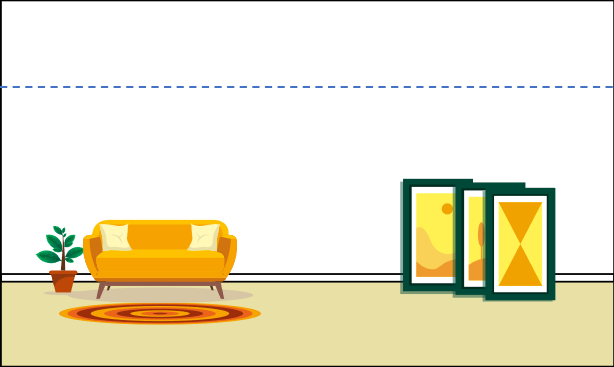
\includegraphics[width=250bp]{quadros_na_parede1}

\caption{Fonte: \href{freepik.com}{Freepik}}

\end{figure}

\begin{enumerate}
\item Marcar as posições "de olho"{}pode gerar imprecisões. Para que fique perfeito é necessário medir e distribuir uniformemente os ganchos. Com o auxílio de uma régua meça a parece acima ($1$cm=$1$m) e marque as posições para os três ganchos de pendurar quadros, precisamente. Use uma caneta de outra cor para comparar com as posições anteriores. Explique sua estratégia.

\item Agora, suponha que você tem uma outra parede representada abaixo em que deseja pendurar cinco quadros equidistantes. Onde você deve posicionar os ganchos? Use o desenho abaixo para indicar e explique a sua estratégia.

\begin{figure}[H]
\centering
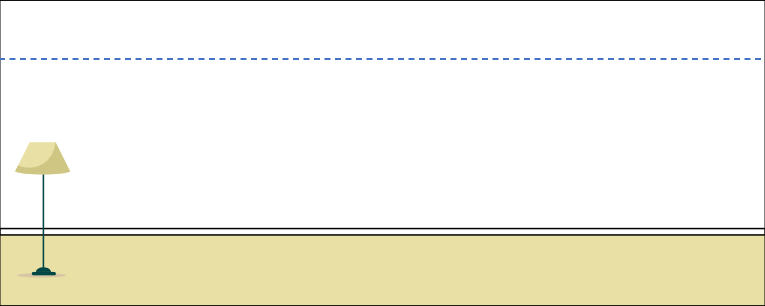
\includegraphics[width=250bp]{quadros_na_parede2}


\end{figure}

\item A tabela a seguir indica duas das distâncias (até o lado esquerdo da parede) de ganchos equidistantes em uma parede. Complete os espaços em branco e explique sua estratégia.

\begin{table}[H]
\centering
\begin{tabular}{|c|c|}
\hline
\tcolor{Gancho} & \tcolor{Distância (m)} \\
\hline
1 & \\
\hline
2 & 11 \\
\hline
3 & \\
\hline
4 & \\
\hline
5 & 23 \\
\hline
\end{tabular}
\end{table}

\item Supona agora que você queira posicionar mais 15 quadros na parede do item anterior, respeitando as distâncias estabelecidas. Como saber a distância, até o lado esquerdo da parede, que se encontra o gancho de número 10? Descreva pelo menos duas estratégias diferentes.

\item Para a parede do item anterior, escreva uma expressão que forneça a distância $d$ dos ganchos até o lado esquerdo da parede em função do número $n$ do gancho.

\item Em uma outra parede a distância dos ganchos \textit{em metros} em função da sua posição é dada por $d(n)=3+2n$. A que distância está o primeiro gancho? E o sexto gancho? O que representa o número $d(13)$?

\item Júlia e Camila usaram as seguintes expressões para representar a tabela a seguir:

\begin{table}[H]
\centering
\begin{tabular}{l>{$}l<{$}}
\text{Júlia} & d(n)=7+3n \\
\text{Camila} & d(n)=10+3(n-1)
\end{tabular}
\end{table}

\begin{table}[H]
\centering
\begin{tabular}{|c|c|}
\hline
\tcolor{Gancho} & \tcolor{Distância (m)} \\
\hline
1 & 10 \\
\hline
2 & 13 \\
\hline
3 & 16 \\
\hline
4 & 19 \\
\hline
5 & 22 \\
\hline
6 & 25 \\ 
\hline
\end{tabular}
\end{table}

Quem das duas se expressou corretamente? Por quê? Como cada uma delas pode ter pensado para chegar nas expressões?

\end{enumerate}

\end{task}

\arrange{Domínios Discretos}

Neste capítulo estamos trabalhando com funções afins e, como você deve ter percebido, na atividade anterior a relação entre as variáveis disância e posição do gancho na fila também estavam relacionadas por uma função afim. O que queremos destacar nesta seção é uma outra maneira de representar a \textbf{função afim} quando seu domínio é um \textbf{conjunto discreto} - em que é possível contar ou enumerar seus elementos, dizer quem é o primeiro, o segundo, o terceiro e assim por diante. Em muitos casos e atividades anteriores, de fato, nos ativemos apenas a um conjunto finito de elementos do domínio, e para esses casos é possível traduzi-los para essa nova notação.

No caso de funções definidas em cojuntos discretos, é possível adotar como domínio padrão o conjunto (ou um subonjunto) dos números naturais $\mathbb{N}=\{1,2,3,4,...\}$. Dessa forma, podemos apenas representar o conjunto imagem como uma sucessão ou sequência de valores ordenados: 
\begin{equation*}
(a_1, a_2,a_3,a_4,...)
\end{equation*}
em que, necessariamente, o termo de índice $n$ está na $n$-ésima posição da lista.

Quando a função em questão é \textit{afim}, chamamos a sequência de valores da imagem de \textbf{progressão aritmética} ou simplesmente uma \textbf{P.A.}. Assim, em uma progressão aritmética, o número que está na $n$-ésima posição da lista pode ser expresso como uma função afim da variável $n$.
\begin{equation*}
a_n=f(n)=\alpha\cdot n+\beta
\end{equation*}
em que $\alpha$ e $\beta$ representam números reais e $\alpha\neq0$

Na atividade anterior, conforme o número de quadros foi amentando, vimos que foi necessário desenvolver uma estratégia para que eles pudessem ser distribuídos de modo que ficassem igualmente espaçados na parede. Se retornarmos ao item \textbf{\textcolor{session1}{c})} e escrevermos lado a lado os valores presentes na segunda coluna da tabela obtemos a sequência (7,11,15,19,23).

Na sequência $(7,11,15,19,23)$ percebemos que a expressão
\begin{equation*}
a_n=4n+3,
\end{equation*}
para $n=1,2,3,4,5$ fornece cada um dos termos da sequência.

A exemplo que foi observado na atividade dos quadros, a diferença entre dois termos consecutivos em uma progressão aritmética é sempre a mesma. Na sequência de vinte termos $(7,11,15,...,83)$ a diferença entre termos consecutivos é igual a 4. Dito de outra forma, cada número é obtido somando 4 ao anterior.
\begin{equation*}
7\xrightarrow{+4} 11 \xrightarrow{+4} 15 \xrightarrow{+4} 19 \xrightarrow{+4} 23 \xrightarrow{+4} \cdots \xrightarrow{+4} 83
\end{equation*}

Esse valor constante que somamos para obter o próximo termo da progressão é chamado de \textbf{razão} da P.A. e coincide com a taxa de variação da função afim que a define.

\begin{equation*}
a_{k+1}=a_k=\alpha(k+1)+\beta-(\alpha+\beta)=\alpha
\end{equation*}
\begin{equation*}
a_1 \xrightarrow{+\alpha} a_2 \xrightarrow{+\alpha} a_3 \xrightarrow{+\alpha} a_4 \xrightarrow{+\alpha}\cdots   
\end{equation*}

\begin{align*}
a_2=&a_1+\alpha\\
a_3=&a_2+\alpha=a_1+2\alpha\\
a_4=&a_3+\alpha=a_2+2\alpha=a_1+3\alpha\\
&\vdots\\
a_n=&a_{n-1}+\alpha=\cdots=a_1+(n-1)\alpha
\end{align*}

Observe então que, para determinar todos os termos de uma progressão aritmética, basta conhecer
\begin{enumerate}
\item dois termos e suas posições, ou
\item um termo em posição e a razão.
\end{enumerate}
Veja os exemplos:

\begin{example}{}
Determinar os elementos de uma P.A. de 10 termos sabendo que $a_2=0{,}9$ e que $a_7=1{,}9$.

\textit{Solução}: Neste caso, para ir do segundo para o sétimo termo, temos que somar 5 vezes a razção. Assim,
\begin{equation*}
1{,}9=0{,}9+5\alpha\Rightarrow\alpha=0{,}2
\end{equation*}

A progressão é $(0{,}7;0{,}9;1{,}1;1{,}3;1{,}5;1{,}7;1{,}9;2{,}1;2{,}3;2{,}5)$
\end{example}
\begin{example}{}
Qual é o trigésimo quarto termo de uma progressão aritmética de razão $\displaystyle\frac{-\pi}{2}$ e cujo termo de posição $12$ é igual a $0$?

\textit{Solução}: Do $a_12$ até o $a_34$ somamos $22$ vezes a razão. Logo,
\begin{equation*}
a_{34}=a_12+22\cdot(\frac{-\pi}{2})=0+22\cdot(\frac{-\pi}{2})=-11\pi.
\end{equation*}
\end{example}

\begin{observation}
De maneira análoga à função afim, se uma progressão aritmética tem razão positiva ela será \textbf{crescente}, e se a razão for um número negativo, ela será \textbf{decrescente}.
\end{observation}

\clearpage
\def\currentcolor{session2}
\begin{objectives}{Termo geral de uma P.A.}
{
\begin{itemize}
\item Objetivos específicos
\item Introduzir a nomenclatura “termo geral” para uma P.A.
\item Identificar os elementos principais dessa fórmula: $a_n, a_1,r$
\end{itemize}
}{1}{1}
\end{objectives}
\begin{sugestions}{Termo geral de uma P.A.}
{
\begin{itemize}
\item Evite estimular a memorização dessa fórmula. Procure explorar o significado da relação entre $a_n$ e $a_1$.
\item As expressões do termo geral podem ficar em função de $n$ ou de $n-1$.
\item Considere extrapolar a fórmula para a relação com outros termos diferentes do primeiro:
\begin{equation*}
a_n=a_k+(n-k)r.
\end{equation*}

\end{itemize}
}{1}{1}
\end{sugestions}
\begin{answer}{Termo geral de uma P.A.}
{
\begin{table}[H]
\centering
\begin{tabular}{|>{$\displaystyle}c<{$}|>{\centering $}m{2cm}<{$}|>{$}c<{$}|>{$\displaystyle}l<{$}|}
\hline
$\tcolor{P.A.}$ & 
$\tcolor{\makecell{Primeiro\\termo}}$ & 
$\tcolor{Razão}$ & 
$\tcolor{\centering Termo Geral}$ \tabularnewline
\hline
(a_1,a_2,a_3) & a_1 & r & a_n=1+2(n-1)=2n-1 \\
\hline
(1,3,5,7,9,...) & 1 & 2 & a_n=1+2(n-1)=2n-1 \\
\hline
(2,4,6,8,10,...) & 2 & 2 & a_n=2+2(n-1)=2n \\
\hline
(3,2,1,0,-1,...)& 3 & -1 & a_n=3-(n-1)=4-n\\
\hline
\Bigg(\frac{49}{5},\frac{48}{5},\frac{47}{5},\frac{46}{5},\frac{45}{5},...\Bigg) & \dfrac{49}{5} & \dfrac{-1}{5} & a_n=10-\dfrac{n}{5} \\
\hline
\Big(\pi,\frac{5\pi}{4},\frac{9\pi}{4},...\Big) & \pi & \frac{\pi}{4} &a_n=\pi+\frac{\pi}{4}(n-1)=\frac{3\pi}{4}+\frac{\pi}{r}n \\
\hline
(4,6,8,10,12,...)& 4 & 2 & a_n=2+2n \\
\hline
\end{tabular}
\end{table}
}{0}
\end{answer}

\begin{objectives}{Quantos múltiplos?}
{
\begin{itemize}
\item Utilizar a mesma estratégia da atividade “Quadros na parede” em um contexto matemático abstrato.
\end{itemize}
}{1}{1}
\end{objectives}
\begin{sugestions}{Quantos múltiplos?}
{
\begin{itemize}
\item Estimule que os estudantes descrevam suas estratégias e critiquem o raciocínio uns dos outros.
\item Caso alguém comece enumerando os múltiplos, peça que tente desenvolver uma estratégia diferente.

\end{itemize}
}{1}{1}
\end{sugestions}
\begin{answer}{Quantos múltiplos?}
{
\begin{enumerate}
\item O primeiro e o último múltiplos de $13$ dentro do intervalo dado são $104$ e $195$, portanto a relação$ 195=104+13(n-1)$, fornece $n=8$.
\item O primeiro e o último múltiplos de $7$ dentro do intervalo dado são $1001$ e $1995$, portanto a relação $1995=1001+7(n-1)$, fornece $n=143$.
\end{enumerate}
}{0}
\end{answer}
\begin{objectives}{Plantas companheiras}
{
\begin{enumerate}
\item Identificar a expressão algébrica que expressa a regularidade observada na sequência apresentada na figura.
\item Identificar funções de domínio discreto e observar a implicação na representação gráfica.
\end{enumerate}
}{1}{2}
\end{objectives}
\marginpar{\vspace{-2em}}
\begin{sugestions}{Plantas companheiras}
{
\begin{itemize}
\item Nesta atividade o estudante deve identificar que o domínio de ambas as funções é um conjunto discreto e que esse fato tem implicações no gráfico das funções, que serão conjuntos de pontos colineares, mas não serão retas.
\item Ainda neste ano de escolaridade boa parte dos alunos terão dificuldades de identificar a expressão algébrica que expressa a relação entre as grandezas apresentadas na figura, caso essa dificuldade atrapalhe o andamento da atividade, sugerimos que o professor intervenha exibindo exemplos mais simples do mesmo assunto.
\item Aproveite para comentar com os alunos que as funções $C(n)$ descrita no item e) é uma função quadrática com domínio discreto, e que esse será o assunto de um capítulo envolvendo funções quadráticas.
\item A atividade aborda assuntos relacionados a dois temas transversais, tais como Meio Ambiente, Saúde e sustentabilidade. Sugerimos que procure fazer um trabalho colaborativo com os professores de Biologia e de Geografia para ampliar a discussão com os alunos sobre os benefícios de uma alimentação orgânica e sobre as questões de viabilidade econômica e de sustentabilidade de tal tipo de cultura. 

\end{itemize}
}{1}{2}
\end{sugestions}
\begin{answer}{Plantas companheiras}
{
  \begin{enumerate}
\item \adjustbox{valign=t}
{
\begin{tabular}{|l|>{\centering}m{2cm}|>{\centering}m{2cm}|}
\hline
\tcolor{} & \tcolor{({\Large$\bullet$})} & \tcolor{({\Large$\diamondsuit$})} \tabularnewline
\hline
Modelo 1 & 1 & 4 \tabularnewline
\hline
Modelo 2 & 4 & 8 \tabularnewline
\hline
Modelo 3 & 9 & 12 \tabularnewline
\hline
Modelo 4 & 16 & 16 \tabularnewline
\hline
\end{tabular}
}

\item A quantidade de vegetais ({\Large$\bullet$}) é o quadrado do número $n$ que identifica a ordem do modelo na sequência

\item A quantidade de plantas companheiras ({\Large$\diamondsuit$}) é o quádruplo do número do modelo.


  \end{enumerate}
}{1}
\end{answer}
\begin{answer}{Plantas companheiras}
{
\begin{enumerate}\setcounter{enumi}{3}
\item $V(n)=n^2$

\item $C(n)=4n$
\clearpage
\item \adjustbox{valign=t}
{
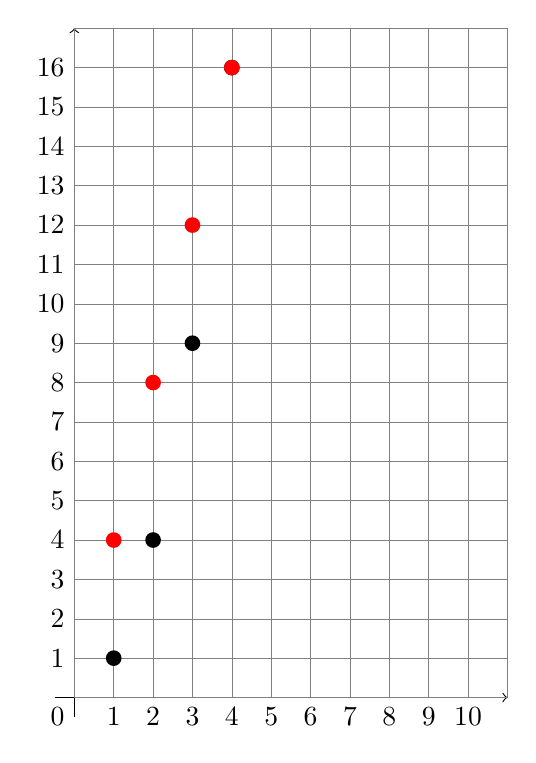
\begin{tikzpicture}[scale=.5]
\draw [->] (-.5,0) -- (11,0);
\draw [->] (0,-.5) -- (0,17);
\draw [help lines] (0,0) grid (11,17);

\foreach \x in {1,...,10} \node [below] at (\x,0) {\x};
\foreach \x in {1,...,16} \node [left] at (0,\x) {\x};
\node [below left] {0};

\foreach \x/\y in {1/1, 2/4, 3/9, 4/16} \node [fill, circle, inner sep=2pt] at (\x,\y) {};

\foreach \x/\y in {1/4, 2/8, 3/12, 4/16} \node [fill, circle, inner sep=2pt, red] at (\x,\y) {};

\end{tikzpicture}
}

\item $C(10)=40$

\item 36
\end{enumerate}
}{1}
\end{answer}
\begin{objectives}{Imagem da P.A.}
{
\begin{itemize}
\item Deduzir que as funções afins preservam progressões aritméticas.
\item Reconhecer a relação entre as razões das P.A. e a taxa de variação das funções afins.
\end{itemize}
}{1}{1}
\end{objectives}
\marginpar{\vspace{-2em}}
\begin{sugestions}{Imagem da P.A.}
{
\begin{itemize}
\item Verifique se as conjecturas do item (e) estão formuladas de maneira precisa, mesmo que sejam textuais.
\item Como a demonstração desse fato é simples, conduza os estudantes para a justificativa/demonstração.
\end{itemize}
}{1}{1}
\end{sugestions}
\begin{answer}{Imagem da P.A.}
{
\begin{enumerate}
\item \adjustbox{valign=t}
{
\begin{tabular}{|>{$}c<{$}|*{9}{c|}}
\hline
\cellcolor{\currentcolor!80}\textcolor{white}{\bm{x}} & 2 & 5 & 8 & 11 & 14 & 17 & 20 & 23 & 26 \\
\hline
\cellcolor{\currentcolor!80}\textcolor{white}{\bm{f(x)}} & 7 & 16 & 25 & 34 & 43 & 52 & 61 & 70 & 79 \\
\hline
\cellcolor{\currentcolor!80}\textcolor{white}{\bm{g(x)}} & -8 & -23 & -38 & -53 & -68 & -83 & -98 & -113 & -128 \\
\hline
\end{tabular}
}

\item Razão $3$.
\item Sim, uma P.A. de razão $9$.
\item Sim, uma P.A. de razão $-15$.
\item As imagens de uma P.A. por uma função afim também formam uma P.A..
\end{enumerate}
}{0}
\end{answer}

\practice{Domínios Discretos}

\begin{task}{termo geral de uma P.A.}
A função afim que relaciona um termo genérico de uma progressão aritmética com o primeiro termo e a razão é comumente chamada de \textbf{fórmula do termo geral} da progressão. Ou seja, para a P.A. $(a_1,a_2,a_3,...)$ de razão $r$ a fórmula do termo geral é
\begin{equation*}
a_n=a_1+(n-1)r
\end{equation*}

Complete a tabela abaixo com as progressões ou as fórmulas dos termos gerais.

\begin{table}[H]
\centering
\begin{tabular}{|>{$\displaystyle}l<{$}|>{\centering$}m{2cm}<{$}|>{$}c<{$}|>{$\displaystyle}l<{$}|}
\hline
$\centering \tcolor{P.A}.$ & $\tcolor{Primeiro termo}$ & $\tcolor{Razão}$ & $\tcolor{Termo geral}$ \\
\hline
(a_1,a_2,a_3) & a_1 & r & a_n=1+2(n-1)=2n-1 \\
\hline
(1,3,5,7,9,...) & 1 & 2 & a_n=1+2(n-1)=2n-1 \\
\hline
(2,4,6,8,10,...) & & & \\
\hline
& 3 & -1 & \\
\hline
& & & a_n=10-\frac{n}{5} \\
\hline
\Big(\pi,\frac{5\pi}{4},\frac{9\pi}{4},...\Big) & & & \\
\hline
& 4 & & a_n=2+2n \\
\hline
\end{tabular}
\end{table}
\end{task}

\begin{task}{Quantos múltiplos?}

Os múltiplos de um número inteiro positivo $m$, quando representados na reta numérica ficam igualmente espaçados entre si.
\begin{enumerate}
\item Quantos múltiplos de $13$ há entre $100$ e $200$? Explique sua estratégia.
\item Quantos múltiplos de $7$ há entre $1.000$ e $2.000$?
\end{enumerate}
\end{task}

\begin{task}{Plantas companheiras}
No cultivo de produtos orgânicos, é comum o plantio de Plantas Companheiras. "Plantas Companheiras são plantas pertencentes a espécies ou famílias que se ajudam e complementam mutuamente, não apenas na ocupação do espaço e utilização de água, luz e nutrientes, mas também por meio de interações bioquímicas chamadas de Efeitos Alelopáticos. Estes podem ser tanto de natureza estimuladora quanto inibidora, não somente entre plantas, mas também em relação a insetos e outros animais." Disponível \href{https://permacoletivo.files.wordpress.com/2008/06/manual-horta-organica-domestica.pdf}{neste link} - Acesso em 25/11/2017.

Uma empresa especializada em consultoria e plantio de produtos orgânicos apresenta alguns modelos de plantio de um determinado vegetal, representado na figura a seguir por ({\Large $\bullet$}) e sua respectiva planta companheira ({\Large$\diamondsuit$}), cada modelo é adequado para o tamano do plantio e tem como objetivo criar uma barreira natural contra pragas, observe a figura a seguir que apresenta os modelos de plantio, identificados sequencialmente por Modelo 1, Modelo 2, Modelo 3, ..., Modelo $n$.


\begin{figure}[H]
\centering

\begin{tikzpicture}[node distance=10pt, every node/.style={scale=2.5}]

\begin{scope}[local bounding box=scope1]
\node (a1) {$\diamondsuit$};
\node (a2) [right of=a1] {$\diamondsuit$};
\node (a3) [above of=a2] {$\diamondsuit$};
\node (a4) [above of=a1] { $\diamondsuit$};

\node (b) [yshift=5pt] at ($(a1)!.5!(a2)$) { $\bullet$};

\node (c) at ($(a1)!.5!(a2)$) {};

\node [below of=c, scale=.5] {Modelo 1};

\end{scope}

\begin{scope}[xshift=70]
\node (a1) {$\diamondsuit$};
\node (a2) [right of=a1] {$\diamondsuit$};
\node (a3) [right of=a2] {$\diamondsuit$};

\node (a4) [above of=a1] {$\diamondsuit$};
\node (a5) [above of=a4] {$\diamondsuit$};
\node (a6) [right of=a5] {$\diamondsuit$};
\node (a7) [right of=a6] {$\diamondsuit$};
\node (a8) [above of=a3] {$\diamondsuit$};

\node (b1) [yshift=5pt] at ($(a1)!.5!(a2)$) { $\bullet$};
\node (b2) [right of=b1] {$\bullet$};
\node (b3) [above of=b1] {$\bullet$};
\node (b4) [above of=b2] {$\bullet$};

\node [below of=a2, scale=.5] {Modelo 2};
\end{scope}

\begin{scope}[xshift=170]
\node (a1) {$\diamondsuit$};
\node (a2) [right of=a1] {$\diamondsuit$};
\node (a3) [right of=a2] {$\diamondsuit$};
\node (a4) [right of=a3] {$\diamondsuit$};

\node (a5) [above of=a1] {$\diamondsuit$};
\node (a6) [above of=a5] {$\diamondsuit$};
\node (a7) [above of=a6] {$\diamondsuit$};
\node (a8) [right of=a7] {$\diamondsuit$};
\node (a9) [right of=a8] {$\diamondsuit$};
\node (a10) [right of=a9] {$\diamondsuit$};
\node (a11) [above of=a4] {$\diamondsuit$};
\node (a12) [above of=a11] {$\diamondsuit$};


\node (b1) [yshift=5pt] at ($(a1)!.5!(a2)$) { $\bullet$};
\node (b2) [right of=b1] {$\bullet$};
\node (b3) [right of=b2] {$\bullet$};

\node (b4) [above of=b1] {$\bullet$};
\node (b5) [above of=b4] {$\bullet$};
\node (b6) [right of=b5] {$\bullet$};
\node (b7) [right of=b6] {$\bullet$};
\node (b8) [above of=b3] {$\bullet$};
\node (b9) [above of=b2] {$\bullet$};

\node (c) at ($(a2)!.5!(a3)$) {};

\node [below of=c, scale=.5] {Modelo 3};
\end{scope}

\begin{scope}[xshift=300]
\node (a1) {$\diamondsuit$};
\node (a2) [right of=a1] {$\diamondsuit$};
\node (a3) [right of=a2] {$\diamondsuit$};
\node (a4) [right of=a3] {$\diamondsuit$};
\node (a5) [right of=a4] {$\diamondsuit$};

\node (a6) [above of=a1] {$\diamondsuit$};
\node (a7) [above of=a6] {$\diamondsuit$};
\node (a8) [above of=a7] {$\diamondsuit$};
\node (a9) [above of=a8] {$\diamondsuit$};

\node (a10) [right of=a9] {$\diamondsuit$};
\node (a11) [right of=a10] {$\diamondsuit$};
\node (a12) [right of=a11] {$\diamondsuit$};
\node (a13) [right of=a12] {$\diamondsuit$};

\node (a14) [above of=a5] {$\diamondsuit$};
\node (a15) [above of=a14] {$\diamondsuit$};
\node (a16) [above of=a15] {$\diamondsuit$};
\node (a17) [above of=a16] {$\diamondsuit$};


\node (b1) [yshift=5pt] at ($(a1)!.5!(a2)$) { $\bullet$};
\node (b2) [right of=b1] {$\bullet$};
\node (b3) [right of=b2] {$\bullet$};
\node (b4) [right of=b3] {$\bullet$};

\node (b5) [above of=b1] {$\bullet$};
\node (b6) [above of=b5] {$\bullet$};
\node (b7) [above of=b6] {$\bullet$};
\node (b8) [right of=b7] {$\bullet$};
\node (b9) [right of=b8] {$\bullet$};
\node (b10) [right of=b9] {$\bullet$};
\node (b11) [above of=b4] {$\bullet$};
\node (b12) [above of=b11] {$\bullet$};

\node (b13) [right of=b5] {$\bullet$};
\node (b14) [right of=b13] {$\bullet$};
\node (b15) [right of=b14] {$\bullet$};

\node (b16) [right of=b6] {$\bullet$};
\node (b17) [right of=b16] {$\bullet$};
\node (b18) [right of=b17] {$\bullet$};

\node [below of=a3, scale=.5] {Modelo 4};
\end{scope}

\end{tikzpicture}
\end{figure}

\begin{enumerate}
\item Preencha o quadro a seguir, que nos informa a quantidade de cada tipo de planta em cada um dos modelos.

\begin{table}[H]
\centering
\begin{tabular}{|l|>{\centering}m{2cm}|>{\centering}m{2cm}|}
\hline
\tcolor{} & \tcolor{({\Large$\bullet$})} & \tcolor{({\Large$\diamondsuit$})} \tabularnewline
\hline
Modelo 1 & & \tabularnewline
\hline
Modelo 2 & & \tabularnewline
\hline
Modelo 3 & & \tabularnewline
\hline
Modelo 4 & & \tabularnewline
\hline
\end{tabular}
\end{table}
\item Descreva textualmente qual a relação entre a quatidade de vegetais ({\Large$\bullet$}) e o número $n$ que identifica o modelo na sequência.

\item Descreva textualmente qual a relação entre a quantidade de plantas companheiras ({\Large$\diamondsuit$}) e o número $n$ que identifica o modelo na sequência.
\item Exiba uma expressão algébrica que relacione a quantidade $V$ de vegetais ({\Large$\bullet$}) em função do número $n$ que identifica o $n$-ésimo modelo na sequência.
\item xiba uma expressão algébrica que relacione a quantidade $V$ de vegetais ({\Large$\diamondsuit$}) em função do número $n$ que identifica o $n$-ésimo modelo na sequência.
\item No plano cartesiano a seguir estão representados os pares ordenados $(n,V(n))$ em que $n$ é o "número"{} que representa o $n$-ésimo modelo e $V(n)$ a quantidade $V$ de vegetais ({\Large$\bullet$}). Represente nele os pontos que correspondem aos pares ordenados $(n,C(n0)$ em que $C(n)$ é a quantidade $C$ de plantas companheiras ({\Large$\diamondsuit$}) em função de $n$.

\begin{figure}[H]
\centering
\begin{tikzpicture}[scale=.5]
\draw [->] (-.5,0) -- (11,0);
\draw [->] (0,-.5) -- (0,17);
\draw [help lines] (0,0) grid (11,17);

\foreach \x in {1,...,10} \node [below] at (\x,0) {\x};
\foreach \x in {1,...,16} \node [left] at (0,\x) {\x};
\node [below left] {0};

\foreach \x/\y in {1/1, 2/4, 3/9, 4/16} \node [fill, circle, inner sep=2pt] at (\x,\y) {};

\end{tikzpicture}

\end{figure}
\item Qual a quantidade $C$ de plantas companheiras ({\Large$\diamondsuit$}) utilizadas no décimo modelo?
\item Qual o valor de $n$ para um modelo que utilize $144$ plantas companheiras ({\Large$\diamondsuit$})?
\end{enumerate}
\end{task}

\begin{task}{Imagem da P.A.}

Considere as funções afins $f,g$ definidas por $f(x)=3x+1$ e $g(x)=-5x+2$.
\begin{enumerate}
\item Complete a tabela abaixo com as imagens pedidas

\begin{table}[H]
\centering
\begin{tabular}{|>{$}c<{$}|*{9}{c|}}
\hline
\tcolor{$\bm{x}$} & & & & & & & & & \\
\hline
\tcolor{$\bm{f(x)}$} & & & & & & & & & \\
\hline
\tcolor{$\bm{g(x)}$} & & & & & & & & & \\
\hline
\end{tabular}
\end{table}
\item Qual a razão da P.A. da primeira linha da tabela?
\item As imagens pela função $f$ formam tabém uma P.A.? Caso positivo, qual a razão?
\item E as imagens pela função $g$? Caso positivo, qual a razão?
\item Faça uma conjectura sobre o que acontece com as imagens de uma P.A. por uma função afim.
\end{enumerate}
\end{task}

\clearpage
\def\currentcolor{session3}
\begin{objectives}{Afim de um passeio}
{
\begin{enumerate}
\item Compreender função afim por partes.
\end{enumerate}
}{1}{2}
\end{objectives}
\marginpar{\vspace{-2em}}
\begin{sugestions}{Afim de um passeio}
{
\begin{itemize}
\item Experiências envolvendo um contexto simples como esse apresentado na atividade podem ser úteis para explorar o significado da inclinação zero de uma reta. Aproveite a oportunidade para comentar sobre a diferença entre inclinação zero, que é o caso da inclinação do segmento de reta que representa o período em que o personagem da situação descrita na atividade permanece parado, e ausência de inclinação que é observado em retas verticais.
\item Apresentamos uma possível resposta com o gráfico contendo a origem, no entanto não é necessário iniciar a representação a partir do ponto $(0,0)$.
\item Se achar necessário peça para os estudantes efetuarem a conversão de km/h para m/min, no entanto as distâncias percorridas podem se obtidas utilizado-se o seguinte raciocínio: se em 1 hora ele percorre $1000$ metros, em 12 minutos que corresponde a $\displaystyle\frac{1}{5}$ de hora, ele percorre $\displaystyle\frac{1000}{5}=200$ metros.
\end{itemize}
}{1}{2}
\end{sugestions}
\marginpar{\vspace{-1em}}
\begin{answer}{Afim de um passeio}
{
\begin{enumerate}

\item Por uma reta horizontal (paralela ao eixo das abscissas).

\item \adjustbox{valign=t}
{
\begin{tikzpicture}[xscale=.5,scale=.75]
\tikzstyle{ponto}=[circle, minimum size=3pt, inner sep=0, draw=black, fill=black, shift only, label={}]
\draw [help lines, secundario!30] (0,0) grid (22,10);
\draw [thick, <->] (22,0) -- (0,0) -- (0, 10);
\node [below right] at (20.5,0) {\small tempo (min)};
\node [above right, rotate=90] at (0, 8.5) {\small dist\^ancia (m)};
\node [below] at (0,0) {0};
\node [below] at (12,0) {12};
\node [below] at (15,0) {15};
\node [below] at (20,0) {20};
\node [left] at (0,4) {200};
\node [left] at (0,8) {400};
\draw [thick, dashed] (0,4) -- (12,4);
\draw [thick, dashed] (12,0) -- (12,4);
\draw [thick, dashed] (0,8) -- (20,8);
\draw [thick, dashed] (15,0) -- (15,4);
\draw [thick, dashed] (20,0) -- (20,8);
\node [ponto, color=\currentcolor!80] at (0,0) {};
\node [ponto, color=\currentcolor!80] at (12,4) {};
\node [ponto, color=\currentcolor!80] at (15,4) {};
\node [ponto, color=\currentcolor!80] at (20,8) {};
\draw [very thick, color=\currentcolor!80] (0,0) -- (12,4) -- (15,4) -- (20,8);
\end{tikzpicture}
}

\item Opção 1: $f:[0,12[\rightarrow\R$ onde $f(x)=\displaystyle\frac{3}{50}x$; $g[12,15[\rightarrow\R$ onde $g(x)=200$ e $h[15,20]\rightarrow\R$ onde $h(x)=40x-400$

Opção 2: $f:[0,20]\rightarrow\R$ onde $f(x) = \left\{ 
\begin{array}{rlll} \frac{3}{50}x, & \text{se} & 0\leq x <12 \\ 200, & \text{se} & 12\leq x < 15 \\ 40x-400, & \text{se} & 15 \leq x \leq 20 
\end{array} \right.$
\end{enumerate}
}{2}
\end{answer}
\begin{objectives}{Comprando vinho}
{
\begin{enumerate}
\item Compreender função afim por partes.
\end{enumerate}
}{1}{2}
\end{objectives}
\begin{sugestions}{Comprando vinho}
{
\begin{itemize}
\item Chame atenção para o significado das bolas “abertas”{}e ”fechadas”, representadas na figura da solução, respectivamente pelas bolas brancas e pretas.
\item A experiência tem mostrado que os estudantes apresentam dificuldade em perceber que a representação gráfica que ilustra a situação da atividade inicia a partir do ponto $(0,5)$.
\end{itemize}
}{0}{2}
\end{sugestions}
\begin{answer}{Comprando vinho}
{
\begin{enumerate}
\item R\$ $25{,}00$ por $2$ litros, R\$ $55{,}00$ por $5$ litros e R\$ $80{,}00$ pelos $7$ litros

\item 
\begin{align*}
p(x)&=10x+5,\text{ se }x\in(0,5]\\
p(x)&=10x+10,\text{ se }x\in (5,10]\\
p(x)&=10x+15, \text{ se }x\in(10,15]
\end{align*}
\clearpage
\item \adjustbox{valign=t}
{
\begin{tikzpicture}[scale=.25, every node/.style={scale=.8}]
\tikzstyle{ponto}=[circle, minimum size=7pt, inner sep=0, draw=black, fill=black, shift only, label={}]
\draw [help lines, secundario!20] (0,0) grid (38,34);
\draw [thick, <->] (38,0) -- (0,0) -- (0, 34);
\node [below, right] at (34,-1) {quantidade (litros)};
\node [above, rotate=90] at (-2, 28) { pre\c{c}o (reais)};
\node [below] at (0,0) {0};
\node [below] at (10,0) {5};
\node [below] at (20,0) {10};
\node [below] at (30,0) {15};
\node [left] at (0,1) {5};
\node [left] at (0,11) {55};
\node [left] at (0,12) {60};
\node [left] at (0,22) {110};
\node [left] at (0,23) {115};
\node [left] at (0,33) {165}; 
\draw [thick, dashed] (10,0) -- (10,11) -- (0,11);
\draw [thick, dashed] (0,12) -- (10,12) ;
\draw [thick, dashed] (20,0) -- (20,22) -- (0,22);
\draw [thick, dashed] (0,23) -- (20,23) ;
\draw [thick, dashed] (30,0) -- (30,33) -- (0,33);
\node [ponto, color=\currentcolor!80] at (10,11) {};
\node [ponto, color=\currentcolor!80] at (20,22) {};
\node [ponto, color=\currentcolor!80] at (30,33) {};
\draw [very thick, color=\currentcolor!80] (0,1) -- (10,11);
\node [ponto, draw=\currentcolor!80, fill=white] at (0,1) {};
\draw [very thick, color=\currentcolor!80] (10,12) -- (20,22);
\node [ponto, draw=\currentcolor!80, fill=white] at (10,12) {};
\draw [very thick, color=\currentcolor!80] (20,23) -- (30,33);
\node [ponto, draw=\currentcolor!80, fill=white] at (20,23) {};
\end{tikzpicture}
}
\end{enumerate}
}{2}
\end{answer}

\know{Função Afim por Partes}
\label{\detokenize{AF107-A::doc}}\label{\detokenize{AF107-A:para-saber-mais-funcao-afim-por-partes}}
\begin{task}{Afim de um passeio}

Você caminha por \(12\) minutos a uma taxa de \(1\) km por hora,  ao encontrar um amigo permanece parado conversando por \(3\) minutos, voltando logo em seguida  a caminhar por mais \(6\) minutos a uma taxa de \(2\) km por hora.
\begin{enumerate}
\item {} 
Como você representaria no plano cartesiano, o período em que você permaneceu parado conversando com seu amigo? Considere no eixo das abscissas o tempo em minutos e no eixo das ordenadas a distância percorrida em metros.

\item {} 
Represente no plano cartesiano um gráfico que ilustra toda a situação descrita.

\item {} 
Obtenha expressões para as funções afins cujos gráficos são os segmentos de reta que você representou no item anterior.

\end{enumerate}
\end{task}

\begin{task}{Comprando vinho}

Em uma vinícola podemos comprar vinho por litro. Neste caso, o vinho é colocado em garrafões com capacidade de \(5\) litros. O vinho é vendido a R\$ \(10{,}00\) por litro e cada garrafão é vendido a R\$ \(5{,}00\).
\begin{enumerate}
\item {} 
Calcule o preço que um cliente deverá pagar por \(2\) litros, por \(5\) litros e por \(7\) litros. Explique seus cálculos.

\item {} 
Determine uma expressão para o preço \(p\) (em reais) em função do volume \(x\) (expresso em litros) de vinho adquirido. Considere \(x\) compreendido entre \(0\) e \(15\).

\item {} 
Trace a curva que representa a função \(p\) no plano cartesiano. Utilize a escala de \(1\) cm para \(1\) litro no eixo das abscissas e \(1\)cm para \(10\) reais nas ordenadas.

\end{enumerate}
\end{task}

\exercise
% %Pagina 1

\begin{answer}{Exercícios}
{\exerciselist
\begin{enumerate}
\item Temos uma reta que contém esses 6 pontos dada pela função afim $V$ ,tal que $V(q)=aq+b$, onde $V(q)$ representa o valor total da compra de $q$ unidades. Com isso a taxa de variação de V é dada por $a=\dfrac{\Delta x}{\Delta y}=\dfrac{50-150}{30-5}=\dfrac{-100}{25}=-4$, logo temos $V(q)=-4q+b$, substituindo o ponto $(5,150)$ ou o ponto $(30,50)$ temos que b=170. Daí os pontos estão sobre a reta V(q)=−4q+170. Quem comprar 20 unidades $(V(20))$irá pagar R\$ $90{,}00$, portanto para cada unidade temos: $90/20=4{,}5)$, ou seja, R\$ $4{,}50$ a unidade.

De outro modo, poderíamos achar os R\$ $90{,}00$ de outras maneiras, uma delas utiliza o fato que toda função afim possui taxa de variação constante, logo: $a=\Delta x\Delta y=\dfrac{1950-750}{x-100}=\dfrac{50-150}{30-5}=-4$, o que resulta em $x=90$

\item 
\begin{enumerate}
\item Entre $0$ e $50$kWh.

\item Temos os pontos $A=(100,750)$ e $B=(200,2250)$ , a reta que passa por esses pontos pode ser representada pela função afim: $f(x)=15x-750$ , queremos obter o valor de $x$ tal que, $f(x)=1950$ que é dado por: $1950=15x-750$, que resulta em $x=180$ kWh.
\end{enumerate}

\end{enumerate}
}{1}
\end{answer}


\clearmargin
%Pagina 2
\begin{answer}{Exercícios}
{\exerciselist
\begin{enumerate}\setcounter{enumi}{2}
\item 
\begin{enumerate}
\item A abscissa de ordenada $5$, está entre $1940$ e $1950$. Portanto teremos $5000$ habitantes na década de $40$.

\item Sabendo que os pontos $(1960,7)$ e $(1980,10)$ pertencem à a função afim dada por $P(t)=at+b$ (onde $P(t)$ nos informa a quantidade de habitantes em milhares de pessoas a cada ano $t$) temos $a=\dfrac{3}{20}$ e $b=−287$. Daí, se substituirmos: $P(t)=20$, teremos $t=2046,6666....$ Portanto teremos $20.000$ habitantes na década de $2040$.
\end{enumerate}

\item 
\begin{enumerate}
\item Pelos dados do problema e sendo $V$ o valor de fábrica do veículo, temos que os pontos $(0,V) ; (5,24000)$ e $(20,\dfrac{v}{5})$ pertencem ao gráfico da função afim $f$ dada por $f(x)=ax+b$, com isso temos que a taxa de variação é representada por $a=\dfrac{24000-V}{5−0}=\dfrac{0{,}2V-V}{20−0}$ daí encopntramos $V=30000$, ou seja o valor de fábrica do veículo é de R\$ $30.000{,}00$.
Ao utilizarmos os pontos $(0,30000)$ e $(5,24000)$, encontramos: $f(x)=-1200x+30000$.

\item Ao substituirmos $x=2$ em $f$, encontramos $f(2)=27600$, portanto o valor comercial do veículo após dois anos de uso é de $27.600{,}00$ reais.
\end{enumerate}
\end{enumerate}
}{1}
\end{answer}
\clearmargin
%Pagina 3
\begin{answer}{Exercícios}
{\exerciselist
\begin{enumerate}\setcounter{enumi}{4}
\item Sendo $a$ a taxa de variação da função afim, representada no gráfico pela reta que contém os pontos $(100,5) ; (200,20)$ e $(500,V)$, temos que $a=\dfrac{V-20}{500-200}=\dfrac{20-5}{200−100}$ logo: $a=\dfrac{V-20}{300}=\dfrac{15}{100}$. Portanto temos $V=65$.

\item O gráfico deve ser apresentado por partes, a primeira parte com valores do eixo horizontal de $0$ a $100$, passando pelos pontos $(0,750)$ $(100,1050)$, após isso o gráfico deverá ser representada por uma outra reta mais inclinada já que a taxa de variação aumentou de 3 para 9. Gabarito Letra \textit{e)}.

\end{enumerate}
}{1}
\end{answer}
\clearmargin
%Pagina 4
\begin{answer}{Exercícios}
{\exerciselist
\begin{enumerate}\setcounter{enumi}{6}
\item   Sendo $A$ a função afim dada por $A(x)=-10x+720$ que representa a quantidade de litros de água do reservatório $A$ após $x$ horas de perda de água. E, sendo $B$ a função afim dada por $B(x)=12x+60$ que representa a quantidade de litros de água do reservatório $B$ após $x$ horas de ganho de água. Para encontrarmos o valor de $x_0$, basta igualarmos as funções, daí teremos: $12x+60=−10x+720$ o que resulta em $x_0=30$. Portanto 30 horas.

\item  $(8,13,18,23,28,33,38,43,48,53,58,63,68,73,78,83)$ 
%Sugiro trocar pela 12

\item  Precisamos saber quantos números multiplos de $15$ há de $1$ a $10000$, depois subtrairmos este valor de $10000$, para isso basta descobrir a quantidade $n$ de termos da P.A.: $(15,30,45,...,9990)$ daí temos: $9990=15+(n-1)\cdot15$ e concluimos que $n=666$, portanto $10000-666=9334$. Gabarito letra \textit{e)}

\end{enumerate}
}{1}
\end{answer}
\clearmargin
%Pagina 5
\begin{answer}{Exercícios}
{\exerciselist
\begin{enumerate}\setcounter{enumi}{9}
\item Letra D %Sugiro trocar pela 13
\item Letra A %Sugiro trocar pela 14
\item  O padrão de crescimento adotado caracteriza a sequência: $(33000,34500,36000)$ como uma P.A. de razão $r=1500$ e $a_1=33000$. Queremos encontrar o sétimo termo dessa P.A. dado por: $a_7=33000+6\cdot1500=42000$. Gabarito letra \textit{d)}.
\end{enumerate}
}{1}
\end{answer}
\clearmargin
%Pagina 6
\begin{answer}{Exercícios}
{\exerciselist
\begin{enumerate}\setcounter{enumi}{12}
\item
\begin{enumerate}
\item Os números que representam as frequências formam uma PA de primeiro termo $87{,}9$; razão $0{,}2$ e último termo $107{,}9$. Logo, $87{,}9+(n-1)\cdot0{,}2$ o que resulta em $n=101$. Temos então, $101$ emissoras. Os números dos canais constituem uma PA com $101$ termos, onde o primeiro termo é 200 e razão 1 com $a_{101}=200+(101-1)\to a_{101}=300$. Portanto temos $101$ emissoras, e $300$ é o número do canal com maior frequência.

\item Na PA formada pelos números dos canais, temos: $285=200+n-1\to n=285–199=86$. Daí, na PA constituída pelos números das frequências: $a_86=87{,}9+(86-1).0{,}2=87{,}9+17=104{,}9$. Portanto a frequência do canal $285$ é $104{,}9$MHz.
\end{enumerate}
\item A condição de ordenação das fichas caracteriza como P.A. a sequência abordada, com isso, temos $a_16=103$ e $a_31=58$, obtendo assim as os sistema linear cujas duas equações são dadas por: $a_1+15r=103$ e $a_1+30r=58$ resolvendo encontramos: $a_1=148$ e $r=-3$. Logo $x_50=148+49\cdot(-3)=1$ e portanto $x_50=1$.
\end{enumerate}
}{1}
\end{answer}


\label{\detokenize{AF107-E:exercicios}}\label{\detokenize{AF107-E::doc}}
\begin{enumerate}
\item \textbf{(Uerj-1998)} A promoção de uma mercadoria em um supermercado está representada, no gráfico abaixo, por \(6\) pontos de uma mesma reta.
\begin{figure}[H]
\centering

\begin{tikzpicture}[scale=.3]
Questão 1
\tikzstyle{ponto}=[circle, minimum size=5pt, inner sep=0, draw=black, fill=black, shift only, label={}]
\draw [thick, <->] (17,0) -- (0,0) -- (0,17);
     \node [above right, ] at (-1,17) {Valor da compra (R\$)};
     \node [below right] at (16,0) {Quantidade};
       \node [left] at (0,15) {150};
       \node [left] at (0,5) {50};
     \node [below] at (2.5,0) {5};
       \node [below] at (10,0) {20};
     \node [below] at (15,0) {30};
     \node [ponto,color=\currentcolor!80] at (2.5,15) {};
       \node [ponto,color=\currentcolor!80] at (15,5) {};
     \node [ponto,color=\currentcolor!80] at (10,9) {};
       \node [ponto,color=\currentcolor!80] at (12.5,7) {};
       \node [ponto,color=\currentcolor!80] at (7.5,11) {};
       \node [ponto,color=\currentcolor!80] at (5,13) {};
       \draw [dashed,color=secundario] (0,15) -- (2.5,15) -- (2.5,0);
     \draw [dashed,color=secundario] (0,9) -- (10,9) -- (10,0);
     \draw [dashed,color=secundario] (0,5) -- (15,5) -- (15,0);
\end{tikzpicture}
\end{figure}
Quem comprar \(20\) unidades dessa mercadoria, na promoção, pagará por unidade, em reais, qual valor?

\item De cada usuário de energia elétrica é cobrada uma taxa mensal de acordo com o seu consumo no período, desde que esse consumo ultrapasse determinado nível. Caso contrário, o consumidor deve pagar uma taxa mínima referente ao custo de manutenção. Em certo mês, o gráfico consumo (em kWh) x preço em (R\$) foi o apresentado abaixo:

\begin{figure}[H]
\centering


	\begin{tikzpicture}[scale=.5]
\tikzstyle{ponto}=[circle, minimum size=5pt, inner sep=0, draw=black, fill=black, shift only, label={}]
\draw [thick,<->] (0,13.25) -- (0,0) -- (12,0);
       \node [above] at (-0.5,13.25) {R\$};
       \node [below right] at (12,0) {kWh};
\node [below] at (-0.5,0.25) {0};
       \node [left] at (0,1.25) {250};
       \node [left] at (0,3.75) {750};
       \node [left] at (0,11.25) {2250};
       \node [below] at (2.5,0) {50};
       \node [below] at (5,0) {100};
       \node [below] at (10,0) {200};
       \draw [very thick,color=\currentcolor!80] (0,1.25) -- (2.5,1.25) -- (5,3.75) -- (10,11.25);
       \draw [dashed,color=secundario] (2.5,1.25) -- (2.5,0);
       \draw [dashed,color=secundario] (0,3.75) -- (5,3.75) -- (5,0);
       \draw [dashed,color=secundario] (0,11.25) -- (10,11.25) -- (10,0);
     \end{tikzpicture}
\end{figure}
     \begin{enumerate}
\item {} 
Determine entre que valores de consumo em kWh é cobrada taxa mínima.

\item {} 
Determine o consumo correspondente à taxa de R\$ \(1.950{,}00\).

\end{enumerate}

\item \textbf{(UFRJ-98-PNE)} - O gráfico a seguir descreve o crescimento populacional de certo vilarejo desde \(1910\) até \(1990\). No eixo das ordenadas, a população é dada em milhares de habitantes.

\begin{figure}[H]
\centering

\begin{tikzpicture}[scale=.5]
\draw [thick, <->] (22,0) -- (0,0) -- (0, 13);
       \node [below] at (21,0) {ano};
       \node [left] at (0,12) { popula\c{c}\~{a}o};
       \node [left] at (0,2) {2};
       \node [left] at (0,3) {3};
     \node [left] at (0,4) {4};
       \node [left] at (0,5) {5};
     \node [left] at (0,6) {6};
       \node [left] at (0,7) {7};
       \node [left] at (0,8) {8};
       \node [left] at (0,9) {9};
       \node [left] at (0,10) {10};
       \node [below] at (2,0) {1910};
     \node [below] at (4,0) {1920};
       \node [below] at (6,0) {1930};
       \node [below] at (8,0) {1940};
     \node [below] at (10,0) {1950};
       \node [below] at (12,0) {1960};
       \node [below] at (14,0) {1970};
       \node [below] at (16,0) {1980};
       \node [below] at (18,0) {1990};
     \draw [thick, dashed, color=secundario!60] (4,0) -- (4,2) -- (0,2);
       \draw [thick, dashed, color=secundario!60] (6,0) -- (6,3) -- (0,3);
     \draw [thick, dashed, color=secundario!60] (8,0) -- (8,4.2) -- (0,4.2);
       \draw [thick, dashed, color=secundario!60] (10,0) -- (10,6) -- (0,6);
       \draw [thick, dashed, color=secundario!60] (12,0) -- (12,7) -- (0,7);
     \draw [thick, dashed, color=secundario!60] (14,0) -- (14,8.5) -- (0,8.5);
       \draw [thick, dashed, color=secundario!60] (16,0) -- (16,10) -- (0,10);
     \draw [thick, dashed, color=secundario!60] (18,0) -- (18,11.5) ;
     \draw [thick] (0.1,2) -- (-0.1,2);
       \draw [thick] (0.1,3) -- (-0.1,3);
       \draw [thick] (0.1,4) -- (-0.1,4);
     \draw [thick] (0.1,5) -- (-0.1,5);
       \draw [thick] (0.1,6) -- (-0.1,6);
       \draw [thick] (0.1,7) -- (-0.1,7);
       \draw [thick] (0.1,8) -- (-0.1,8);
       \draw [thick] (0.1,9) -- (-0.1,9);
       \draw [thick] (0.1,10) -- (-0.1,10);
     \draw [thick] (2,0.1) -- (2,-0.1);
       \draw [thick] (4,0.1) -- (4,-0.1);
       \draw [thick] (8,0.1) -- (8,-0.1);
       \draw [thick] (10,0.1) -- (10,-0.1);
       \draw [thick] (12,0.1) -- (12,-0.1);
       \draw [thick] (14,0.1) -- (14,-0.1);
     \draw [thick] (16,0.1) -- (16,-0.1);
       \draw [thick] (18,0.1) -- (18,-0.1);
       \node [ponto, color=\currentcolor!80] at (4,2) {};
       \node [ponto, color=\currentcolor!80] at (6,3) {};
       \node [ponto, color=\currentcolor!80] at (8,4.2) {};
       \node [ponto, color=\currentcolor!80] at (10,6) {};
       \node [ponto, color=\currentcolor!80] at (12,7) {};
       \node [ponto, color=\currentcolor!80] at (14,8.5) {};
       \node [ponto, color=\currentcolor!80] at (16,10) {};
       \node [ponto, color=\currentcolor!80] at (18,11.5) {};
\draw[very thick, color=\currentcolor!80] (2,0.8) -- (4,2) -- (6,3) -- (8,4.2) -- (10,6) -- (12,7) -- (14, 8.5) -- (16,10) -- (18, 11.5);
\end{tikzpicture}

\end{figure}
\begin{enumerate}
\item {} 
Determine em que década a população atingiu a marca de \(5.000\) habitantes.

\item {} 
Observe que a partir de \(1960\) o crescimento da população em cada década tem se mantido constante. Suponha que esta taxa se mantenha inalterada no futuro. Determine em que década o vilarejo terá \(20.000\) habitantes.

\end{enumerate}

\item Suponha que um determinado veículo de transporte de passageiro tem seu valor comercial depreciado linearmente, isto é, seu valor comercial sofre desvalorização constante por ano. Veja a figura seguinte.
\begin{figure}[H]
\centering

\begin{tikzpicture}[scale=.4]
Questão 4.png
\draw [thick,<->] (0,12) -- (0,0) -- (17,0);
     \node [below left] at (0,12) {Valor (R\$)};
     \node [below] at (17,0) {Tempo (anos)};
       \node [left] at (0,-0.5) {0};
       \node [below] at (7.5,0) {20};
       \draw [very thick,color=\currentcolor!80] (0,10) -- (7.5,2) -- (15,2);
       \draw [dashed,color=secundario] (7.5,2) -- (7.5,0);
\tikzstyle{ponto}=[circle, minimum size=5pt, inner sep=0, draw=black, fill=black, shift only, label={}]
\end{tikzpicture}
\end{figure}

Esse veículo foi vendido pelo seu primeiro dono, após \(5\) anos de uso, por R\$ \(24.000{,}00\). Sabendo-se que o valor comercial do veículo atinge seu valor mínimo após \(20\) anos de uso, e que esse valor mínimo corresponde a \(20\%\) do valor que tinha quando era novo. Responda:
\begin{enumerate}
\item {} 
Qual o valor de fábrica do veículo (valor quando era novo)?

\item {} 
Qual o função \(f(x)=ax+b\) que está definida no gráfico acima no intervalo \([0,20]\) ?

\item {} 
Qual o valor comercial do carro quando atinge \(2\) anos de uso?

\end{enumerate}

\item \textbf{(UERJ 2016)} O resultado de um estudo para combater o desperdício de água, em certo município, propôs que as companhias de abastecimento pagassem uma taxa à agência reguladora sobre as perdas por vazamento nos seus sistemas de distribuição. No gráfico, mostra-se o valor a ser pago por uma companhia em função da perda por habitante.
\adjustbox{center}
{
\begin{tikzpicture}[scale=.2]
\tikzstyle{ponto}=[circle, minimum size=5pt, inner sep=0, draw=black, fill=black, shift only, label={}]
\draw [thick, -] (22,0) -- (0,0) -- (0, 26);
     \node [below] at (15,-1.5) {perda por habitante (litros)};
       \node [rotate=90] at (-4,13) { valor por habitante (reais)};
       \node [left] at (0,0) {0};
       \node [left] at (0,2.5) {5};
       \draw [thick] (0,2.5) -- (-0.1,2.5);
       \node [left] at (0,9.5) {20};
       \draw [thick] (0,9.5) -- (-0.1,9.5);
       \node [left] at (0,25) {V};
       \draw [thick] (0,25) -- (-0.1,25);
       \node [below] at (4,0) {100};
     \draw [thick] (4,0) -- (4,-0.1);
     \node [below] at (9,0) {200};
     \draw [thick] (9,0) -- (9,-0.1);
     \node [below] at (20,0) {500};
       \draw [thick] (20,0) -- (20,-0.1);
       \draw [thick, dashed, color=secundario] (4,0) -- (4,2.5);
       \draw [thick, dashed, color=secundario] (9,0) -- (9,9.5) -- (0,9.5);
       \draw [thick, dashed, color=secundario] (20,0) -- (20,25) -- (0,25);
     \draw [very thick, color=\currentcolor!80] (0,2.5) -- (4,2.5) -- (20,25);
     \node [ponto, color=\currentcolor!80] at (4,2.5) {};
       \node [ponto, color=\currentcolor!80] at (9,9.5) {};
       \node [ponto, color=\currentcolor!80] at (20,25) {};
\end{tikzpicture}
}

Calcule o valor V, em reais, representado no gráfico, quando a perda for igual a \(500\) litros por habitante.


\item \textbf{(ENEM-2012)} Certo vendedor tem seu salário mensal calculado da seguinte maneira: ele ganha um valor fixo de R\$ \(750,00\), mais uma comissão de R\$ 3,00 para cada produto vendido. Caso ele venda mais de \(100\) produtos, sua comissão passa a ser de R\$ \(9,00\) para cada produto vendido, a partir do \(101º\) produto vendido. Com essas informações, o gráfico que melhor representa a relação entre salário e o número de produtos vendidos é:
\begin{enumerate}[left=-1em]
\begin{multicols}{2}

\item \adjustbox{valign=t}
{
\resizebox{.9\linewidth}{!}
{
\begin{tikzpicture}[scale=.5]
\draw [help lines, dashed, secundario!30, xscale=2] (0,0) grid (11,11);
  \draw [thick, <->, xscale=2] (11,0) -- (0,0) -- (0, 11);
  \node [below, scale=1.25] at (19,-1) {Produtos vendidos};
  \node [above, rotate=90,scale=1.25] at (-2, 9) {Sal\'ario em R\$};
  \node [below,] at (0,0) {0};
  \node [below,] at (2,0) {25};
  \node [below] at (4,0) {50};
  \node [below] at (6,0) {75};
\node [below] at (8,0) {100};
\node [below] at (10,0) {125};
  \node [below] at (12,0) {150};
  \node [below] at (14,0) {175};
  \node [below] at (16,0) {200};
\node [below] at (18,0) {225};
  \node [below] at (20,0) {250};
  \node [left] at (0,0) {0};
\node [left] at (0,1) {250};
\node [left] at (0,2) {500};
\node [left] at (0,3) {750};
  \node [left] at (0,4) {1.000};
  \node [left] at (0,5) {1.250};
  \node [left] at (0,6) {1.500};
\node [left] at (0,7) {1.750};
  \node [left] at (0,8) {2.000};
  \node [left] at (0,9) {2.250};
\node [left] at (0,10) {2.500};
  \draw [ultra thick, color=\currentcolor!80] (0,3) -- (16,6);
\end{tikzpicture}
}
}


\item \adjustbox{valign=t}
{
\resizebox{.9\linewidth}{!}
{
\begin{tikzpicture}[scale=.5]
\tikzstyle{ponto}=[circle, minimum size=5pt, inner sep=0, draw=black, fill=black, shift only, label={}]
\draw [help lines, dashed, secundario!30, xscale=2] (0,0) grid (11,11);
       \draw [thick, <->, xscale=2] (11,0) -- (0,0) -- (0, 11);
  \node [below, scale=1.25] at (19,-1) {Produtos vendidos};
  \node [above, rotate=90,scale=1.25] at (-2, 9) {Sal\'ario em R\$};
     \node [below,] at (0,0) {0};
       \node [below,] at (2,0) {25};
       \node [below] at (4,0) {50};
       \node [below] at (6,0) {75};
       \node [below] at (8,0) {100};
       \node [below] at (10,0) {125};
       \node [below] at (12,0) {150};
     \node [below] at (14,0) {175};
     \node [below] at (16,0) {200};
       \node [below] at (18,0) {225};
       \node [below] at (20,0) {250};
     \node [left] at (0,0) {0};
       \node [left] at (0,1) {250};
       \node [left] at (0,2) {500};
       \node [left] at (0,3) {750};
  \node [left] at (0,4) {1.000};
  \node [left] at (0,5) {1.250};
  \node [left] at (0,6) {1.500};
\node [left] at (0,7) {1.750};
  \node [left] at (0,8) {2.000};
  \node [left] at (0,9) {2.250};
\node [left] at (0,10) {2.500};
       \draw [ultra thick, color=\currentcolor!80] (0,3) -- (6,6.5) -- (16,8);
\end{tikzpicture}
}
}



\item \adjustbox{valign=t}
{
\resizebox{.9\linewidth}{!}
{
\begin{tikzpicture}[scale=.5]
\tikzstyle{ponto}=[circle, minimum size=5pt, inner sep=0, draw=black, fill=black, shift only, label={}]
\draw [help lines, dashed, secundario!30, xscale=2] (0,0) grid (11,11);
       \draw [thick, <->, xscale=2] (11,0) -- (0,0) -- (0, 11);
  \node [below, scale=1.25] at (19,-1) {Produtos vendidos};
  \node [above, rotate=90,scale=1.25] at (-2, 9) {Sal\'ario em R\$};
       \node [below,] at (0,0) {0};
       \node [below,] at (2,0) {25};
       \node [below] at (4,0) {50};
       \node [below] at (6,0) {75};
       \node [below] at (8,0) {100};
       \node [below] at (10,0) {125};
       \node [below] at (12,0) {150};
       \node [below] at (14,0) {175};
     \node [below] at (16,0) {200};
       \node [below] at (18,0) {225};
       \node [below] at (20,0) {250};
     \node [left] at (0,0) {0};
       \node [left] at (0,1) {250};
       \node [left] at (0,2) {500};
       \node [left] at (0,3) {750};
  \node [left] at (0,4) {1.000};
  \node [left] at (0,5) {1.250};
  \node [left] at (0,6) {1.500};
\node [left] at (0,7) {1.750};
  \node [left] at (0,8) {2.000};
  \node [left] at (0,9) {2.250};
\node [left] at (0,10) {2.500};
       \draw [ultra thick, color=\currentcolor!80] (0,3) -- (8,3) -- (16,7);
\end{tikzpicture}
}
}



\item \adjustbox{valign=t}
{
\resizebox{.9\linewidth}{!}
{
\begin{tikzpicture}[scale=.5]
Questão 6 item d
\tikzstyle{ponto}=[circle, minimum size=5pt, inner sep=0, draw=black, fill=black, shift only, label={}]
\draw [help lines, dashed, secundario!30, xscale=2] (0,0) grid (11,11);
       \draw [thick, <->, xscale=2] (11,0) -- (0,0) -- (0, 11);
  \node [below, scale=1.25] at (19,-1) {Produtos vendidos};
  \node [above, rotate=90,scale=1.25] at (-2, 9) {Sal\'ario em R\$};
     \node [below,] at (0,0) {0};
       \node [below,] at (2,0) {25};
       \node [below] at (4,0) {50};
       \node [below] at (6,0) {75};
       \node [below] at (8,0) {100};
       \node [below] at (10,0) {125};
       \node [below] at (12,0) {150};
     \node [below] at (14,0) {175};
     \node [below] at (16,0) {200};
       \node [below] at (18,0) {225};
     \node [below] at (20,0) {250};
     \node [left] at (0,0) {0};
       \node [left] at (0,1) {250};
     \node [left] at (0,2) {500};
       \node [left] at (0,3) {750};
  \node [left] at (0,4) {1.000};
  \node [left] at (0,5) {1.250};
  \node [left] at (0,6) {1.500};
\node [left] at (0,7) {1.750};
  \node [left] at (0,8) {2.000};
  \node [left] at (0,9) {2.250};
\node [left] at (0,10) {2.500};
       \draw [ultra thick, color=\currentcolor!80] (0,3) -- (16,3);
\end{tikzpicture}
}
}
\end{multicols}


\begin{multicols}{2}
\item \adjustbox{valign=t}
{
\resizebox{.9\linewidth}{!}
{
\begin{tikzpicture}[scale=.5]
\tikzstyle{ponto}=[circle, minimum size=5pt, inner sep=0, draw=black, fill=black, shift only, label={}]
\draw [help lines, dashed, secundario!30, xscale=2] (0,0) grid (11,11);
       \draw [thick, <->, xscale=2] (11,0) -- (0,0) -- (0, 11);
       \node [below, scale=1.25] at (19,-1) {Produtos vendidos};
       \node [above, rotate=90,scale=1.25] at (-2, 9) {Sal\'ario em R\$};
       \node [below,] at (0,0) {0};
       \node [below,] at (2,0) {25};
       \node [below] at (4,0) {50};
       \node [below] at (6,0) {75};
     \node [below] at (8,0) {100};
     \node [below] at (10,0) {125};
       \node [below] at (12,0) {150};
       \node [below] at (14,0) {175};
     \node [below] at (16,0) {200};
       \node [below] at (18,0) {225};
       \node [below] at (20,0) {250};
       \node [left] at (0,0) {0};
       \node [left] at (0,1) {250};
       \node [left] at (0,2) {500};
       \node [left] at (0,3) {750};
  \node [left] at (0,4) {1.000};
  \node [left] at (0,5) {1.250};
  \node [left] at (0,6) {1.500};
\node [left] at (0,7) {1.750};
  \node [left] at (0,8) {2.000};
  \node [left] at (0,9) {2.250};
\node [left] at (0,10) {2.500};
     \draw [ultra thick, color=\currentcolor!80] (0,3) -- (8,4.25) -- (16,8);
\end{tikzpicture}
}

}
\end{multicols}
\end{enumerate}


\item \textbf{(UERJ-2014 - 2ª F)} O reservatório A perde água a uma taxa constante de 10 litros por hora, enquanto o reservatório B ganha água a uma taxa constante de 12 litros por hora. No gráfico, estão representados, no eixo y, os volumes, em litros, da água contida em cada um dos reservatórios, em função do tempo, em horas, representado no eixo x.
\begin{figure}[H]
\centering

\begin{tikzpicture}[scale=.5]
\draw [thick, <->] (14,0) -- (0,0) -- (0, 14);
     \node [below] at (13.5,0) {$x$};
     \node [left] at (0,13.5) {$y$};
     \node [left] at (0,2) {60};
     \draw [thick] (0,2) -- (-0.1,2);
     \node [left] at (0,12) {720};
       \draw [thick] (0,12) -- (-0.1,12);
       \node [below] at (5,0) {$x_{0}$};
       \draw [thick] (5,0) -- (5,-0.1);
     \node [left] at (10,11.5) {$B$};
       \node [right] at (9,2.5) {$A$};
     \draw[very thick, color= \currentcolor!80]  (0,12) -- (11,0);
     \draw[very thick, color= \currentcolor!80]  (0,2) -- (11,12);
     \draw[thick, dashed, color= secundario]  (5,0) -- (5,6.5);
\end{tikzpicture}
\end{figure}
Determine o tempo \(x_{0}\), em horas, indicado no gráfico.

\item Numa estrada existem dois telefones instalados no acostamento: um no quilometro 3 e outro no quilometro 88. Entre eles serão colocados mais 16 telefones, mantendo-se entre dois telefones consecutivos sempre a mesma distância. Determine em quais marcos quilométricos deverão ficar esses novos telefones.

\item (UNIRIO) O fichário da clínica médica de um hospital possui 10.000 clientes cadastrados, em fichas numeradas de 1 a 10.000. Um médico pesquisador, desejoso de saber a incidência de hipertensão arterial entre pessoas que procuravam o setor, fez um levantamento, analisando as fichas que tinham números múltiplos de 15. Quantas fichas NÃO foram analisadas ?
\begin{enumerate}
\item {} 
666

\item {} 
1500

\item {} 
1666

\item {} 
8334

\item {} 
9334

\end{enumerate}


\item (UERJ-2003-1ª fase) Uma seqüência de cinco átomos está organizada por ordem crescente de seus números atômicos, cujos valores são regidos por uma progressão aritmética de razão 4. Já o número de nêutrons desses mesmos átomos é regido por uma progressão aritmética de razão 5.
Se o átomo mais pesado pertence ao elemento ferro e o mais leve possui o número de prótons igual ao número de nêutrons, o número de massa do terceiro átomo da série é:
\clearpage

\begin{enumerate}
\item {} 
18

\item {} 
20

\item {} 
26

\item {} 
38

\end{enumerate}

\item (UERJ 2015-1º ex qualif)
\phantomsection\label{\detokenize{AF107-E:fig-charge}}
\begin{figure}[H]
\centering

\noindent\includegraphics[width=300bp]{{charge}.png}
\label{\detokenize{AF107-E:fig-charge}}\end{figure}

Na situação apresentada nos quadrinhos, as distâncias, em quilômetros, \(d(A,B)\), \(d(B,C)\) e \(d(C,D)\) formam, nesta ordem, uma progressão aritmética.
O vigésimo termo dessa progressão corresponde a:
\begin{enumerate}
\item {} 
−50

\item {} 
−40

\item {} 
−30

\item {} 
− 20

\end{enumerate}

\item (ENEM-2011) O número mensal de passagens de uma determinada empresa aérea aumentou no ano passado nas seguintes condições: em janeiro foram vendidas \(33.000\) passagens; em fevereiro, \(34.500\); em março, \(36.000\). Esse padrão de crescimento se mantém para os meses subsequentes. Quantas passagens foram vendidas por essa empresa em julho do ano passado?
\begin{enumerate}
\item {} 
\(38.000\)

\item {} 
\(40.500\)

\item {} 
\(41.000\)

\item {} 
\(42.000\)

\item {} 
\(48.000\)

\end{enumerate}

\item (UNICAMP) A ANATEL determina que as emissoras de rádio FM utilizem as frequências de \(87{,}9\) a \(107{,}9\) MHz, e que haja uma diferença de \(0{,}2\) MHz entre emissoras com frequências vizinhas. A cada emissora, identificada por sua freqüência, é associado um canal, que é um número natural que começa em \(200\). Desta forma, à emissora cuja frequência é de \(87{,}9\) MHz corresponde o canal \(200\); à seguinte, cuja frequência é de \(88{,}1\) MHz, corresponde o
canal \(201\), e assim por diante. Pergunta-se:
\begin{enumerate}
\item {} 
Quantas emissoras FM podem funcionar {[}na mesma região{]}, respeitando-se o intervalo de frequências permitido pela ANATEL? Qual o número do canal com maior frequência?

\item {} 
Os canais \(200\) e \(285\) são reservados para uso exclusivo das rádios comunitárias. Qual a frequência do canal \(285\), supondo que todas as frequências possíveis são utilizadas?

\end{enumerate}

\item (UFRJ-2000) Mister MM, o Mágico da Matemática, apresentou-se diante de uma platéia com \(50\) fichas, cada uma contendo um número. Ele pediu a uma espectadora que ordenasse as fichas de forma que o número de cada uma, excetuando-se a primeira e a última, fosse a média aritmética do número da anterior com o da posterior. Mister MM solicitou a seguir à espectadora que lhe informasse o valor da décima sexta e da trigésima primeira ficha, obtendo como resposta \(103\) e \(58\) respectivamente. Para delírio da platéia, Mister MM adivinhou então o valor da última ficha.

Determine você também este valor.

\end{enumerate}

\ifnum\aluno=1
\clearpage
\else
\notasfinais
\fi


\bibliography{../Bibliografia/funcao-afim_bibliografia.bib}

\nocite{*}